%% Based on a TeXnicCenter-Template by Gyorgy SZEIDL.
%%%%%%%%%%%%%%%%%%%%%%%%%%%%%%%%%%%%%%%%%%%%%%%%%%%%%%%%%%%%%

%----------------------------------------------------------
%
\documentclass{book}%
%
%----------------------------------------------------------
% This is a sample document for the standard LaTeX Book Class
% Class options
%       --  Body text point size:
%                        10pt (default), 11pt, 12pt
%       --  Paper size:  letterpaper (8.5x11 inch, default)
%                        a4paper, a5paper, b5paper,
%                        legalpaper, executivepaper
%       --  Orientation (portrait is the default):
%                        landscape
%       --  Printside:   oneside, twoside (default)
%       --  Quality:     final(default), draft
%       --  Title page:  titlepage, notitlepage
%       --  Columns:     onecolumn (default), twocolumn
%       --  Start chapter on left:
%                        openright(no, default), openany
%       --  Equation numbering (equation numbers on right is the default):
%                        leqno
%       --  Displayed equations (centered is the default):
%                        fleqn (update left)
%       --  Open bibliography style (closed bibliography is the default):
%                        openbib
% For instance the command
%          \documentclass[a4paper,12pt,reqno]{book}
% ensures that the paper size is a4, fonts are typeset at the size 12p
% and the equation numbers are on the right side.
%
\usepackage{amsmath}
\usepackage{amsfonts}
\usepackage{amssymb}
\usepackage{graphicx}
\usepackage{nameref}
\usepackage{url}
%----------------------------------------------------------
\newcommand{\vcenteredinclude}[1]{
\begingroup
\setbox0=\hbox{\includegraphics[width=0.06\textwidth]{#1}}
\parbox{\wd0}{\box0}\endgroup}
%----------------------------------------------------------

\begin{document}

\frontmatter
\title{MRiLab v1.1 User Guide}
\author{Fang Liu \\ (leoliuf@gmail.com)}
%\date{}
\maketitle
%\tableofcontents
\chapter*{Preface}

Numerical MRI simulation can dramatically speed the understanding and development of new MR imaging methods. In this work, a new simulation package named 'MRiLab' has been invented for performing fast 3D parallel MRI numerical simulation on regular desktop computer. This simulation package is aimed to provide a fast, comprehensive and effective numerical MRI simulation solution with minimum computing hardware requirement.

This manual is aimed to provide a comprehensive introduction to various functions included in MRiLab package, through demonstrating a workflow of simulation, dedicated toolboxes and built-in libraries capable of customizing various aspects of MR simulation experiment. You should become familiar and comfortable with all the design functions available in MRiLab after reading this User Guide.

It's my greatest pleasure to know that MRiLab can help you in your MR research and/or education. Please don't hesitate to leave me feedback about any aspect of MRiLab and/or about this User Guide. All the effects for improving MRiLab will hopefully help MR researchers including myself for better understanding and improving future MR techniques.

\mainmatter

\chapter{Introduction}
\section{What is MRiLab}
The MRiLab is a numerical MRI simulation package. It has been invented and developed to simulate MR signal formation, K-Space acquisition and MR image reconstruction. MRiLab provides several dedicated toolboxes for MR researchers to analyze RF pulse, design MR sequence, configure multiple transmitting and receiving coils, investigate field inhomogeneity and test real-time imaging technique etc. The main MRiLab simulation platform combined with these toolboxes can be applied for customizing various virtual MR experiments which can serve as a prior stage for prototyping and testing new MR technique and application.

The MRiLab features highly interactive graphical user interface (GUI) for the ease of fast experiment design and technique prototyping. A high simulation accuracy is achieved by simulating discrete spin evolution at small time interval using the Bloch-equation and appropriate spin model. In order to manipulate large multidimensional spin array, MRiLab employs parallel computing by incorporating latest GPU technique and multi-threading CPU technique. Benefit from the accelerated computing, MRiLab can accomplish multidimensional multiple spin species MR simulation with high simulation accuracy and time efficiency, and with low computing hardware cost. 

\section{Obtaining MRiLab}
The current MRiLab version (v1.1) is made available at SourceForge website. MRiLab is released as a free software. This means that you are free to use and modify this software as your needs, as long as you acknowledge the original author in any future work. If you find MRiLab useful for the publication of any scientific results, including a line in your acknowledgments section referencing to MRiLab and this belowing address is requested.\\
\\
MRiLab downloading address:
\begin{center}
\url{https://sourceforge.net/projects/mrilab/}
\end{center}

\section{Installing and Running MRiLab}

To run MRiLab, a Matlab installment is required. The current MRiLab version has been tested under the following Matlab versions:
\begin{itemize}
\item Matlab R2011a 64-bit Windows
\item Matlab R2013a 64-bit Windows
\item Matlab R2012b 64-bit Unix
\end{itemize}

Installing and running MRiLab is easy, you just need to download MRiLab source code which is distributed as a compressed file, then extract the MRiLab root folder, put the folder to any location in you computer. To run MRiLab, start Matlab, then simply run the `MRiLab.m' script under the MRiLab root folder. \\

The graphical user interface in MRiLab is developed under Matlab GUIDE environment. Most of the simulation configuration code is programmed using pure Matlab language and Extensible Markup Language (XML), however, the computation intensive functions are programmed and optimized using MATLAB Executable (MEX) C code. These MEX binaries includes all the computing kernels that interact with GPU device via NVIDIA CUDA and with multi-core CPU via OpenMP. Some three-dimensional image rendering functions are also programmed using Visualization Toolkit (VTK) and compiled into MEX. These MEX binary library files have been built under 64-bit Windows and Linux OS system and shipped with MRiLab source code, so the user should be able to use these files under 64-bit Windows and Linux without the need of recompiling. However, if these MEX files are incompatible with your OS system for any reason or if you wish to modify these MEX files for your own needs, you have to recompile them using the source code. \\

Before recompiling these MEX files, some dependent packages are required.
\begin{enumerate}

\item CMake (required)\\
The MRiLab uses CMake for cross platform building for these MEX files.\\

CMake : \url{http://www.cmake.org/cmake/resources/software.html} \\

\item IPP or Framewave (required)\\
The current MRiLab version uses Intel IPP or AMD Framewave libraries for large scale matrix manipulation. Please notice that Intel IPP isn't a free open source software, however if you are planning to use MRiLab IPP version (i), you can download Intel C Studio XE which includes IPP distribution and follow Intel's non-commercial license for non-commercial usage. As an alternative, MRiLab provides Framewave version (f) which only uses Framewave libraries. The Framewave is released as a free open source library.\\

Intel IPP : \url{http://software.intel.com/en-us/intel-ipp} \\
AMD Framewave : \url{http://framewave.sourceforge.net} \\

\item CUDA (optional)\\
A properly installed NVIDIA GPU driver is required for running GPU devices and also for MRiLab to interact with GPU devices. The current MRiLab version only supports GPU cards which support NVIDIA CUDA technique. The libraries from CUDA 5.0 are compiled against for shipped MEX files in the MRiLab distribution. \\

NVIDIA : \url{http://www.nvidia.com/page/home.html} \\
CUDA : \url{http://www.nvidia.com/object/cuda_home_new.html} \\

Although the GPU acceleration dramatically improves computational efficiency for MRiLab, the GPU computing mode is also optional. Alternatively, MRiLab provides multi-threading CPU computing mode via OpenMP which requires no additional packages on most of today's operating system, but provides comparable computational efficiency compared to GPU mode.

\item VTK (optional) \\
The VTK library is used to effectively render 3D K-Space trajectory and complex image object in three-dimensional space. The current MRiLab version uses MEX built against VTK 5.10. However, VTK rendering is optional since native Matlab rendering is also provided. \\

VTK : \url{http://www.vtk.org} \\

\item ISMRMRD (optional) \\
MRiLab supports data conversion from Matlab variables to ISMRMRD which is used as a default data storage format by Gadgetron MRI image reconstruction framework. To enable Gadgetron function, the user needs to install ISMRMRD dependency packages in order to compile data conversion MEX. \\

ISMRMRD : \url{http://ismrmrd.sourceforge.net/#obtaining-and-installing}

\end{enumerate}

After installing above mentioned necessary dependent packages, you also need to set a few environment variables in your system : 

\begin{itemize}
\item MATLAB\_ROOT : Matlab root folder path
\item IPP\_ROOT : IPP root folder path if IPP is used
\item FRAMEWAVE\_ROOT : Framewave root folder path if Framewave is used
\end{itemize}

Notice that the C source code for these MEX files is under /MRiLab/Lib/src folder. To compile and install MEX files

\begin{enumerate}
\item Linux Installation \\
The command line that compiles the MEX files is 
\begin{verbatim}
mkdir build
cd build
cmake MRiLab/Lib/src
make
sudo make install
\end{verbatim}

You can also use cmake-gui for configuration and other building tools (e.g. Eclipse) for building the binaries.

\item Windows Installation \\
It is recommended to use cmake-gui for generating Visual Studio projects, then build the projects in Visual Studio.

\begin{itemize}
	\item Step 1 : Locate source folder and build folder in cmake-gui (Figure \ref{fig:cmake-gui})
		\begin{figure}[htbp]
			\centering
				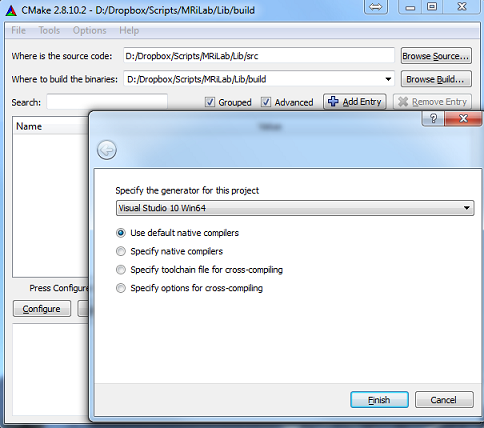
\includegraphics[width=0.7\textwidth]{Pictures/cmake-gui.eps}
			\caption{The cmake-gui for locating source folder and build folder}
			\label{fig:cmake-gui}
		\end{figure}
	\item Step 2 : Configure and generate Visual Studio projects in cmake-gui (Figure \ref{fig:cmake-gui2})
		\begin{figure}[htbp]
			\centering
				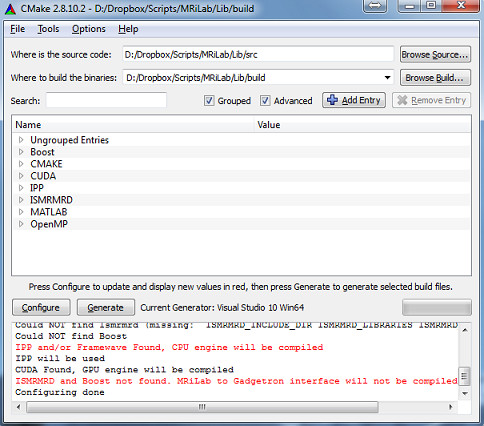
\includegraphics[width=0.7\textwidth]{Pictures/cmake-gui2.eps}
			\caption{The cmake-gui for configuring and building Visual Studio projects}
			\label{fig:cmake-gui2}
		\end{figure}
	\item Step 3 : Build the INSTALL project, compiled MEX binaries will be copied to MRiLab/Lib/bin folder by default (Figure \ref{fig:visualstudio})
		\begin{figure}[htbp]
			\centering
				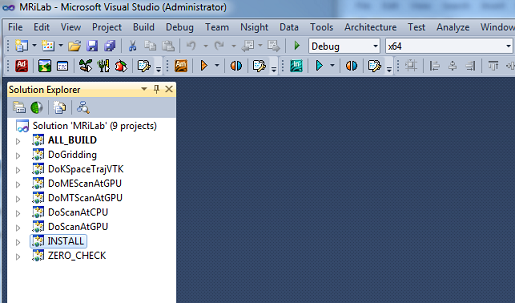
\includegraphics[width=0.7\textwidth]{Pictures/visualstudio.eps}
			\caption{Build INSTALL project using Visual Studio}
			\label{fig:visualstudio}
		\end{figure}
	
\end{itemize}

\end{enumerate}

If installation problems do occur to you, feel free to let me know and I may help you out. For your information, I provide here my development environment (Table \ref {tab:FangSComputerEnvironment}) for the current MRiLab version.

\begin{table}[htbp]
	\centering
		\begin{tabular}{l l l}
	    \hline\hline
			Environment & Desktop & Laptop \\
			\hline
			Machine & Dell Precision T3500 & Lenovo Thinkpad R61 \\
			CPU & Intel Xeon W3530 & Intel Core2 Duo T8100 \\
			GPU & NVIDIA Quadro 4000 & Null \\
			OS  & Windows 7 64-bit & Linux Fedora 16 64-bit \\
			Matlab & Matlab R2013a 64-bit & Matlab R2012b 64-bit \\
			C Compiler & Visual Studio 10 Win64 & GCC 4.6.3 \\
			VTK & VTK 5.10 & VTK 5.10 \\
			CUDA & CUDA 5.0 & Null \\
			IPP & Intel IPP 7.0 & Intel IPP 7.0 \\
			Framewave & AMD Framewave 1.3 & AMD Framewave 1.3 \\
			\hline
		\end{tabular}
	\caption{Fang's Computer Environment}
	\label{tab:FangSComputerEnvironment}
\end{table}


\chapter{Platform Overview}
\section{MRiLab Simulation Platform}
The MRiLab simulation platform consists of 

\begin{enumerate}
\item A Main Simulation Control Console \\
The main simulation control console (Figure \ref{fig:MainSimulationControlConsole}) behaves analogous to a MR scanner console for graphically adjusting imaging setup and conducting simulation control. Simulation feedback are instantly updated on corresponding information panels during the simulation process.

\begin{figure}[htbp]
	\centering
		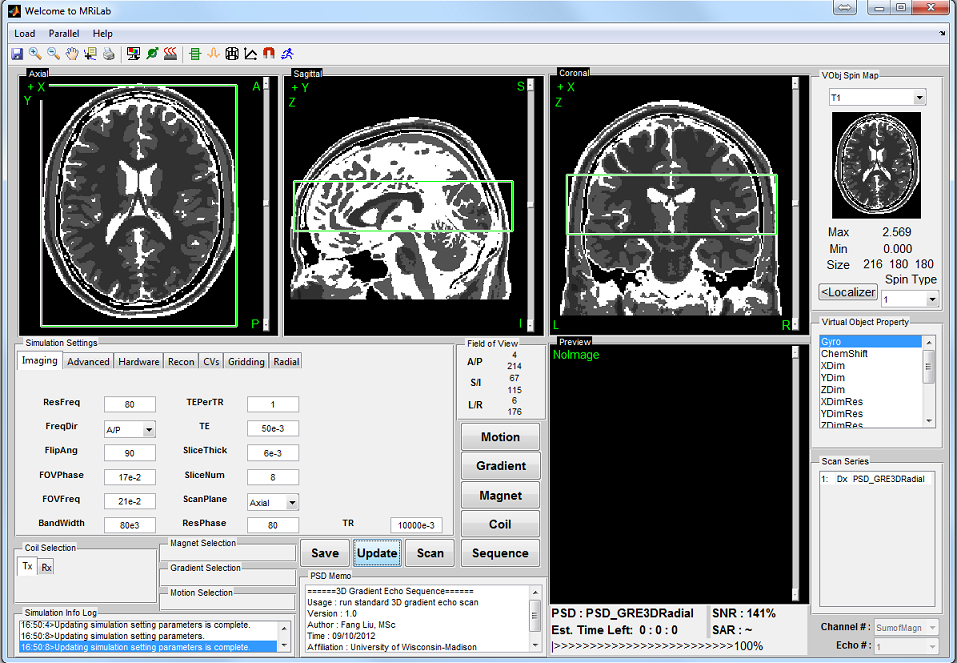
\includegraphics[width=1\textwidth]{Pictures/MainSimulationControlConsole.eps}
	\caption{The MRiLab Main Simulation Control Console. This control console functions like a MR scanner console for graphically adjusting imaging setup and conducting simulation control.}
	\label{fig:MainSimulationControlConsole}
\end{figure}


\item Design Toolboxes \\
The Design toolboxes (Figure \ref{fig:FunctionToolboxes}) provide independent interfaces for designing RF pulse (e.g. SLR, non-adiabatic and adiabatic pulse etc.), for constructing arbitrary pulse sequence (e.g. SPGR, SSFP and FSE etc.), for configuring coil profile and main static magnet field (i.e. B1 and B0 field) and for designing imaging object moving track. Dedicated image display and analysis tools (SpinWatcher, MatrixUser and arrayShow) are also developed and tailored to work with MRiLab simulated high dimensional MR images.


\begin{figure}[htbp]
	\centering
		
\includegraphics{Pictures/FunctionToolboxes.eps}
	\caption{The Shortcut for Function Toolbox on Simulation Control Console. Each icon is associated with an individual toolbox with specific functions.}
	\label{fig:FunctionToolboxes}
\end{figure}


\item Discrete Bloch-equation Solving Kernels \\
The Bloch-equation solving kernels manipulate tissue spin evolution at small discrete time interval in order to accurately simulate spin behavior given a desired spin model and MR sequences. These kernels are accelerated using Matlab MEX functions that are optimized for running GPU and multi-threading CPU parallel computing techniques. Moreover, these kernels are also capable of preprocessing acquired MR signal and K-Space locations prior to desirable image reconstruction. Further image reconstruction with stored K-Space data is accomplished in corresponding reconstruction module.

\item Macro Library \\
MRiLab uses a concept of macros for simplifying experiment design. A macro in MRiLab is defined as a programming-free module that can be added, removed and modified in the process of constructing MR sequence, coil profile, magnet field and object moving track, etc. For instance, a Sinc RF pulse (rfSinc) is considered as a RF macro that can be used for constructing a gradient echo sequence, and the attributes of this macro include pulse starting time (tStart), pulse ending time (tEnd) and the time bandwidth product (TBP) etc. MRiLab provides a macro library (Figure \ref{fig:RFMacroLibrary}) covering a wide range of macros. Using these predefined macros, you should be able to accomplish most of experimental design work. However, if special macros are needed, MRiLab also provides interfaces to work with user-defined macros. More detailed description for macros is provided in Chapter \ref{chap:MRiLabToolboxes}.

\begin{figure}[htbp]
	\centering
		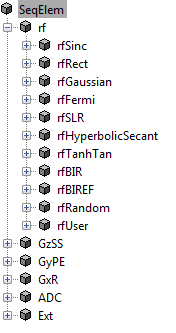
\includegraphics[width=0.3\textwidth]{Pictures/RFMacroLibrary.eps}
	\caption{The Macro Library Tree Structure in MRiLab. Individual tree nodes under SeqElem root are functional macros that can be used for designing MR sequences. Notice that only RF nodes are unfolded here for display purpose.}
	\label{fig:RFMacroLibrary}
\end{figure}

\end{enumerate}
    
MRiLab applies XML files for storing simulation information, which simplifies simulation experiment modification across different studies. MRiLab also supports external plugins programmed using either Matlab or C language for creating extendable simulation system. 

\section{Simulation Workflow}

\begin{figure}[htbp]
	\centering
		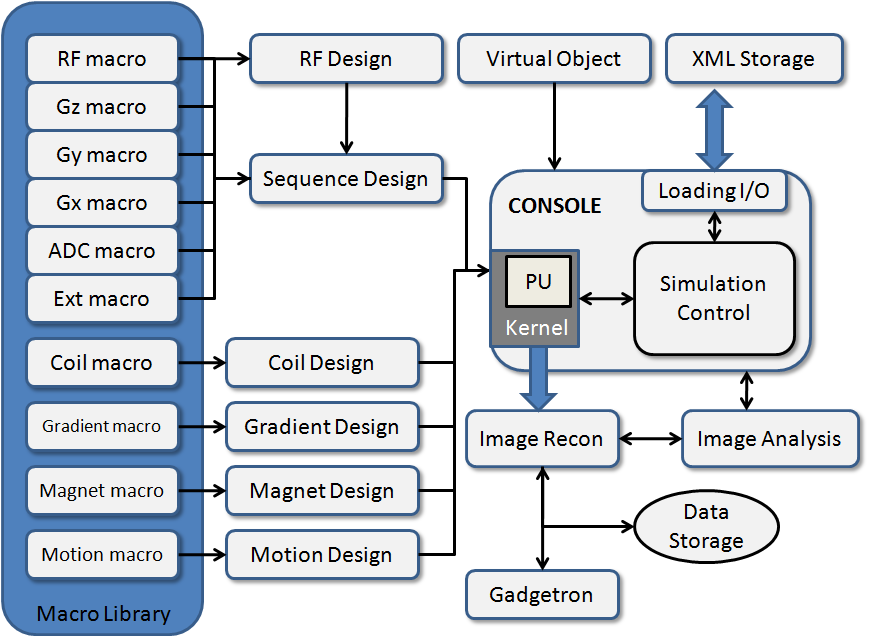
\includegraphics[width=1\textwidth]{Pictures/MRiLabWorkflow.eps}
	\caption{MRiLab Workflow Diagram}
	\label{fig:MRiLabWorkflow}
\end{figure}

The workflow diagram of MRiLab simulation is shown in Figure \ref{fig:MRiLabWorkflow}. One typical simulation requires input of :

\begin{itemize}
	\item Virtual object (VObj) with specific tissue properties including Rho (spin density), T1 and T2 etc.
	\item MR sequence that provides tissue contrast in reconstructed images 
	\item B1 field for RF transmitting and receiving
	\item Gradient field for spatial encoding
	\item Magnet field for describing main static field inhomogeneity (dB0)
	\item Motion pattern for describing imaging object movement during real time simulation
\end{itemize}

All the input information gets configured at the MRiLab main control console where the user can customize any aspect of a simulation experiment. The main console preprocesses the input information then translates them into kernel signal, based on which the discrete solving kernel executes each voxel of imaging objects with either GPU or multi-threading CPU acceleration. The acquired MR signal and K-Space data from the kernel then passes to image reconstruction module where either default recon code or external recon tool (e.g. Gadgetron) is applied. The reconstructed image can be analyzed using MRiLab image display tools including :

\begin{itemize}
	\item MatrixUser : An image display and analysis tool for manipulating multidimensional matrix
	\item SpinWatcher : An analysis tool for analyzing spin evolution behavior within a single voxel
	\item SARWatcher : An analysis tool for analyzing local spatial SAR distribution
	\item arrayShow : A Matlab image viewer for the evaluation of multidimensional complex images
\end{itemize}

\section{Gradient Echo: Start A Simple Scan}

Up to this point, you may wonder how I can start to use MRiLab for imaging simulation. Below is a simple 3D Gradient Echo (GRE) simulation example for you to gain some feelings of using MRiLab.

\begin{itemize}
\item Open MRiLab by running `MRiLab.m' under the root folder. MRiLab will try to detect current available CPU and GPU devices, and initialize the simulation environment. After initialization (typically in couple seconds), MRiLab Main Simulation Control Console will open. Empty Axial, Sagittal, Coronal and Preview views show up. Notice that on the console, several push buttons are disabled at this point, it means more inputs are needed for activating them.
\item To simulate images, the virtual object a.k.a. digital phantom is needed. Go to `Load', `Load Phantom Example', choose one of the predefined digital phantoms for the experiment. A few digital phantoms that are suitable for different experiment purposes are already provided. Here, let's choose `Brain (Standard Resolution 108x90x90)'. After loading this phantom, you will notice the preview image showing up at the top right corner under `VObj Spin Map' and the property information of this phantom are also shown in `Virtual Object Property. Let's choose T2 map from the pop-up menu, and click `Localizer' button to show more image details. Now Axial, Sagittal and Coronal axes are filled with this 3D digital phantom. \textbf{Click `Update' button to accept this phantom loading.} Notice that after updating, all push buttons become enabled.
\item Since we want to simulate 3D GRE experiment, we need to load 3D GRE sequence first. Click the `Sequence' button located at the center portion of the console. A SeqList will open where you can choose and load MR sequences. Let's click `Dimension' pop-up menu and choose `3D'. The Category list shows a full list of current available sequence type. Click `GradientEcho', then click `PSD\_GRE3D' from the Sequence list. Click `Accept' button to accept and load a 3D GRE sequence. Notice that the `Simulation Settings' tabs on the console update and change to the setting for the current GRE sequence. \textbf{Click `Update' button to accept this sequence loading.}
\item Under the `Imaging' tab, there are several parameters for imaging control, for instance, Field-of-View in the frequency encoding direction (FOVFreq). We can simply accept the default setting at this moment, however, if you do make any changes, \textbf{you need to click `Update' button to update those changes before proceeding to Scan.}
\item The final step is to click `Scan' button and wait for the simulation to be performed. Depending on imaging setting and computing hardware, typically the simulation will finish in a short period of time, the reconstructed image will be shown in the `Preview' view.
\end{itemize}

The final looks of this 3D GRE experiment should be somewhat similar to this (Figure \ref{fig:3DGRESampleScan}).


\begin{figure}[htbp]
	\centering
		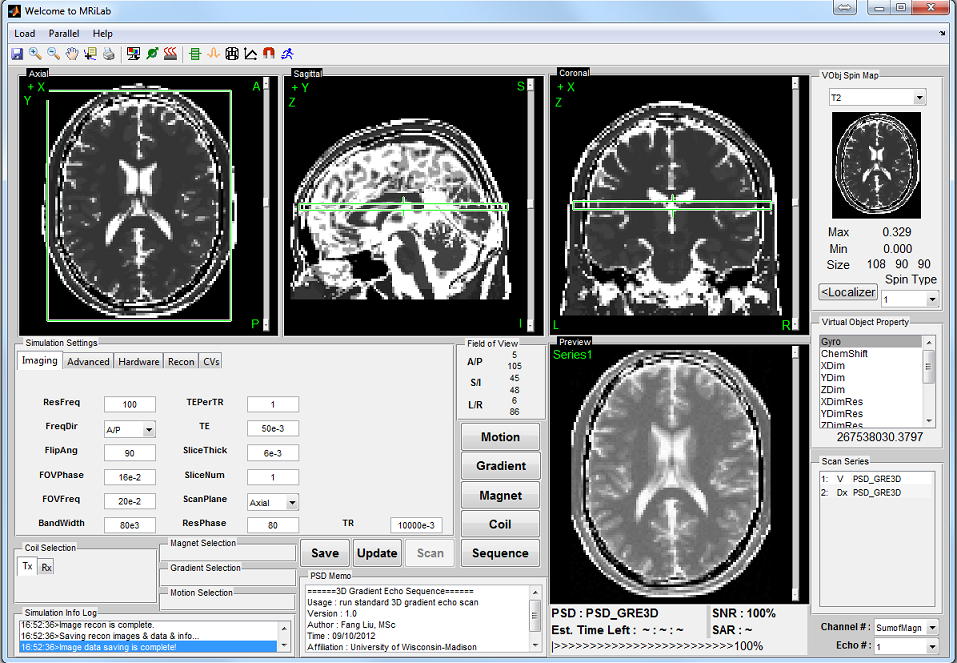
\includegraphics[width=1\textwidth]{Pictures/3DGRESampleScan.eps}
	\caption{The Final Simulation Result for A 3D GRE Experiment}
	\label{fig:3DGRESampleScan}
\end{figure}

If you managed to simulate this gradient echo image, congratulations! You have successfully performed your first MRiLab experiment. So you should be prepared for deeper understanding of MRiLab simulation platform by following the rest of this user guide.


\chapter{Simulation Settings}

\section{Loading Virtual Object}

Prior to perform any type of simulation in MRiLab, a virtual object has to be loaded first. To load virtual object, go to menu `Load' and `Load Phantom' to load a user customized phantom or `Load Phantom Example' to load MRiLab default phantoms. MRiLab provides a few digital phantoms with MR properties mimicking several human tissue types (e.g. Brain, Cartilage, Fat, etc.). After a virtual object being successfully loaded, the geometry of this phantom will show as a preview thumbnail at the top right corner of the console (Figure \ref{fig:VirtualObjectChecking}). The user can inspect phantom property maps of T1, T2 and Rho etc. using the pop-up menu above the thumbnail. If multiple spin species exist in the phantom, the user can also inspect different spin type by using `Spin Type' pop-up menu below the thumbnail. Moreover, a complete list of phantom property of the virtual object is provided at the `Virtual Object Property' list, the user can check any of them by clicking the corresponding item. A complete property list of one virtual object typically include:

\begin{itemize}
	\item Gyro (rad/s/T) : The gyromagnetic ratio of the spin
	\item ChemShift (Hz/T) : The chemical shift of the spin
	\item XDim : The number of voxels in X direction
	\item YDim : The number of voxels in Y direction
	\item ZDim : The number of voxels in Z direction
	\item XDimRes (m) : The voxel size in X direction
	\item YDimRes (m) : The voxel size in Y direction
	\item ZDimRes (m) : The voxel size in Z direction
	\item Type : A description of the type of the spin
	\item TypeNum : The number of spin species
	\item Rho : A matrix with the size of $ YDim \times XDim \times ZDim \times TypeNum $ for describing spin density
	\item T1 (s) : A matrix with the size of $ YDim \times XDim \times ZDim \times TypeNum $ for describing T1 relaxation time
	\item T2 (s) : A matrix with the size of $ YDim \times XDim \times ZDim \times TypeNum $ for describing T2 relaxation time
	\item T2Star (s) : A matrix with the size of $ YDim \times XDim \times ZDim \times TypeNum $ for describing T2* relaxation time
\end{itemize}

\begin{figure}[htbp]
	\centering
		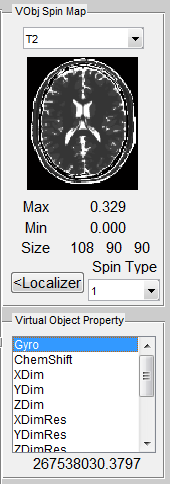
\includegraphics[width=0.3\textwidth]{Pictures/VirtualObjectChecking.eps}
	\caption{A Virtual Object Preview}
	\label{fig:VirtualObjectChecking}
\end{figure}

To inspect more details of the digital phantom, press the `Localizer' button to populate the thumbnail to the main image display panel. MRiLab provides three image axes to display axial, sagittal and coronal view section of the three dimensional virtual object, respectively. A scroll bar beside each axes allows to change image slice along the corresponding direction, which serves as an anatomical reference for prescribing simulation parameters. For instance, the location of a green box in each axes indicating current field of view can be adjusted via free hand dragging, and the field of view location is instantly updated at `Field of View' panel upon dragging.

\section{Loading Sequence}
One of the key features of MRiLab is allowing simulating a wide range of MR sequences and facilitating investigation and optimization of desirable MR contrast among different tissues. MRiLab provides a sequence loading interface allowing users to choose predefined sequences from default MRiLab sequence library, or choose other user customized sequences. MRiLab parses a selected MR sequence and translates the sequence waveform into specific signal which triggers simulation kernel execution. The sequence loading interface provides functions to load MR sequence. A MR sequence design toolbox is separate from loading interface and will be explained in detail in Chapter \ref{chap:MRiLabToolboxes}.

\subsection{Loading Predefined Sequence}

\begin{figure}[htbp]
	\centering
		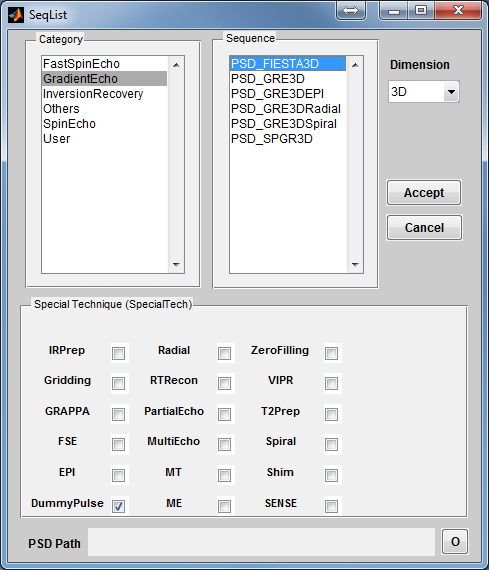
\includegraphics[width=0.8\textwidth]{Pictures/SequenceLoading.eps}
	\caption{The Sequence Loading Interface. A sequence named PSD\_FIESTA3D from 3D GradientEcho Category is chosen, and DummyPulse special technique is checked by default.}
	\label{fig:SequenceLoading}
\end{figure}

To open a sequence loading interface (Figure \ref{fig:SequenceLoading}), click the `Sequence' button located at the center portion of the main control console. Once the interface is open, the `Dimension' specifies the sequence spatial encoding scheme (2D or 3D). The `Category' provides a list of sequence classes including Gradient Echo, Spin Echo, Inversion Recovery, Fast Spin Echo, Others and User. Upon clicking one sequence category, a few sequences belonging to the selected category become available in the sequence list on the right. Click a sequence, then press `Accept' to load the selected sequence. pressing `Cancel' button will close the interface without loading any sequence. \\

Notice there is a `Special Technique (SpecialTech)' panel below the sequence list. If a sequence using any of special techniques is selected, the corresponding checkboxes beside the special techniques will be chosen. For example, by default PSD\_FIESTA3D uses the special techniques called DummyPulse, therefore, by clicking PSD\_FIESTA3D, the DummyPulse will be chosen accordingly. However, you can uncheck the checkbox for avoiding the DummyPulse module, but this may cause incomplete simulation for PSD\_FIESTA3D. It is recommended to keep default selection of special techniques therefore a complete sequence control is preserved for those default sequences. On the other hand, for the sequences that have no special techniques, you can also add special technique module by checking corresponding checkbox. This will load parameter tabs of special techniques on the simulation control console for configuration purpose. The special technique strategy enables the ability for reusing `capsulized' module for different sequences. \\

MRiLab provides a few default sequences under the folder /PSD, notice the /PSD folder uses the same hierarchic structure scheme as that of the loading interface. Typically a new sequence can be located anywhere in the computer, however it is recommended to save the sequence under those predefined categories under /PSD therefore they are visible to the loading interface. However, if a customized sequence is not directly visible to the loading interface, it can also be loaded using the PSD loading button marked as `o' at the bottom of the loading interface. If the PSD loading button is used, loading interface will ignore regular sequence selection.

\subsection{Predefined Sequences}
MRiLab provides a few predefined MR sequences including

\begin{enumerate}
	\item Fast Spin Echo 
	
	\begin{itemize}
	\item PSD\_FSE3D \\
	Three dimensional multishot Fast Spin Echo (FSE) sequence with interleaved K-Space sampling in Kx-Ky and conventional phase-encoding along Kz. 
\end{itemize}

\item Gradient Echo

\begin{itemize}
	\item PSD\_FIESTA3D \\
	Three dimensional balanced Steady State Free Precession (bSSFP) sequence.
	\item PSD\_SPGR3D \\
	Three dimensional Spoiled Gradient Echo (SPGR) sequence.
	\item PSD\_GRE3D \\
	Three dimensional gradient echo sequence with Cartesian readout.
	\item PSD\_GRE3DEPI \\
	Three dimensional gradient echo sequence with multishot Echo Planar Imaging (EPI) readout using interleaved K-Space sampling in Kx-Ky and conventional phase-encoding along Kz. 
	\item PSD\_GRE3DRadial \\
	Three dimensional gradient echo sequence with radial readout in Kx-Ky and conventional phase-encoding along Kz, usually referred to as stack-of-stars sequence.
	\item PSD\_GRE3DSpiral \\
	Three dimensional gradient echo sequence with multishot spiral readout in Kx-Ky and conventional phase-encoding along Kz, referred to as stack-of-spiral sequence. 
\end{itemize}

\item Inversion Recovery
\begin{itemize}
	\item PSD\_IR3D \\
	Three dimensional Inversion Recovery (IR) sequence with Cartesian readout.
\end{itemize}

\item SpinEcho
\begin{itemize}
	\item PSD\_SE3D \\
	Three dimensional Spin Echo (SE) sequence with Cartesian readout.
\end{itemize}

\item User
\begin{itemize}
	\item PSD\_SPGR3DMT \\
	Three dimensional SPGR sequence with Magnetization Transfer (MT) saturation. Note that MT phantom is needed for running this sequence.
	\item PSD\_SPGR3DME \\
	Three dimensional SPGR sequence for Multiple spin pool exchange (ME) model. Note that ME phantom is needed for running this sequence.
\end{itemize}

\item Others
\begin{itemize}
	\item PSD\_AFI \\
	Three dimensional SPGR sequence for performing flip angle mapping using Actual Flip Angle Imaging (AFI) technique \cite{Yarnykh2007}.
\end{itemize}

\end{enumerate}


\section{Loading Coil}
To simulate multi-transmitting and receiving coil, MRiLab provides a coil loading interface allowing to choose different coil configurations for Tx (i.e. Transmitting) and/or Rx (i.e. Receiving). MRiLab translates the coil configuration and computes a B1+/B1- field accordingly. For multi-transmitting coil, each coil element could be treated separately and receives individual RF signal source. This allows to investigate B1 shimming and multiple RF excitation etc. For multi-receiving coil, each coil element also connects to an individual signal channel and produces signal according to its specific coil sensitivity. This allows to investigate coil encoding methods such as parallel imaging. The coil loading interface provides functions to load coil configuration. A coil design toolbox is separate from loading interface and will be explained in detail in Chapter \ref{chap:MRiLabToolboxes}.

\subsection{Loading Predefined Coil}

\begin{figure}[htbp]
	\centering
		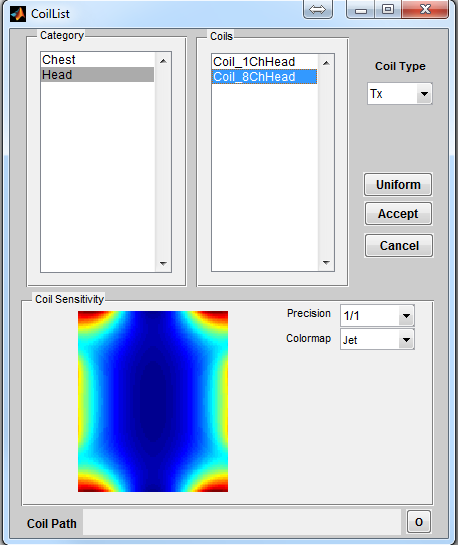
\includegraphics[width=0.8\textwidth]{Pictures/CoilLoading.eps}
	\caption{The Coil Loading Interface. An eight channel coil configuration named Coil\_8ChHead from Head Category is chosen, preview image shows the total coil sensitivity with the same spatial resolution as that of the chosen digital phantom.}
	\label{fig:CoilLoading}
\end{figure}

To open a coil loading interface (Figure \ref{fig:CoilLoading}), click the `Coil' button located at the center portion of the console. The `Category' list specifies different coil configuration category based on anatomical structure. The `Coils' list beside the `Category' list provides coil configuration belonging to the selected category. Upon clicking a coil configuration, the interface will calculate the coil sensitivity map and display it in the preview axes. The user can specify displaying spatial resolution using the `Precision' with a highest spatial resolution defined as the same resolution of digital phantom. Moreover, the user can specify color map from `Jet',`Gray' or `Hot'. Pressing `Accept' will load the selected coil configuration. However, pressing `Cancel' button will close the interface without loading any coil configuration. If an uniform unit coil sensitivity is desired, press `Uniform' button to load that. By default, MRiLab uses an uniform unit coil sensitivity for both RF transmitting and receiving. To indicate an usage of the selected coil configuration, the user has to specify `Coil Type' as either Tx for transmitting or Rx for receiving. \\ 

MRiLab provides a few default coil configuration under the folder /Coil, notice the /Coil folder uses the same hierarchic structure scheme as that of the loading interface. Typically a new coil configuration can be located anywhere in the computer, however it is recommended to save the coil configuration folder under those predefined categories under /Coil therefore they are visible to the loading interface. However, if a customized coil configuration is not directly visible to the loading interface, it can also be loaded using the Coil loading button marked as `o' at the bottom of the loading interface. If the Coil loading button is used, loading interface will ignore regular coil selection.

\subsection{Predefined Coil}

MRiLab provides a few predefined coil configuration including

\begin{enumerate}
		\item Head
		\begin{itemize}
			\item Coil\_1ChHead \\
			A coil configuration consists of one single Biot-Savart circle, primarily used for testing purpose.
			\item Coil\_8ChHead \\
			A coil configuration consists of 8 Biot-Savart circles, which produces relative flat B1 field in X-Y plane along X direction.
		\end{itemize}
		
		\item Chest
		\begin{itemize}
			\item Coil\_9ChSurfChest \\
			A coil configuration consists of 9 Biot-Savart circles, which produces relative flat B1 field in X-Y plane along Y direction at the surface region.
		\end{itemize}
\end{enumerate}


\section{Loading Magnet}

MR simulation studies may need to use non-uniform magnetic field. Those studies include the ones for investigating susceptibility artifact, and developing less field inhomogeneity sensitive sequences. MRiLab provides the magnet loading interface allowing to load customized B0 field inhomogeneity map (i.e. dB0 map, a map for indicating main field variation). The magnet loading interface provides functions to load dB0 map. A magnet design toolbox is separate from loading interface and will be explained in detail in Chapter \ref{chap:MRiLabToolboxes}.

\subsection{Loading Predefined Magnet}

\begin{figure}[htbp]
	\centering
		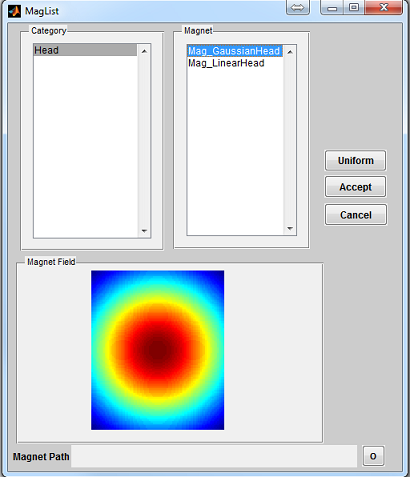
\includegraphics[width=0.8\textwidth]{Pictures/MagnetLoading.eps}
	\caption{The Magnet Loading Interface. A magnet named Mag\_GaussianHead from Head Category is chosen, preview image shows the dB0 map in the X-Y plane with the same spatial resolution as that of the chosen digital phantom.}
	\label{fig:MagnetLoading}
\end{figure}

To open a magnet loading interface (Figure \ref{fig:MagnetLoading}), click the `Magnet' button located at the center portion of the console. The `Category' list specifies different magnet category based on anatomical structure. The `Magnet' list beside the `Category' list provides magnet belonging to the selected category. Upon clicking a magnet file, the interface will compute a dB0 map and display it in the preview axes. Pressing `Accept' will load the chosen magnet profile. However, pressing `Cancel' button will close the interface without loading any profile. If an uniform B0 field (i.e. zero dB0) is desired, press `Uniform' button to load that. By default, MRiLab uses an uniform B0 field for simulation. That is to say there is no field inhomogeneity across the entire virtual object. \\

MRiLab provides a few default magnet profile under the folder /Mag, notice the /Mag folder uses the same hierarchic structure scheme as that of the loading interface. Typically a new magnet profile can be located anywhere in the computer, however it is recommended to save the magnet profile folder under those predefined categories under /Mag therefore they are visible to the loading interface. However, if a customized magnet is not directly visible to the loading interface, it can also be loaded using the Magnet loading button marked as `o' at the bottom of the loading interface. If the loading button is used, loading interface will ignore regular magnet selection.

\subsection{Predefined Magnet}

MRiLab provides two predefined magnet configuration including

\begin{enumerate}
		\item Head
		\begin{itemize}
			\item Mag\_GaussianHead \\
			A magnet profile produces a Gaussian dB0 field in three dimensional space.
			\item Mag\_LinearHead \\
			A magnet profile produces a linear dB0 field in three dimensional space.
		\end{itemize}

\end{enumerate}

\section{Loading Gradient}
Regular MR spatial encoding is performed in a linear (flat) fashion. However encoding in a nonlinear (curved) fashion may serve particular purposes in some MR studies. MRiLab provides a gradient loading interface to load customized 3D nonlinear gradient field. This function can help investigate arbitrary curved gradient field for imaging simulation. Benefit from MRiLab's powerful functionality of MR sequence design, nonlinear gradient encoding techniques such as PatLoc can be simulated with minimal efforts in MRiLab. The gradient loading interface provides functions to load nonlinear gradient. A gradient design toolbox is separate from the loading interface and will be explained in detail in Chapter \ref{chap:MRiLabToolboxes}.

\subsection{Loading Predefined Gradient}

\begin{figure}[htbp]
	\centering
		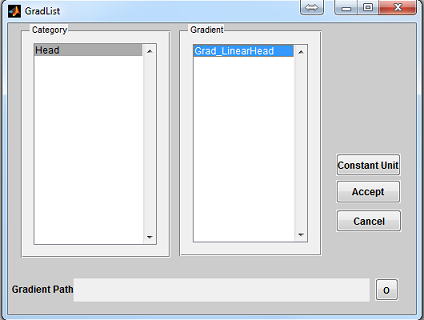
\includegraphics[width=0.8\textwidth]{Pictures/GradientLoading.eps}
	\caption{The Gradient Loading Interface. A gradient profile named Grad\_LinearHead from Head Category is chosen.}
	\label{fig:GradientLoading}
\end{figure}

To open a gradient loading interface (Figure \ref{fig:GradientLoading}), click the `Gradient' button located at the center portion of the console. The `Category' list specifies different gradient category based on the anatomical structure. The `Gradient' list beside the `Category' list provides gradient profile belonging to the selected category. Upon clicking a gradient configuration, pressing `Accept' will load the selected gradient profile. However, pressing `Cancel' button will close the interface without loading any gradient profile. If a constant unit gradient is desired, press `Constant Unit' button to load that. By default, MRiLab uses a constant unit gradient profile in the X, Y and Z direction for a typical gradient simulation. This will maintain a conventional linear spatial encoding in all three spatial dimensions. \\

MRiLab provides gradient profiles under the folder /Grad, notice the /Grad folder uses the same hierarchic structure scheme as that of the loading interface. Typically a new gradient profile can be located anywhere in the computer, however it is recommended to save the gradient profile under those predefined categories under /Grad therefore they are visible to the loading interface. However, if a customized gradient is not directly visible to the loading interface, it can also be loaded using the Gradient loading button marked as `o' at the bottom of the loading interface. If the Gradient loading button is used, loading interface will ignore regular gradient selection.

\subsection{Predefined Gradient}

MRiLab provides one predefined example of gradient profile

\begin{enumerate}
		\item Head
		\begin{itemize}
			\item Grad\_LinearHead \\
			A gradient profile produces constant gradient field with varying gradient value in three dimensions, which can cause image contraction, expansion or shearing etc.
		\end{itemize}
\end{enumerate}


\section{Loading Motion}
MRiLab provides a motion simulation mechanism which implements simulating imaging object movement in three dimensional space. MRiLab's Motion simulation introduces an approach for simulating four dimensional imaging (3D space + time) techniques such as k-t blast and enables developing real time image reconstruction algorithms. It also helps investigate motion insensitive sequence and test motion artifact in various types of sequences and conditions. The motion loading interface provides functions to load motion trajectory. A motion design toolbox is separate from the loading interface and will be used for designing motion pattern in three dimensional space.


\subsection{Loading Predefined Motion}

\begin{figure}[htbp]
	\centering
		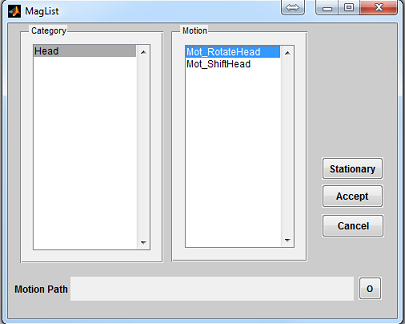
\includegraphics[width=0.8\textwidth]{Pictures/MotionLoading.eps}
	\caption{The Motion Loading Interface. A motion profile named Mot\_RotateHead from Head Category is chosen. This motion profile create object rotation in three dimensions along any user defined axis.}
	\label{fig:MotionLoading}
\end{figure}

To open a motion loading interface (Figure \ref{fig:MotionLoading}), click the `Motion' button located at the center portion of the console. The `Category' list specifies different motion category based on the anatomical structure. The `Motion' list beside the `Category' list provides motion profile belonging to the selected category. Upon clicking a motion pattern, pressing `Accept' will load the chosen motion profile. However, pressing `Cancel' button will close the interface without loading any motion profile. If motion isn't desirable, press `Stationary' button. By default, no motion is used in MRiLab simulation. \\

MRiLab provides motion profiles under the folder /Mot, notice the /Mot folder uses the same hierarchic structure scheme as that of the loading interface. Typically a new motion profile can be located anywhere in the computer, however it is recommended to save the motion profile under those predefined categories under /Mot therefore they are visible to the loading interface. However, if a customized motion is not directly visible to the loading interface, it can also be loaded using the Motion loading button marked as `o' at the bottom of the loading interface. If the Motion loading button is used, loading interface will ignore regular motion selection.

\subsection{Predefined Motion}

MRiLab provides two predefined examples of motion profile

\begin{enumerate}
		\item Head
		\begin{itemize}
			\item Mot\_RotateHead \\
			A motion profile produces object rotation in three dimensional space along any user defined axis.
			\item Mot\_ShiftHead \\
			A motion profile produces object translation in any user defined direction.
		\end{itemize}
\end{enumerate}

\section{Prescribing Scan Parameters}

Those loading interfaces offer a mechanism to interpret and convert configuration file into MRiLab parameters. With a successful loading, the `Coil Selection', `Magnet Selection',`Gradient Selection' and `Motion Selection' fields indicate the current selected configuration. The user can change the configuration by reloading a new configuration file with above mentioned steps. If any of these fields are empty, a default setting will be used. Similar to a real scanner system, MRiLab categorizes scanning parameters into different groups and present them under different tabs in the `Simulation Settings' panel (Figure \ref{fig:SimulationSettings}). There are five tabs which are included in all MR sequences, including Imaging, Advanced, Hardware, Recon and CVs. Additional tabs for special techniques will also become valid if those techniques are loaded from sequence selection. Below are detailed explanation for each of those parameters.

\begin{figure}[htbp]
	\centering
		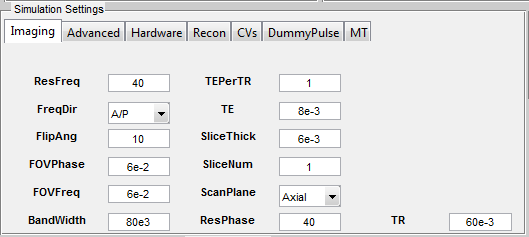
\includegraphics[width=1\textwidth]{Pictures/SimulationSettings.eps}
	\caption{The Simulation Settings Panel. The panel contains Imaging, Advanced, Hardware, Recon and CVs tabs, two additional special technique DummyPulse and MT are also added for this sequence.}
	\label{fig:SimulationSettings}
\end{figure}

\section{Parameter List}

Below are a full list of supported simulation parameters in current MRiLab version. Notice that unless otherwise specified, MRiLab uses International System of Units (i.e. SI units) for all the parameters.

\subsection{Imaging}
The `Imaging' tab contains parameters relevant to image resolution, field of view and timing setting etc.
	\begin{itemize}
		\item BandWidth (Hz) : Full receiver bandwidth
		\item FOVFreq (m) : Field of view in the frequency encoding direction
		\item FOVPhase (m) : Field of view in the first phase encoding direction
	  \item FlipAng (Degree) : Flip angle of excitation pulse
		\item FreqDir : Frequency encoding direction
		\item ResFreq : Number of voxels in frequency encoding direction
		\item ResPhase : Number of voxels in the first phase encoding direction
		\item ScanPlane : The scanning plane
		\item SliceNum : The number of encoding slice
		\item SliceThick (m) : The thickness of one slice
		\item TE (s) : The time of echo
		\item TEPerTR : The number of echoes in multiple echo mode, using a number above one requires `MultiEcho' tab to be loaded
		\item TR (s) : The time of repetition
	\end{itemize}

\subsection{Advanced}
The `Advanced' tab contains other imaging parameters.
	\begin{itemize}
		\item MasterTxCoil : The master transmitting coil in multi RF transmitting mode
		\item MultiTransmit : The flag for turning on and off multi RF transmitting mode, default mode is `off' for single RF transmitting
		\item NEX : The number of excitation
	  \item NoFreqAlias : The flag for avoiding aliasing in frequency encoding direction, default `on' truncates object outside field of view in frequency encoding direction
		\item NoPhaseAlias : The flag for avoiding aliasing in the first phase encoding direction, default `on' truncates object outside field of view in the first phase encoding direction
		\item NoSliceAlias : The flag for avoiding aliasing in the second phase encoding (i.e. slice encoding) direction, default `on' truncates object outside field of view in slice encoding direction
		\item Shim : The flag for choosing shimming mode
		\item TEAnchor : The flag for choosing TE time offset regarding the RF pulse width
	\end{itemize}

\subsection{Hardware}
The `Hardware' tab contains parameters relevant to system hardware setup.
	\begin{itemize}
		\item B0 (T) : Main static magnetic field strength
		\item B1Level (T) : A reference B1 field strength which produces nominal prescribed flip angle
		\item MaxGrad (T/m) : Maximum allowable gradient strength
	  \item MaxSlewRate (T/m/s) : Maximum allowable gradient slew rate
		\item MinUpdRate (s) : Minimum update time on generating sequence waveform
		\item Model : A real scanner system with the possibly most similar hardware setting
		\item NoiseLevel :  The level of adjustable noise, the higher the number, the more noise
		\item SpinPerVoxel : The number of spins in each voxel, default one spin per voxel will treat T2* equal to T2, use a number above one for simulating T2* effect (time consuming)
	\end{itemize}

\subsection{Recon}
The `Recon' tab contains parameters relevant to image reconstruction.
	\begin{itemize}
		\item AutoRecon : The flag for turning on and off automatic image reconstruction after MR signal acquisition
		\item ExternalEng : The name of a user defined script for image reconstruction
		\item OutputType : The type of output data including both simulated image and signal, options include `MAT' and `ISMRMRD', the latter requires ISMRMRD dependency packages to be installed
	  \item ReconEng : The image reconstruction engine, choosing `Default' uses MRiLab default reconstruction code, choosing `External' uses external engine which requires ExternalEng to be provided
		\item ReconType :  The type of image reconstruction
	\end{itemize}

\subsection{CVs}
The `CVs' tab contains Controllable Variables (CV) which exist in the global scope of sequence design. They are designed for conveniently transferring values among multiple MR sequence modules. The user can use them for customized purpose.
	\begin{itemize}
		\item CV1 : Controllable variable 1
		\item CV2 : Controllable variable 2
		\item CV3 : Controllable variable 3
		\item CV4 : Controllable variable 4
		\item CV5 : Controllable variable 5
		\item CV6 : Controllable variable 6
		\item CV7 : Controllable variable 7
		\item CV8 : Controllable variable 8
		\item CV9 : Controllable variable 9
		\item CV10 : Controllable variable 10
		\item CV11 : Controllable variable 11
		\item CV12 : Controllable variable 12
		\item CV13 : Controllable variable 13
		\item CV14 : Controllable variable 14
	\end{itemize}

\subsection{SpecialTech}

The Special Technique (SpecialTech) contains multiple tabs from which one or more are loaded based on sequence configuration and user choice.

\begin{enumerate}
	\item DummyPulse \\
	The `DummyPulse' tab are designed for adding dummy pulse section before image acquisition section. It can be used for skipping transient steady state signal.
		\begin{itemize}
			\item DP\_Flag : The flag for turning on and off dummy pulse
			\item DP\_FlipAng (Degree) : The flip angle of excitation pulse for dummy pulse
			\item DP\_Num : The number of TRs for dummy pulse
			\item DP\_TR (s) : The time of repetition for dummy pulse
		\end{itemize}
	
  \item	EPI \\
	The `EPI' tab contains parameters for performing multi shot interleaved EPI readout.
		\begin{itemize}
			\item EPI\_ESP (s) : The echo spacing for EPI
			\item EPI\_ETL : The echo train length for EPI
			\item EPI\_EchoShifting : The flag for turning on and off echo shifting
			\item EPI\_ShotNum : The number of EPI shots, multi shot EPI uses interleave mode
		\end{itemize}
		
	\item FSE \\
	The `FSE' tab contains parameters for performing multi shot interleaved FSE readout.
		\begin{itemize}
			\item FSE\_ESP (s) : The echo spacing for FSE
			\item FSE\_ETL : The echo train length for FSE
			\item FSE\_ShotNum : The number of FSE shots, multi shot FSE uses interleave mode
		\end{itemize}
		
  \item GRAPPA (:TODO) \\
	The `GRAPPA' tab contains parameters for performing parallel imaging using GRAPPA.
	
  \item Gridding \\
	The `Gridding' tab contains parameters for controlling gridding process in default Non-Cartesian reconstruction. MRiLab uses Voronoi diagram for K-Space density compensation, and uses Kaiser-Bessel kernel for gridding. Detailed explanation is beyond the scope of this manual, users who are interested are referred to \cite{Jackson1991,VRasche1999,Beatty2005}.
		\begin{itemize}
			\item G\_Deapodization : The flag for turning on and off kernel deapodization (i.e. dividing reconstructed image with the iFFT of the gridding kernel)
			\item G\_KernelSample : The number of kernel sample point, the more sample points, the better kernel approximation
			\item G\_KernelWidth : The full width of kernel in the unit of gridding grid
			\item G\_OverGrid : The over gridding factor
			\item G\_Truncation : The flag for turning on and off image truncation for reconstructed image
		\end{itemize}
	
	\item IRPrep \\
	The `IRPrep' tab contains parameters for inversion recovery sequence.
		\begin{itemize}
			\item TI (s) : The time of inversion recovery
		\end{itemize}
		
	\item MT \\
	The `MT' tab contains parameters for activating MR sequences running Magnetization Transfer model (MT). In order to perform MT experiment, MT phantom is required.
		\begin{itemize}
			\item MT\_Flag : The flag for turning on and off MT simulation
		\end{itemize}
		
	\item ME \\
	The `ME' tab contains parameters for activating MR sequences running Multiple pool spin Exchange model (ME). In order to perform ME experiment, ME phantom is required.
	\begin{itemize}
		\item ME\_Flag : The flag for turning on and off ME simulation
	\end{itemize}
	
	\item RTRecon \\
	The `RTRecon' tab contains parameters for performing real time image reconstruction. Notice that adding RTRecon tab is not guaranteed to perform real time reconstruction, the user also needs to use the extended real time process to trigger real time image reconstruction at the Ext sequence line. See Section \ref{subs:ExtMacroLibrary} for more details.
	\begin{itemize}
		\item RTR\_Flag : The flag for turning on and off real time reconstruction
		\item PlotK\_Flag : The flag for turning on and off real time K-Space plotting
		\item DelayTime : The delay time for refreshing graphics
	\end{itemize}
		
  \item MultiEcho \\
	The `MultiEcho' tab contains parameters for performing multi echo experiment, the number of echoes much match TEPerTR.
		\begin{itemize}
			\item ME\_TEs (s) : An array of multiple echo values
		\end{itemize}
	
	\item PartialEcho (:TODO) \\
	The `PartialEcho' tab contains parameters for performing partial echo in readout.
	
	\item Radial \\
	The `Radial' tab contains parameters for performing 2D radial readout sampling.
		\begin{itemize}
			\item R\_AngPattern : The pattern for sampling the angle in K-Space
			\item R\_AngRange : The range of sampling angle
			\item R\_SampPerSpoke : The number of sampling points in each spoke
			\item R\_SpokeNum : The number of sampling spokes
		\end{itemize}
	
  \item SENSE (:TODO) \\
	The `SENSE' tab contains parameters for performing parallel imaging using SENSE.
	
	\item Shim \\
	The `Shim' tab contains parameters for performing manual B0 shimming.
		\begin{itemize}
			\item Sh\_X : The constant for X term
			\item Sh\_Y : The constant for Y term
			\item Sh\_Z :  The constant for Z term
			\item Sh\_ZX : The constant for ZX term
			\item Sh\_ZY : The constant for ZY term
			\item Sh\_Z2 : The constant for Z\textsuperscript{2} term
			\item Sh\_XYZ : The constant for XYZ term
			\item Sh\_X2\_Y2 : The constant for X\textsuperscript{2}Y\textsuperscript{2} term
		\end{itemize}
	
	\item Spiral \\
	The `Spiral' tab contains parameters for performing multi shot spiral readout. The 2D spiral design uses a method described in \cite{Glover2005}.
		\begin{itemize}
			\item S\_Gradient (T/m) : The desired gradient amplitude
			\item S\_Lamda (1/m/rad) : A constant affecting radial sampling interval in the spiral trajectory
			\item S\_ShotNum : The number of spiral interleaves
			\item S\_SlewRate (T/m/s) : The desired slew rate. Notice that in this approximation, slew rate overshoots the desired value for part of the slew-rate-limited region
			\item S\_SlewRate0 (T/m/s) : The slew rate at the beginning
		\end{itemize}
	
  \item T2Prep (:TODO) \\
	The `T2Prep' tab contains parameters for T2 preparation sequence.
	
	\item VIPR (:TODO) \\
	The `VIPR' tab contains parameters for performing Vastly Undersampled Isotropic Projection Reconstruction (VIPR) sequence.
	
	\item ZeroFilling \\
	The `ZeroFilling' tab contains parameters for performing image interpolation in the K-Space using zero filling.
		\begin{itemize}
			\item ZF\_Kz : The zero filling factor in Kz
			\item ZF\_Ky : The number of point in Ky after zero filling
			\item ZF\_Kx : The number of point in Kx after zero filling
		\end{itemize}
	
\end{enumerate}

\section{Parallel Computing}

The current MRiLab version supports two types of parallel computing mechanisms: GPU based parallel computing using CUDA and multi-threading CPU based parallel computing using OpenMP. As mentioned before, the GPU support requires NVIDIA GPU with CUDA capability (shader model 2.0) along with properly installed GPU driver. The OpenMP is, on the other hand, supported by most of modern multi core CPU. If both GPU and CPU are available in user's system, the user can choose to use any of these two methods. To switch parallel computing methods, go to `Parallel' menu and `Select Processing Unit' and choose available GPU or CPU devices.

\chapter{Simulation}

\section{Running Simulation}

The MRiLab converts simulation parameters from configuration files into temporary configuration structures during loading process, and uses these structures to organize simulation workflow. The user can check the default value of each parameter by moving a mouse cursor on top of selected parameters. The use can adjust loaded simulation parameters to satisfy a simulation design, to make changing parameters effective, the user has to press `Update' button located below `Simulation Settings' panel. The `Update' button not only updates these structures, but also performs a series of pre-scan processes including checking incompatibility error and initializing other necessary simulation variables. \\

On the left of `Update' button, there is a `Save' button which saves updated configuration structure back into corresponding configuration files for later use. One particular case is that `CVs' need to be updated and then saved in order to make changes effective. This is because `CVs' is one part of the sequence file which needs to be interpreted at the sequence waveform generation module. The sequence memo is also provided at the `PSD Memo' panel. It's editable and can be saved using `Save' button. \\

On the right of `Update' button, there is a `Scan' button which activates sequence waveform generation, actual scan process and post-scan process including image reconstruction and data saving. The MRiLab automatically detects any parameter changes and set `Scan' button disabled. To enable `Scan' button, simply press `Update' button. Notice that the update process may take some time if a large number of initialization is needed, so be patient and wait it to finish before proceeding. The `Simulation Info Log' is helpful for checking log information about each simulation step. Once simulation setting gets configured properly, the user can press `Scan' button to start scanning.

\section{Image, SNR and SAR}

\begin{figure}[htbp]
	\centering
		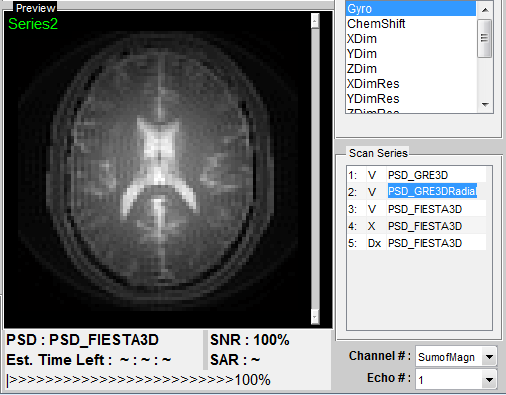
\includegraphics[width=1\textwidth]{Pictures/SimulationImage.eps}
	\caption{A Preview of A Simulated Image. The preview is one slice of simulated image using gradient echo sequence with radial readout and reconstructed without deapodization.}
	\label{fig:SimulationImage}
\end{figure}

Figure \ref{fig:SimulationImage} demonstrates an example of a series of simulation operated with different sequences. Each sequence is labeled with an unique series number, and shows in the list at `Scan Series' panel. This series number is also a reference for the saved image and data in the output database which will be explained in Chapter \ref{chap:MRiLabToolboxes}. There is also a status label on the left of each sequence name. The status labels include:

\begin{itemize}
	\item Dx : parameter setting and sequence loading
	\item ... : scanning
	\item V :  scan complete successfully
	\item X : scan incomplete or fail
\end{itemize}

The example shows a series of successful simulation by using PSD\_GRE3D, PSD\_GRE3DRadial and PSD\_FIESTA3D sequences, but incomplete simulation using PSD\_FIESTA3D at the second time. The preview axes displays an image preview for the series 2 simulated using PSD\_GRE3DRadial sequence. The user can switch previews for successful simulation by clicking scan series item. Moreover, the series name is also editable although in this example the series name is kept the same as the name of the sequence, which is not absolutely necessary. If the multiple channel coil for multiple receiving is performed (Figure \ref{fig:SimulationImage2}), the user can specify display image to any channel with `Channel \#' pop-up menu, or choose `SumofMagn' for summation of image magnitude of all channels or `SumofCplx' for summation of complex image of all channels. If multiple echo is enabled in the sequence, the user can also specify display image to any echo with `Echo \#' pop-up menu. Default value of 1 is used for single echo. The preview image provides a quick overview of the simulated images, a further image analysis can be performed with image display and analysis tools in Chapter \ref{chap:ImageDisplayAndAnalysis}.

\begin{figure}[htbp]
	\centering
		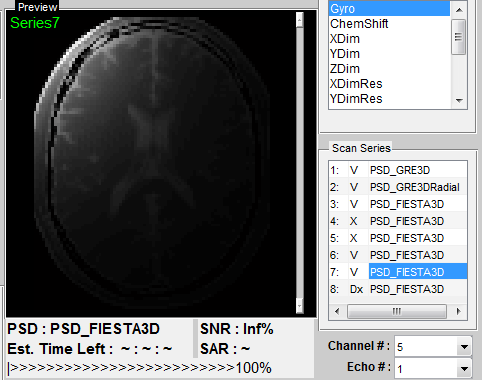
\includegraphics[width=1\textwidth]{Pictures/SimulationImage2.eps}
	\caption{A Preview of A Simulated Image with Multiple Receiving. The preview is one slice of simulated image using FIESTA sequence with 8 channel head coil. The image is from the fifth coil channel.}
	\label{fig:SimulationImage2}
\end{figure}

At the bottom of the preview axes, there are information for the name of currently running sequence, estimated remaining scan time in real time and a scan progress bar. A global relative SNR and SAR (:TODO) are also provided and automatic updated in real time. The relative SNR is defined as the ratio of current SNR to the initial SNR calculated upon loading the sequence. The SNR value is calculated using Equation \ref{eq:SNR}.

\begin{equation}
SNR = B0 \times RFreq \times RPhase \times RSlice \times \frac{\sqrt{ResFreq \times ResPhase \times SliceNum \times NEX}}{NoiseLevel \times \sqrt{BandWidth}}
\label{eq:SNR}
\end{equation}

where

\begin{equation}
\begin{aligned}
	RFreq  = \frac{FOVFreq}{ResFreq}; \\
	RPhase = \frac{FOVPhase}{ResPhase}; \\
	RSlice = SliceThick. \\
\label{eq:SNR2}
\end{aligned}
\end{equation}

In order to simulate image noise, MRiLab performs a noise adding process in K-Space after signal acquisition. The Gaussian noise with zero mean and user-defined standard deviation is added to the complex signal. The standard deviation is determined using Equation \ref{eq:Noise}. If no noise is desired, the user can set `NoiseLevel' to zero to get infinite SNR.

\begin{equation}
Noise = \frac{\frac{NoiseLevel}{NoiseRef} \times \sqrt{\frac{BandWidth}{BWRef}}}{\frac{B0}{B0Ref} \times \frac{RFreq \times RPhase \times RSlice}{VolRef}
				\times \sqrt{\frac{NEX}{NEXRef} \times \frac{ResFreq \times ResPhase \times SliceNum}{ADCRef}}}
\label{eq:Noise}
\end{equation}

where these reference values are given as:

\begin{equation}
\begin{aligned}
	BWRef  = 1e3; \\
	NoiseRef = 1; \\
	B0Ref  = 1.5; \\
  VolRef = 1e-9; \\
	NEXRef = 1; \\
	ADCRef = 1e4. \\
\label{eq:Noise2}
\end{aligned}
\end{equation}

\chapter{MRiLab Toolboxes} \label{chap:MRiLabToolboxes}

MRiLab toolboxes consists of several individual graphical user interfaces for conducting RF pulse design, MR sequence design and Coil design etc. These toolboxes allow users to fast and effectively build and customize their own specific MR simulation experiment. This chapter covers the introduction to each toolbox and corresponding macro libraries.

\section{RF Pulse Design}

The RF pulse design toolbox can be activated by pressing `RF Design Panel' toolbar icon located at the top of the main simulation console.

\begin{figure}[htbp]
	\centering
		
\includegraphics[width=0.08\textwidth]{Pictures/RFDesignPanelIcon.eps}
	\caption{RF Design Panel Toolbar Icon}
	\label{fig:RFDesignPanelIcon}
\end{figure}

\subsection{RF Design GUI}

\begin{figure}[htbp]
	\centering
		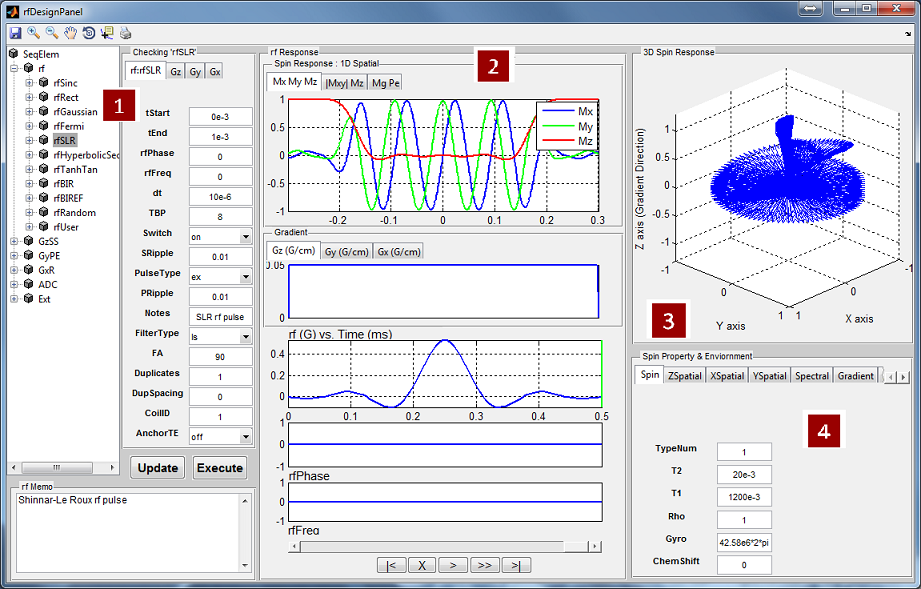
\includegraphics[width=1\textwidth]{Pictures/RFDesignGUI.eps}
	\caption{RF Design Panel. An example of simulating the slice profile of a linear phase Shinnar-Le Roux RF pulse.}
	\label{fig:RFDesignGUI}
\end{figure}

Figure \ref{fig:RFDesignGUI} demonstrates an overview of the RF Pulse Design interface. This interface consists of 


\begin{enumerate}
	\item RF and Gradient Pulse Macro Library \\

The user can use this interface to analyze tissue spin response regarding a selected RF and gradient pulse. To select a RF pulse macro, the user needs to click the macro library tree to unfold the tree structure, and then click a desired RF macro. The properties of the chosen RF macro will show on the left panel under `rf:rf name' tab. The RF memo information is also shown at the `rf Memo' panel below the tree structure. The user can press `Execute' button to start analysis process. MRiLab supports three analysis modes for analyzing 1D spatial RF pulse, 2D spatial RF pulse and Spatial-Spectral RF pulse:

\begin{itemize}
	\item 1D Spatial Mode
	
MRiLab assumes a gradient is applied in the Z direction, therefore a constant gradient will be applied if `Gz' tab is empty (Figure \ref{fig:ConstantGradient}). To select a `Gz' gradient, the user needs to choose a gradient macro under `GzSS'. For example, the `GzSelective' is a recommended gradient macro typically used for performing slice selection in MRiLab. Once the user selected a gradient macro, the `Gz:gradient name' tab will become activated and the properties of this gradient macro become accessible and editable. The user can modify macro attributes to meet design goals. To make any modification effective, the user must press `Update' button before executing the slice profile analysis. Although the library tree contains macros for another gradient line (e.g. GyPE, GxR), they are typically ignored in this mode.
	\item 2D Spatial Mode

MRiLab assumes a gradient is applied in both the X and Y directions, a constant gradient will be applied if `Gx' tab or `Gy' tab is empty. The user can choose any Gx and Gy gradient macros for these two tabs and modify macro attributes to satisfy 2D rf pulse design. To activate 2D pulse analysis, the `Spat\_Flag' under `XSpatial' tab has to be turned on (\ref{it:XSpatial}). The Gz gradient is typically ignored under this mode.

	\item Spatial-Spectral Mode
	
MRiLab assumes a gradient is applied in the Z direction, a constant gradient will be applied if `Gz' tab is empty. The user can choose any Gz gradient macros for this tab and modify macro attributes to satisfy Spatial-Spectral pulse design. The user can also modify the frequency range and resolution under `Spectral' tab (\ref{it:Spectral}). To activate Spatial-Spectral pulse analysis, the `Freq\_Flag' has to be turned on (\ref{it:Spectral}). The Gx and Gy gradient are typically ignored under this mode.

\end{itemize}

	\begin{figure}[htbp]
	\centering
		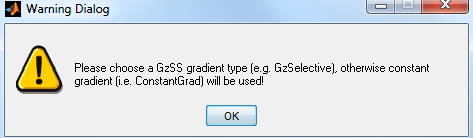
\includegraphics[width=0.8\textwidth]{Pictures/ConstantGradient.eps}
	\caption{A Warning Window for Using Constant Gradient}
	\label{fig:ConstantGradient}
\end{figure}

	\item Spin Response \\

\begin{figure}[htbp]
	\centering
		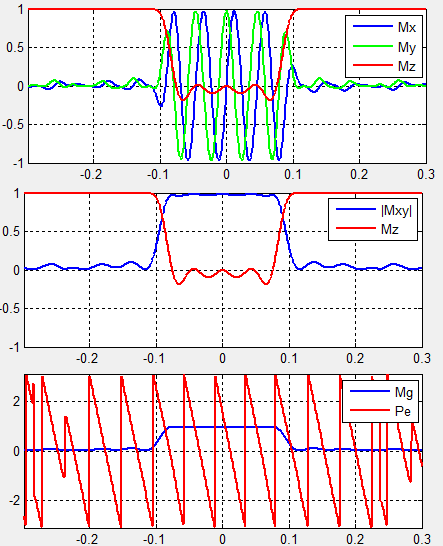
\includegraphics[width=0.8\textwidth]{Pictures/SliceProfile.eps}
	\caption{A Slice Profile Analysis of A linear phase SLR Pulse}
	\label{fig:SliceProfile}
\end{figure}

Under 1D Spatial Mode, MRiLab provides three slice profile figures (Figure \ref{fig:SliceProfile}) on the `Spin Response' panel under different tabs. These figures include slice profile regarding 

\begin{itemize}
	\item Mx My Mz : three independent spin component
	\item $\vert$Mxy$\vert$ Mz : transverse and longitudinal component
	\item Mg Pe : transverse component magnitude and phase
\end{itemize}

The horizontal axis is the spin position in units of meters, and the vertical axis is the value of the components in normalized units. 

Under 2D Spatial or Spatial-Spectral Mode, MRiLab provides another five spin response figures on the `Spin Response' panel under different tabs. These figures include

\begin{itemize}
	\item Mx : spin X component
	\item My : spin Y component
	\item Mz : spin Z component
	\item Mag : transverse component magnitude
	\item Ph : transverse component phase
\end{itemize}

The horizontal axis is the spin position for 2D Spatial mode and the frequency range for Spatial-Spectral mode, and the vertical axis is the spin location in both mode. Notice the units of both axes use spin index for either spatial position or frequency position according to spin property and environment (\ref{it:XSpatial}, \ref{it:YSpatial} and \ref{it:Spectral}). 

MRiLab also plots the RF and gradient waveform. In MRiLab, the property of a RF pulse contains RF amplitude (T), RF phase (rad) and RF frequency (Hz). The RF frequency is defined as the spin Larmor frequency minus the laboratory frequency of the RF pulse. Notice that in those figures, for display purpose, the gradient amplitude is in units of G/cm and RF amplitude is in units of G. Both time axes are in units of milliseconds. At the bottom of this interface, there is a group of pushbuttons (Figure \ref{fig:PlaybackButtonGroup}) allowing the user to investigate intermediate spin response during a applied RF and gradient (Figure \ref{fig:SliceProfileAtMiddle}). 

\begin{figure}[htbp]
	\centering
		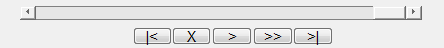
\includegraphics[width=0.8\textwidth]{Pictures/PlaybackButtonGroup.eps}
	\caption{The Playback Control Group for Spin Response}
	\label{fig:PlaybackButtonGroup}
\end{figure}

\begin{itemize}
	\item Scroll Bar : Drag the scroll bar to any intermediate time point between beginning and end 
	\item $\vert <$ : Move to the beginning
	\item X : Pause animation, notice that the interface can only be closed while animation is paused
	\item O : Resume animation
	\item $> $ : Play at normal speed
	\item $>>$ : Play at double normal speed
	\item $> \vert$ : Move to the end
\end{itemize}

\begin{figure}[htbp]
	\centering
		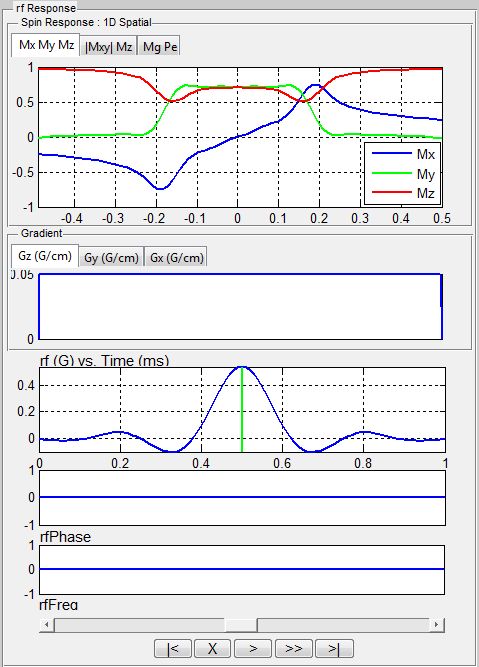
\includegraphics[width=0.8\textwidth]{Pictures/SliceProfileAtMiddle.eps}
	\caption{An Intermediate Slice Profile in The Middle of RF Pulse}
	\label{fig:SliceProfileAtMiddle}
\end{figure}

	\item 3D Spin Response \\

MRiLab renders three-dimensional spin response in `3D Spin Response' panel based on different modes. The user can inspect the behavior of spins at specific location under a chosen RF pulse and gradient. The user can use Matlab default graphical tools for interactively changing display view and size (Figure \ref{fig:MatlabDefaultTools}). To change three-dimensional spin response content reflecting different tabs in 2D spatial mode or Spatial-Spectral model (Figure \ref{fig:SpatialSpectral}), the trick is to simply activate any item of the playback control group (e.g. click the scroll bar).

\begin{figure}[htbp]
	\centering
		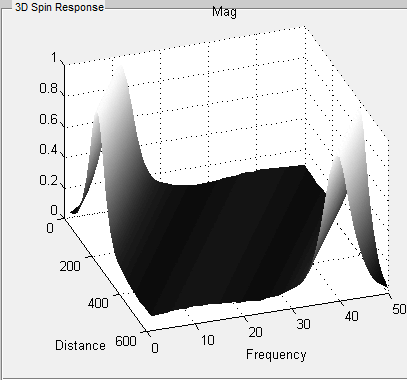
\includegraphics[width=0.6\textwidth]{Pictures/SpatialSpectral.eps}
	\caption{The Magnitude of Spin Transverse Component from A Spatial-Spectral Analysis of An Inversion Adiabatic rf Pulse}
	\label{fig:SpatialSpectral}
\end{figure}

\begin{figure}[htbp]
	\centering
		
\includegraphics[width=0.25\textwidth]{Pictures/MatlabDefaultTools.eps}
	\caption{Matlab Default Graphical Tools}
	\label{fig:MatlabDefaultTools}
\end{figure}

\item Spin Property and Environment \\

The user can modify the spin properties and environment to satisfy their experiment design. The editable properties provided in this interface include:

\begin{enumerate}

\item Spin
\begin{itemize}
	\item ChemShift (Hz/T): The chemical shift of the spin
	\item Gyro (rad/s/T): The gyromagnetic ratio of the spin
	\item Rho : The spin density of the spin
	\item T1 (s): The longitudinal relaxation time
	\item T2 (s): The transverse relaxation time
	\item TypeNum : The number of spin species
\end{itemize}

\item ZSpatial \label{it:ZSpatial}
\begin{itemize}
	\item ZCenter : The index of the centeral spin in Z direction
	\item ZSpin : The number of the spins in Z direction
	\item ZSpinGap (m): The distance between adjacent spins in Z direction
\end{itemize}

\item XSpatial \label{it:XSpatial}

\begin{itemize}
	\item XCenter : The index of the centeral spin in X direction
	\item XSpin : The number of the spins in X direction
	\item XSpinGap (m): The distance between adjacent spins in X direction
	\item Spat\_Flag: The flag to turn on and off 2D spatial rf analysis
\end{itemize}

\item YSpatial \label{it:YSpatial}

\begin{itemize}
	\item YCenter : The index of the centeral spin in Y direction
	\item YSpin : The number of the spins in Y direction
	\item YSpinGap (m): The distance between adjacent spins in Y direction
\end{itemize}

\item Spectral \label{it:Spectral}

\begin{itemize}
	\item FreqRes : The number of linear frequency sample points
	\item FreqUpLimit : The upper limit of frequency range
	\item FreqDownLimit : The lower limit of frequency range
	\item Freq\_Flag: The flag to turn on and off Spatial-Spectral rf analysis
\end{itemize}

\item Gradient

\begin{itemize}
	\item ConstantGrad (T/m): The constant gradient applied when gradient tab is empty
\end{itemize}

\item Magnet

\begin{itemize}
	\item dB0 (T): The main magnetic field offset
\end{itemize}

\end{enumerate}

\begin{figure}[htbp]
	\centering
		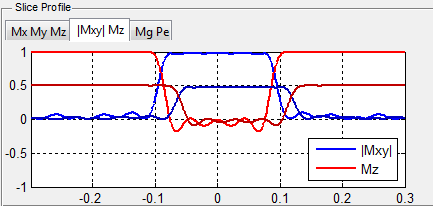
\includegraphics[width=0.8\textwidth]{Pictures/SliceProfileTwoSpecies.eps}
	\caption{A Slice Profile Analysis of Two Spin Species}
	\label{fig:SliceProfileTwoSpecies}
\end{figure}

Figure \ref{fig:SliceProfileTwoSpecies} demonstrates a slice profile for two different spin species under the same RF pulse and gradient in 1D spatial mode. To enable slice profile analysis for multiple spin species, the user needs to provide multiple values for T1, T2, Rho and ChemShift in an array, and give the correct number of spin species. The values must be separated with space. For example

\begin{itemize}
	\item ChemShift = 0 -210
	\item Rho = 1.0 0.5
	\item T1 = 1.2 1.0
	\item T2 = 0.02 0.03
	\item TypeNum = 2
\end{itemize}

\end{enumerate}

\subsection{RF Macro Library}

MRiLab uses a concept of macros for simplifying experiment design. A RF macro is a predefined module for a RF pulse with the features of programming-free and flexible of modification for specific experimental design using the RF Design interface. MRiLab RF macro library is a collection of RF macros covering from simple RF pulses such as hard pulse, to complex RF pulses such as adiabatic pulses. A specific RF macro to interact with external RF pulse file is also provided to create more extensible pulse design environment. This section will give an introduction to each of the RF macros provided in MRiLab.

\subsubsection{rfSinc}

A RF macro that creates a Sinc type RF pulse. This macro contains attributes including:

\begin{itemize}
	\item Apod : Apodization methods including `Non', `Hamming' and `Hanning'
	\item FA (Degree) : Prescribed flip angle 
	\item TBP : The time bandwidth product
	\item dt (s) : The time interval of RF pulse sample points
	\item rfPhase (rad) : RF pulse phase
	\item rfFreq (Hz) : RF pulse frequency
	\item tStart (s) : RF pulse starting time
	\item tEnd (s) : RF pulse ending time
	\item Switch : The flag for turning on and off RF pulse in the RF sequence line
	\item AnchorTE : The flag for turning on and off TE reference, TE is calculated from this RF pulse if this flag is turned on
	\item Duplicates : The number of the RF pulse duplicates, used for creating multiple RF pulses with the same shape
	\item DupSpacing : The time spacing between RF pulse duplicates
	\item CoilID : The ID of the coil element used with this RF pulse, applied for multiple RF transmitting
	\item Notes : The notes of the RF pulse 
\end{itemize}

The time dependence of the Sinc RF pulse is given by \cite{Handbook2004}:

\begin{equation}
B_1(t) = 
\begin{cases}
 A t_0 \frac{sin(\frac{\pi t}{t_0})}{\pi t} &  -N_L t_0 \leq t \leq N_R t_0 \\
 0                                          &  \text{elsewhere}
\end{cases}
\label{eq:Sinc}
\end{equation}

where $A$ is the peak RF amplitude automatically calculated and scaled according to flip angle, $t_0$ is one-half the width of the central lobe, and the $N_L$ and $N_R$ are the number of zero-crossings to the left and right of the central peak, respectively. In MRiLab, the $N_L \equiv N_R$, thus the Sinc RF pulse is always symmetric. Notice that the The time bandwidth product of a Sinc pulse equals the number of zero-crossings including the start and end. In order to address the discontinuity at the start and end, apodization can be applied using `Hamming' or `Hanning' window as described by:

\begin{equation}
Apodization(t) = 
\begin{cases}
 (1-\alpha) + \alpha cos(\frac{\pi t}{N t_0}) &  -N_L t_0 \leq t \leq N_R t_0 \\
 0                                          &  \text{elsewhere}
\end{cases}
\label{eq:Apodization}
\end{equation}

where $N$ equals $N_L$ and $N_R$. Hamming window uses $\alpha=0.46$, and Hanning window uses $\alpha=0.5$. If `Non' is used, apodization is disabled.

\subsubsection{rfRect}

A RF macro that creates a hard RF pulse. This macro contains attributes including:

\begin{itemize}
	\item FA (Degree) : Prescribed flip angle 
	\item dt (s) : The time interval of RF pulse sample points
	\item rfPhase (rad) : RF pulse phase
	\item rfFreq (Hz) : RF pulse frequency
	\item tStart (s) : RF pulse starting time
	\item tEnd (s) : RF pulse ending time
	\item Switch : The flag for turning on and off RF pulse in the RF sequence line
	\item AnchorTE : The flag for turning on and off TE reference, TE is calculated from this RF pulse if this flag is turned on
	\item Duplicates : The number of the RF pulse duplicates, used for creating multiple RF pulses with the same shape
	\item DupSpacing : The time spacing between RF pulse duplicates
	\item CoilID : The ID of the coil element used with this RF pulse, applied for multiple RF transmitting
	\item Notes : The notes of the RF pulse 
\end{itemize}


The time dependence of the hard RF pulse is given by \cite{Handbook2004}:

\begin{equation}
B_1(t) = 
\begin{cases}
 A  &  |t| \leq \frac{T}{2} \\
 0  &  |t| > \frac{T}{2}
\end{cases}
\label{eq:Rect}
\end{equation}

where $A$ is the peak RF amplitude automatically calculated and scaled according to flip angle, $T$ is the width of RF pulse that equals tEnd-tStart.

\subsubsection{rfGaussian}

A RF macro that creates a Gaussian type RF pulse. This macro contains attributes including:

\begin{itemize}
	\item FA (Degree) : Prescribed flip angle 
	\item dt (s) : The time interval of RF pulse sample points
	\item rfPhase (rad) : RF pulse phase
	\item rfFreq (Hz) : RF pulse frequency
	\item tStart (s) : RF pulse starting time
	\item tEnd (s) : RF pulse ending time
	\item Switch : The flag for turning on and off RF pulse in the RF sequence line
	\item AnchorTE : The flag for turning on and off TE reference, TE is calculated from this RF pulse if this flag is turned on
	\item Duplicates : The number of the RF pulse duplicates, used for creating multiple RF pulses with the same shape
	\item DupSpacing : The time spacing between RF pulse duplicates
	\item CoilID : The ID of the coil element used with this RF pulse, applied for multiple RF transmitting
	\item Notes : The notes of the RF pulse 
\end{itemize}

The time dependence of the Gaussian RF pulse is given by \cite{Handbook2004}:

\begin{equation}\
B_1(t) = A e^{-\frac{t^2}{2 \sigma ^2}} \quad \text{pulse centered at } t = 0
\label{eq:Gaussian}
\end{equation}

where $A$ is the peak RF amplitude automatically calculated and scaled according to flip angle, $\sigma$ is linearly proportional to the pulse width. Also the Gaussian RF pulse is terminated with a 60-dB attenuation.

\subsubsection{rfFermi}

A RF macro that creates a Fermi RF pulse. This macro contains attributes including:

\begin{itemize}
	\item PW : The measure of the pulse width
	\item FA (Degree) : Prescribed flip angle 
	\item dt (s) : The time interval of RF pulse sample points
	\item rfPhase (rad) : RF pulse phase
	\item rfFreq (Hz) : RF pulse frequency
	\item tStart (s) : RF pulse starting time
	\item tEnd (s) : RF pulse ending time
	\item Switch : The flag for turning on and off RF pulse in the RF sequence line
	\item AnchorTE : The flag for turning on and off TE reference, TE is calculated from this RF pulse if this flag is turned on
	\item Duplicates : The number of the RF pulse duplicates, used for creating multiple RF pulses with the same shape
	\item DupSpacing : The time spacing between RF pulse duplicates
	\item CoilID : The ID of the coil element used with this RF pulse, applied for multiple RF transmitting
	\item Notes : The notes of the RF pulse 
\end{itemize}

The time dependence of the Fermi RF pulse is given by \cite{Handbook2004}:

\begin{equation}\
B_1(t) = \frac{A}{1+e^{\frac{|t|-t_0}{\alpha}}} \quad \text{pulse centered at } t = 0
\label{eq:Fermi}
\end{equation}

where $A$ is the peak RF amplitude automatically calculated and scaled according to flip angle, $t_0$ is a measure of the pulse width that corresponds to PW, $\alpha$ is a measure of the transition width. The Fermi pulse approximates more to a rectangle pulse with larger $t_0$ value. Also the Fermi RF pulse is terminated with a 60-dB attenuation.

\subsubsection{rfSLR}

A RF macro that creates a RF pulse using Shinnar-Le Roux algorithm. This macro contains attributes including:

\begin{itemize}
	\item PulseType : The type of this SLR pulse, including `st' (small tip angle pulse), `ex' (excitation pulse), `se' (spin-echo pulse), `sat' (saturation pulse) and `inv' (inversion pulse)
	\item FilterType : The type of the applied filter design method, including `ls' (least squares), `min' (minimum phase), `max' (maximum phase), `pm' (Parks-McClellan equal ripple), and `ms' (Hamming windowed sinc)
	\item PRipple : The ripple factor at passband
	\item SRipple : The ripple factor at stopband
	\item FA (Degree) : Prescribed flip angle 
	\item TBP : The time bandwidth product
	\item dt (s) : The time interval of RF pulse sample points
	\item rfPhase (rad) : RF pulse phase
	\item rfFreq (Hz) : RF pulse frequency
	\item tStart (s) : RF pulse starting time
	\item tEnd (s) : RF pulse ending time
	\item Switch : The flag for turning on and off RF pulse in the RF sequence line
	\item AnchorTE : The flag for turning on and off TE reference, TE is calculated from this RF pulse if this flag is turned on
	\item Duplicates : The number of the RF pulse duplicates, used for creating multiple RF pulses with the same shape
	\item DupSpacing : The time spacing between RF pulse duplicates
	\item CoilID : The ID of the coil element used with this RF pulse, applied for multiple RF transmitting
	\item Notes : The notes of the RF pulse 
\end{itemize}

MRiLab implements a library of Matlab SLR pulse design routines that is originally developed by Prof. John Pauly and published online at \url{http://rsl.stanford.edu/research/software.html}. Thorough explanation of the algorithm is beyond the scope of this manual, users who are interested in the SLR algorithm are referred to \cite{Handbook2004,Pauly1991}.


\subsubsection{rfHyperbolicSecant}

A RF macro that creates an adiabatic inversion RF pulse based on hyperbolic secant modulation. This macro contains attributes including:

\begin{itemize}
	\item Adiab : The adiabatic factor
	\item MaxB1 (T) : The maximum B1 field
	\item TBP : The time bandwidth product
	\item dt (s) : The time interval of RF pulse sample points
	\item rfPhase (rad) : RF pulse phase
	\item tStart (s) : RF pulse starting time
	\item tEnd (s) : RF pulse ending time
	\item Switch : The flag for turning on and off RF pulse in the RF sequence line
	\item AnchorTE : The flag for turning on and off TE reference, TE is calculated from this RF pulse if this flag is turned on
	\item Duplicates : The number of the RF pulse duplicates, used for creating multiple RF pulses with the same shape
	\item DupSpacing : The time spacing between RF pulse duplicates
	\item CoilID : The ID of the coil element used with this RF pulse, applied for multiple RF transmitting
	\item Notes : The notes of the RF pulse 
\end{itemize}

The time dependence of the hyperbolic secant RF pulse is given by \cite{Handbook2004}:

\begin{equation}\
\begin{aligned}
A(t) = A_0 sech(\beta t) \quad \text{amplitude modulation } \\
F(t) = \frac{-\mu \beta}{2 \pi} tanh(\beta t) \quad \text{frequency modulation } \\
\end{aligned}
\label{eq:HyperbolicSecant}
\end{equation}

where $A_0$ is the maximum B1 field corresponding to MaxB1, $\mu$ is a dimensionless adiabatic factor corresponding to Adiab, $\beta$ is an modulation angular frequency. It can be shown that TBP has the relationship with $\beta$ and $\mu$ as

\begin{equation}\
TBP = \frac{T\mu \beta}{\pi}
\label{eq:TBPHyperbolicSecant}
\end{equation}

where $T$ is the pulse width.

To satisfy the Adiabatic Condition, the parameter setting has to meet 

\begin{equation}\
A_0 \gg \frac{\sqrt{\mu}\beta}{\gamma}
\label{eq:ACHyperbolicSecant}
\end{equation}

\subsubsection{rfTanhTan}

A RF macro that creates an adiabatic inversion RF pulse based on tanh/tan modulation. This macro contains attributes including:

\begin{itemize}
	\item MaxB1 (T) : The maximum B1 field
	\item TBP : The time bandwidth product
	\item dt (s) : The time interval of RF pulse sample points
	\item rfPhase (rad) : RF pulse phase
	\item tStart (s) : RF pulse starting time
	\item tEnd (s) : RF pulse ending time
	\item Switch : The flag for turning on and off RF pulse in the RF sequence line
	\item AnchorTE : The flag for turning on and off TE reference, TE is calculated from this RF pulse if this flag is turned on
	\item Duplicates : The number of the RF pulse duplicates, used for creating multiple RF pulses with the same shape
	\item DupSpacing : The time spacing between RF pulse duplicates
	\item CoilID : The ID of the coil element used with this RF pulse, applied for multiple RF transmitting
	\item Notes : The notes of the RF pulse 
\end{itemize}

The tanh/tan RF pulse is constructed from an adiabatic half passage and its time-reversed adiabatic half passage. The time dependence of the first adiabatic half passage is given by \cite{Hwang1998}:

\begin{equation}\
\begin{aligned}
A(t) = \gamma A_0 tanh(\frac{2 \xi t}{T}) \quad 0 \leq t \leq \frac{T}{2} \quad \text{amplitude modulation } \\
F(t) = A \frac{tan(\kappa (1-\frac{2t}{T}))}{2 \pi tan(\kappa)} \quad 0 \leq t \leq \frac{T}{2} \quad \text{frequency modulation } \\
\end{aligned}
\label{eq:TanhTan}
\end{equation}

where $A_0$ is the maximum B1 field corresponding to MaxB1, $\xi = 10$, $tan(\kappa) = 20$, $T$ is the pulse width. The TBP can be estimated using

\begin{equation}\
TBP = \frac{A\cdot T}{\pi}
\label{eq:TBPTanhTan}
\end{equation}


\subsubsection{rfBIR}

A RF macro that creates an adiabatic B1 Independent Rotation (BIR) RF pulse. This macro contains attributes including:

\begin{itemize}
	\item MaxB1 (T) : The maximum B1 field
	\item MaxFreq (Hz) : The maximum RF frequency
	\item Lambda : The $\lambda$ adiabatic factor
	\item Beta : The $\beta$ adiabatic factor
	\item BIRFlag : The type of BIR pulse, including `BIR-1', `BIR-2' and `BIR-4'
	\item dt (s) : The time interval of RF pulse sample points
	\item tStart (s) : RF pulse starting time
	\item tEnd (s) : RF pulse ending time
	\item Switch : The flag for turning on and off RF pulse in the RF sequence line
	\item AnchorTE : The flag for turning on and off TE reference, TE is calculated from this RF pulse if this flag is turned on
	\item Duplicates : The number of the RF pulse duplicates, used for creating multiple RF pulses with the same shape
	\item DupSpacing : The time spacing between RF pulse duplicates
	\item CoilID : The ID of the coil element used with this RF pulse, applied for multiple RF transmitting
	\item Notes : The notes of the RF pulse 
\end{itemize}

The time dependence of the BIR-1 RF pulse is given by \cite{Handbook2004}: \\
Amplitude modulation:
\begin{equation}
A(t) = 
\begin{cases}
 \hat{x} A_0 cos(\xi t)  &  0 \leq t < \frac{T}{2} \\
 \hat{y} A_0 cos(\xi t)  &  \frac{T}{2} \leq t \leq T
\end{cases}
\label{eq:BIR1A}
\end{equation}
\\
Frequency modulation:
\begin{equation}
F(t) = 
\begin{cases}
  F_0 sin(\xi t)  &  0 \leq t < \frac{T}{2} \\
 - F_0 sin(\xi t)  &  \frac{T}{2} \leq t \leq T
\end{cases}
\label{eq:BIR1F}
\end{equation}

where $A_0$ is the maximum B1 field corresponding to MaxB1, $F_0$ is the maximum RF frequency corresponding to MaxFreq. The RF pulse width is $T = \frac{\pi}{\xi}$, and $\hat{x}$ and $\hat{y}$ are unit vectors for indicating RF phase. \\

The time dependence of the BIR-2 RF pulse is given by \cite{Handbook2004}: \\
Amplitude modulation:
\begin{equation}
A(t) = 
\begin{cases}
 \hat{x} |A_0 cos(\xi t)|  &  0 \leq t < \frac{T}{2} \\
 \hat{y} |A_0 cos(\xi t)|  &  \frac{T}{2} \leq t < T \\
 -\hat{y} |A_0 cos(\xi t)|  &  T \leq t \leq 2T
\end{cases}
\label{eq:BIR2A}
\end{equation}
\\
Frequency modulation:
\begin{equation}
F(t) = |F_0 sin(\xi t)|
\label{eq:BIR2F}
\end{equation}

where $A_0$ is the maximum B1 field corresponding to MaxB1, $F_0$ is the maximum RF frequency corresponding to MaxFreq. The RF pulse width is $T = \frac{\pi}{\xi}$, and $\hat{x}$ and $\hat{y}$ are unit vectors for indicating RF phase. \\

The time dependence of the BIR-4 RF pulse is given by \cite{Handbook2004}: \\
Amplitude modulation:
\begin{equation}
A(t) = 
\begin{cases}
 A_0 tanh[\lambda (1-\frac{4t}{T})]  &  0 \leq t < \frac{T}{4} \\
 A_0 tanh[\lambda (\frac{4t}{T}-1)]  &  \frac{T}{4} \leq t < \frac{T}{2}\\
 A_0 tanh[\lambda (3-\frac{4t}{T})]  &  \frac{T}{2} \leq t < \frac{3T}{4} \\
 A_0 tanh[\lambda (\frac{4t}{T}-3)]  &  \frac{3T}{4} \leq t \leq T
\end{cases}
\label{eq:BIR4A}
\end{equation}
\\
Frequency modulation:
\begin{equation}
F(t) =
\begin{cases}
 \frac{tan(\frac{4\beta t}{T})}{tan(\beta)}  &  0 \leq t < \frac{T}{4} \\
 \frac{tan[\beta (\frac{4t}{T}-2)]}{tan(\beta)}  &  \frac{T}{4} \leq t < \frac{T}{2}\\
 \frac{tan[\beta (\frac{4t}{T}-2)]}{tan(\beta)}   &  \frac{T}{2} \leq t < \frac{3T}{4} \\
 \frac{tan[\beta (\frac{4t}{T}-4)]}{tan(\beta)}   &  \frac{3T}{4} \leq t \leq T
\end{cases}
\label{eq:BIR4F}
\end{equation}

where $A_0$ is the maximum B1 field corresponding to MaxB1. The RF pulse width is $T$. The $\lambda$ and $\beta$ are dimensionless constants that describe the degree to which extent the RF pulse satisfies the adiabatic condition.


\subsubsection{rfBIREF}

A RF macro that creates an adiabatic B1 Independent Refocusing (BIREF) RF pulse. This macro contains attributes including:

\begin{itemize}
	\item MaxB1 (T) : The maximum B1 field
	\item MaxFreq (Hz) : The maximum RF frequency
	\item BIREFFlag : The type of BIREF pulse, including `BIREF-1', `BIREF-2a' and `BIREF-2b'
	\item dt (s) : The time interval of RF pulse sample points
	\item tStart (s) : RF pulse starting time
	\item tEnd (s) : RF pulse ending time
	\item Switch : The flag for turning on and off RF pulse in the RF sequence line
	\item AnchorTE : The flag for turning on and off TE reference, TE is calculated from this RF pulse if this flag is turned on
	\item Duplicates : The number of the RF pulse duplicates, used for creating multiple RF pulses with the same shape
	\item DupSpacing : The time spacing between RF pulse duplicates
	\item CoilID : The ID of the coil element used with this RF pulse, applied for multiple RF transmitting
	\item Notes : The notes of the RF pulse 
\end{itemize}

The time dependence of the BIREF-1 RF pulse is given by \cite{Handbook2004}: \\
Amplitude modulation:
\begin{equation}
A(t) = 
\begin{cases}
 \hat{x} A_0 sin(\xi t)  &  0 \leq t < \frac{T}{2} \\
 -\hat{x} A_0 sin(\xi t)  &  \frac{T}{2} \leq t \leq T
\end{cases}
\label{eq:BIREF1A}
\end{equation}
\\
Frequency modulation:
\begin{equation}
F(t) = F_0 |cos(\xi t)|
\label{eq:BIREF1F}
\end{equation}

where $A_0$ is the maximum B1 field corresponding to MaxB1, $F_0$ is the maximum RF frequency corresponding to MaxFreq. The RF pulse width is $T = \frac{\pi}{\xi}$, and $\hat{x}$ is an unit vector for indicating RF phase along the $x$ axis. \\

The time dependence of the BIREF-2a RF pulse is given by \cite{Handbook2004}: \\
Amplitude modulation:
\begin{equation}
A(t) = \hat{x} A_0 |cos(\xi t)|
\label{eq:BIREF2aA}
\end{equation}
\\
Frequency modulation:
\begin{equation}
F(t) = 
\begin{cases}
 F_0 sin(\xi t)  &  0 \leq t < \frac{T}{2} \\
 -F_0 sin(\xi t)  &  \frac{T}{2} \leq t \leq T
\end{cases}
\label{eq:BIREF2aF}
\end{equation}

where $A_0$ is the maximum B1 field corresponding to MaxB1, $F_0$ is the maximum RF frequency corresponding to MaxFreq. The RF pulse width is $T = \frac{\pi}{\xi}$, and $\hat{x}$ is an unit vector for indicating RF phase along the $x$ axis. \\

The time dependence of the BIREF-2b RF pulse is given by \cite{Handbook2004}: \\
Amplitude modulation:
\begin{equation}
A(t) = 
\begin{cases}
 \hat{x} A_0 |cos(\xi t)|  &  0 \leq t < \frac{T}{2} \\
 -\hat{x} A_0 cos(\xi t)  &  \frac{T}{2} \leq t \leq T
\end{cases}
\label{eq:BIREF2bA}
\end{equation}
\\
Frequency modulation:
\begin{equation}
F(t) = 
\begin{cases}
 F_0 sin(\xi t)  &  0 \leq t < \frac{T}{4} \\
 -F_0 sin(\xi t)  &  \frac{T}{4} \leq t < \frac{3T}{4} \\
 F_0 sin(\xi t)  &  \frac{3T}{4} \leq t \leq T
\end{cases}
\label{eq:BIREF2bF}
\end{equation}

where $A_0$ is the maximum B1 field corresponding to MaxB1, $F_0$ is the maximum RF frequency corresponding to MaxFreq. The RF pulse width is $T = \frac{2\pi}{\xi}$, and $\hat{x}$ is an unit vector for indicating RF phase along the $x$ axis. \\

\subsubsection{rfRandom}

A RF macro that creates a RF pulse with normally distributed pseudo-random amplitude. This macro is used for program testing purpose, however it shows that almost any arbitrary RF pulse could potentially be supported by MRiLab. This macro contains attributes including:

\begin{itemize}
	\item rfGain : The standard deviation of the normal distribution
	\item dt (s) : The time interval of RF pulse sample points
	\item rfPhase (rad) : RF pulse phase
	\item rfFreq (Hz) : RF pulse frequency
	\item tStart (s) : RF pulse starting time
	\item tEnd (s) : RF pulse ending time
	\item Switch : The flag for turning on and off RF pulse in the RF sequence line
	\item AnchorTE : The flag for turning on and off TE reference, TE is calculated from this RF pulse if this flag is turned on
	\item Duplicates : The number of the RF pulse duplicates, used for creating multiple RF pulses with the same shape
	\item DupSpacing : The time spacing between RF pulse duplicates
	\item CoilID : The ID of the coil element used with this RF pulse, applied for multiple RF transmitting
	\item Notes : The notes of the RF pulse 
\end{itemize}

\subsubsection{rfUser}

If the user has the RF pulse waveform data saved in a MAT file, the user can easily import the RF file into MRiLab pulse design interface by using `rfUser' macro. The RF pulse MAT file needs to contain four matrices including `rfTime' (i.e. RF time points) , `rfAmp' (i.e. RF amplitude), `rfPhase' (i.e. RF phase) and `rfFreq' (i.e. RF frequency). All four matrices must have the same size of m-by-n, where m is the number of TR sections and n is the number of RF waveform points. In typical MR sequence, the entire sequence is composed of multiple TR sections. The $i$th TR section uses the $i$th RF pulse stored in the $i$th row of these four matrices. If the number of row is less than the number of TR sections, the last RF pulse will be used for all the remaining TR sections. Notice that if `rfPhase' and/or `rfFreq' are not provided, MRiLab initializes them as a value of 0. However, `rfTime' and `rfAmp' must be provided. Also note that MRiLab only uses the first RF pulse in the MAT file for pulse analysis in the RF pulse design interface. The `rfUser' macro contains attributes including:

\begin{itemize}
	\item rfFile : The path to the file that stores the RF pulse data, quoted using single quotes
	\item Switch : The flag for turning on and off RF pulse in the RF sequence line
	\item AnchorTE : The flag for turning on and off TE reference, TE is calculated from this RF pulse if this flag is turned on
	\item Duplicates : The number of the RF pulse duplicates, used for creating multiple RF pulses with the same shape
	\item DupSpacing : The time spacing between RF pulse duplicates
	\item CoilID : The ID of the coil element used with this RF pulse, applied for multiple RF transmitting
	\item Notes : The notes of the RF pulse 
\end{itemize}

\subsection{Make New RF Macro}

The RF pulse macro library covers several common types of RF pulse waveform. However, comprehensive coverage of existing and under developed RF pulses is nearly impossible for almost any pulse sequence design tools. To address this problem in MRiLab, the user can use the `rfUser' to import RF pulses from files that are generated by other programs. Another way to import RF pulse is to simply write a RF macro. To create a RF macro, the user should follow the following steps :

\begin{enumerate}

\item Write RF macro code \\

It is strongly recommended to write your own RF macro code based on the closest RF macros in the MRiLab macro library, for example, the `rfRect' macro is coded as:

\begin{verbatim}
function [rfAmp,rfPhase,rfFreq,rfCoil,rfTime]=rfRect(p)
%Create a hard RF pulse starting from tStart and ending at tEnd
%tStart RF start time
%tEnd RF end time
%FA RF actual flip angle
%dt RF sample time
%rfPhase RF phase
%rfFreq RF off-res freq

tStart=p.tStart;
tEnd=p.tEnd;
FA=p.FA;
dt=p.dt;
rfPhase=p.rfPhase;
rfFreq=p.rfFreq;
rfCoil=p.CoilID;
Duplicates=max(1,p.Duplicates);
DupSpacing=max(0,p.DupSpacing);

rfTime=linspace(tStart,tEnd,ceil((tEnd-tStart)/dt)+1);
rfAmp=ones(size(rfTime)); % Rectangle
rfAmp(1)=0;
rfAmp(end)=0;
rfAmp=DoB1Scaling(rfAmp,dt,FA)*rfAmp; %B1 Scaling

rfPhase=(rfPhase)*ones(size(rfTime));
rfFreq=(rfFreq)*ones(size(rfTime));
rfCoil=(rfCoil)*ones(size(rfTime));
rfPhase(1)=0;
rfPhase(end)=0;
rfFreq(1)=0;
rfFreq(end)=0;

% Create Duplicates
if Duplicates~=1 & DupSpacing ~=0
    rfAmp=repmat(rfAmp,[1 Duplicates]);
    rfFreq=repmat(rfFreq,[1 Duplicates]);
    rfPhase=repmat(rfPhase,[1 Duplicates]);
    rfCoil=repmat(rfCoil,[1 Duplicates]);
    TimeOffset = repmat(0:DupSpacing:(Duplicates-1)*DupSpacing, ...
                       [length(rfTime) 1]);
    rfTime=repmat(rfTime,[1 Duplicates]) + (TimeOffset(:))';
end

end
\end{verbatim}

Your macro must start from a function declaration at the beginning, then followed by attribute input section. The `tStart' and `tEnd' need to be added for indicating the time scale. It's also strongly recommended to add attribute input `rfCoil',`Duplicates' and `DupSpacing' for multi-transmitting and multi-echo support.

\begin{verbatim}
function [rfAmp,rfPhase,rfFreq,rfCoil,rfTime]=rfMacroName(p)
%Create a RF pulse based on user code

tStart=p.tStart;
tEnd=p.tEnd;
rfCoil=p.CoilID;
Duplicates=max(1,p.Duplicates);
DupSpacing=max(0,p.DupSpacing);
...
attribute1=p.attribute1;
attribute2=p.attribute2;
attribute3=p.attribute3;
...
\end{verbatim}

The main code should deal with calculation for `rfAmp', `rfPhase', `rfFreq' and `rfTime'. Notice that they should have the same size as 1-by-m where m is the number of RF waveform points.

\begin{verbatim}
% The main code for user macro
...
rfTime = ...;
rfAmp = ...;
rfPhase = ...;
rfFreq = ...;
...
\end{verbatim}


Then you should add several lines to end your macro,

\begin{verbatim}
% Avoid baseline offset
rfAmp(1)=0;
rfAmp(end)=0;
rfPhase(1)=0;
rfPhase(end)=0;
rfFreq(1)=0;
rfFreq(end)=0;

% Assign coil element index number
rfCoil=(rfCoil)*ones(size(rfTime));

% Create Duplicates
if Duplicates~=1 & DupSpacing ~=0
    rfAmp=repmat(rfAmp,[1 Duplicates]);
    rfFreq=repmat(rfFreq,[1 Duplicates]);
    rfPhase=repmat(rfPhase,[1 Duplicates]);
    rfCoil=repmat(rfCoil,[1 Duplicates]);
    TimeOffset=repmat(0:DupSpacing:(Duplicates-1)*DupSpacing, ... 
                     [length(rfTime) 1]);
    rfTime=repmat(rfTime,[1 Duplicates]) + (TimeOffset(:))';
end

\end{verbatim}

\item Register RF macro \\

The RF macro file can be located anywhere in the computer as long as the file is included in Matlab searching path, however it is recommended to save the file under /SeqElem/rf for consistent file organization. Besides a RF macro file that performs pulse generation, MRiLab also requires a memo .txt file that accompanies the RF macro with the name `rfMacroName\_Memo'. This file contains information about RF pulse description if necessary.

The customized RF macro needs to be registered in the macro library before using. To register a macro, open file `SeqElem.xml' under /SeqElem, then add one entry under $<$rf$>$ category with the proper attribute list. One example could be

\begin{verbatim}
<rfMacroName 
				AnchorTE="$2'on','off'" 
				CoilID="1" 
				DupSpacing="0" 
				Duplicates="1" 
				Switch="$1'on','off'" 
				tEnd="1e-3" 
				tStart="0" 
				Notes="A new RF macro" 
				attribute1="0" 
				attribute2="0" 
				attribute3="0" />
\end{verbatim}

Notice that in the above example, the first 7 attributes are required for MRiLab, The remaining attributes are optional based on user's choice.

\end{enumerate}

Once the RF macro is coded and registered to the library, the user can use this customized RF macro just like those default RF macros in the library.

\section{MR Sequence Design}

The MR Sequence Design toolbox can be activated by pressing `Sequence Design Panel' toolbar icon located at the top of the main simulation console. The current loaded sequence will show in the MR Sequence Design interface.

\begin{figure}[htbp]
	\centering
		
\includegraphics[width=0.08\textwidth]{Pictures/SequenceDesignPanelIcon.eps}
	\caption{Sequence Design Panel Toolbar Icon}
	\label{fig:SequenceDesignPanelIcon}
\end{figure}

\subsection{Sequence Design GUI}

\begin{figure}[htbp]
	\centering
		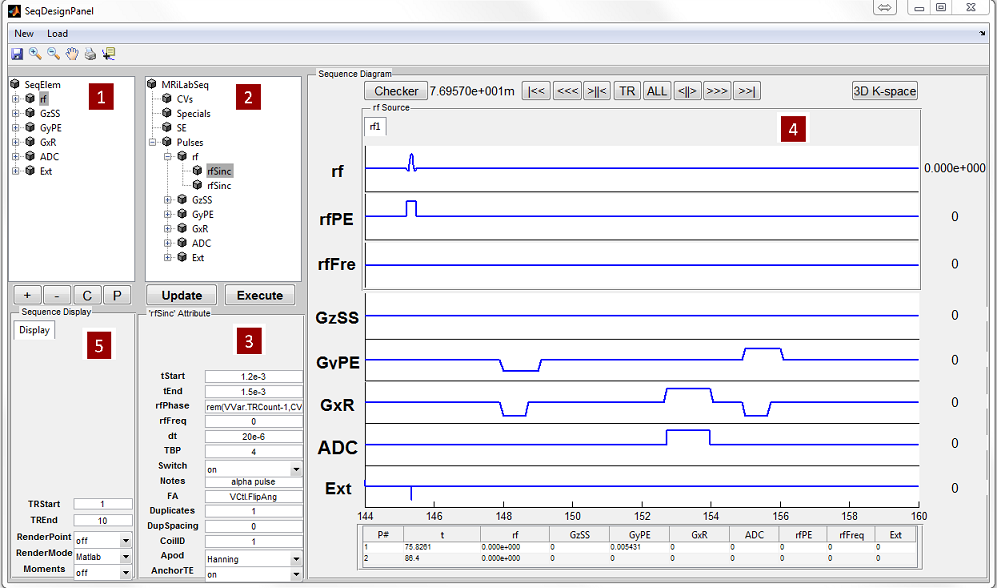
\includegraphics[width=1\textwidth]{Pictures/SequenceDesignGUI.eps}
	\caption{Sequence Design Panel. A bSSFP sequence is shown.}
	\label{fig:SequenceDesignGUI}
\end{figure}

Figure \ref{fig:SequenceDesignGUI} demonstrates an overview of the MR Sequence Design interface. This interface consists of 

\begin{enumerate}
	\item Macro Library \\
	
	The Macro Library contains a full set of pulse macros for constructing MR sequence in MRiLab. It covers not only RF macro library as described in above section, but also GzSS, GyPE and GxR gradient macro library, ADC macro library and Ext macro library. The user needs to click the `SeqElem' root as well as the subsequent nodes to unfold those macros.
	
	\item Sequence Structure \\
	
\begin{figure}[htbp]
	\centering
		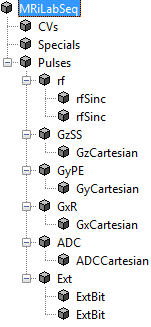
\includegraphics[width=0.3\textwidth]{Pictures/SequenceStructure.eps}
	\caption{An Example of A Typical MR Sequence Structure in MRiLab}
	\label{fig:SequenceStructure}
\end{figure}
	
	
In MRiLab, a MR sequence consists of the following parts :

\begin{itemize}
	\item CVs : The controllable variables, linked to the `CVs' tab on the main control console
	\item Specials : The applied special techniques by default
	\item SE : The starting (tS) and ending (tE) time, determining time scale for each TR section, support varying TR value
	\item Pulse
	\begin{itemize}
		\item RF : RF sequence line
		\item GzSS : GzSS sequence line
		\item GyPE : GyPE sequence line
		\item GxR : GxR sequence line
		\item ADC : Signal acquisition sequence line
		\item Ext : Extended process sequence line
	\end{itemize}
\end{itemize}

The user can construct desired MR sequence by changing the content of the MR sequence structure. To add a macro into the sequence structure, click one macro in the macro library, then click on the sequence line root (e.g. rf) to which this macro is inserted, then click `+' macro operation button. To delete a macro from the sequence structure, click the unwanted macro at the sequence line, then click `-' macro operation button. To duplicate an existing macro, first click the source macro, then click `C' macro operation button for copying, click on the sequence line root, then click `P' macro operation button for pasting. MRiLab requires the pulse macro being operated within its belonging category (e.g. RF pulse can't be added to gradient line). Also empty sequence line is prohibited.

\begin{figure}[htbp]
	\centering
		
\includegraphics[width=0.2\textwidth]{Pictures/MacroOperationButton.eps}
	\caption{Macro Operation Buttons}
	\label{fig:MacroOperationButton}
\end{figure}

	\item Pulse Attribute \\
	
Upon clicking on a pulse macro within a MR sequence structure, the corresponding macro attributes will be shown at the pulse attribute panel down below the sequence structure. The user can edit those attributes to modify the sequence waveform. To make any modification effective, the user must press `Update' button to update the associated sequence XML file. Pressing `Execute' button will update and redraw the MR sequence waveform plotting on this interface.
	
	\item Sequence Waveform \\
	
The sequence waveform associated with the sequence structure is displayed on the `Sequence Diagram' panel on the right side of this interface. The user can use the waveform diagram to inspect sequence details and layout. The sequence diagram consists of individual sequence lines corresponding to RF, GzSS, GyPE, GxR, ADC and Ext, respectively. To accommodate multiple RF transmitting, MRiLab provides separate RF sequence lines for each RF source. When `MultiTransmit' flag is turned on in the main control console and the chosen sequence structure contains multiple RF pulses for different RF sources (i.e. assign RF pulses to different coil channels by using `CoilID' attribute), the multi-tab will be activated on the `rf Source' panel (Figure \ref{fig:RFSource}). The user can switch between these tabs for checking individual RF source.

\begin{figure}[htbp]
	\centering
		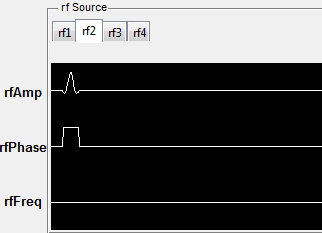
\includegraphics[width=0.6\textwidth]{Pictures/RFSource.eps}
	\caption{An Example of Multiple RF Source. The `MultiTransmit' is turned on and this sequence contains total 4 RF sources. The RF source 2 is chosen and the corresponding RF pulse waveform for coil channel 2 is shown.}
	\label{fig:RFSource}
\end{figure}

Notice that the vertical axes for all sequence lines are normalized and the horizontal axes are in units of milliseconds. MRiLab provides a group of sequence display button (Figure \ref{fig:SequenceDisplayButton}) to help inspect the sequence waveform details.

\begin{figure}[htbp]
	\centering
		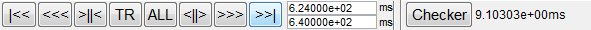
\includegraphics[width=0.8\textwidth]{Pictures/SequenceDisplayButton.eps}
	\caption{The Sequence Display Button.}
	\label{fig:SequenceDisplayButton}
\end{figure}

The sequence display button group consists of :

\begin{itemize}
	\item Checker : The time checker toggle button
	\item Time Ruler : Display current time point according to the time checker
	\item $|<<$: Move sequence waveform to the beginning
	\item $<<<$ : Move sequence waveform backwards
	\item $>||<$ : Zoom out
	\item TR : Display a sequence waveform section with a time interval of TR
	\item ALL : Display all sequence waveform
	\item $<||>$ : Zoom in
	\item $>>>$: Move sequence waveform forwards
	\item $>>|$ : Move sequence waveform to the end
\end{itemize}

The user can use the `Checker' toggle button to display a sequence waveform at any arbitrary time interval (Figure \ref{fig:AllSequence}). First press the `Checker' button, move the mouse cursor into the axes. Notice that the mouse cursor changes to a cross-hair. Move the cross-hair in the axes, the amplitude value for each sequence line will be displayed accordingly on right side of each line with their default units. The user can click on the axes to choose one side of the time slot, then click on the another side. MRiLab will change the sequence view between the chosen time points, and also save time point information in the list at the bottom of this interface. To disable `Checker' function, simple press this button again.

\begin{figure}[htbp]
	\centering
		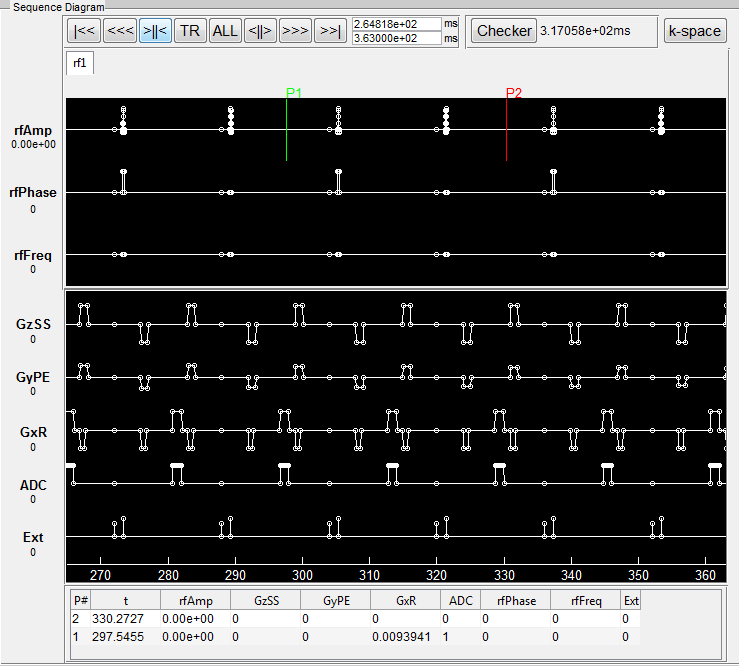
\includegraphics[width=1\textwidth]{Pictures/AllSequence.eps}
	\caption{A Sequence View with Multiple TRs.}
	\label{fig:AllSequence}
\end{figure}
	
	\item Display Control

The `Display' tab on the `Sequence Display' contains parameters for controlling sequence display and K-Space rendering.

\begin{itemize}
	\item TRStart : The first TR to be displayed
	\item TREnd : The last TR to be displayed
	\item Moments (:TODO) : The flag for turning on and off the zeroth moment display for the gradient
	\item RenderMode : The K-Space rendering mode, including `Matlab' (Figure \ref{fig:MatlabSpiral}) and `VTK' (Figure \ref{fig:VTK})
	\item RenderPoint : The flag for turning on and off K-Space point rendering
\end{itemize}	

\begin{figure}[htbp]
	\centering
		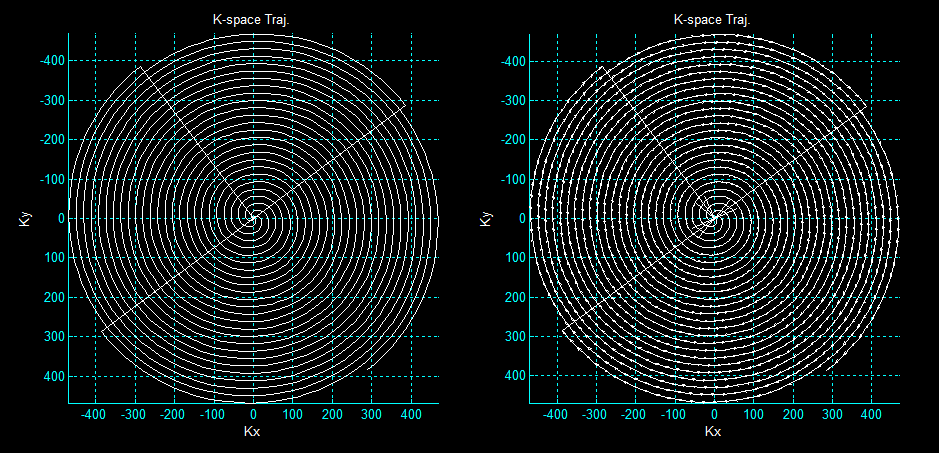
\includegraphics[width=1\textwidth]{Pictures/MatlabSpiral.eps}
	\caption{Matlab Rendered K-Space Trajectory for A Spiral Readout with 5 Interleaves. The left figure is without K-Space point rendering. The right figure is with K-Space point rendering with the arrows indicating K-Space traversing direction.}
	\label{fig:MatlabSpiral}
\end{figure}	
	
\begin{figure}[htbp]
	\centering
		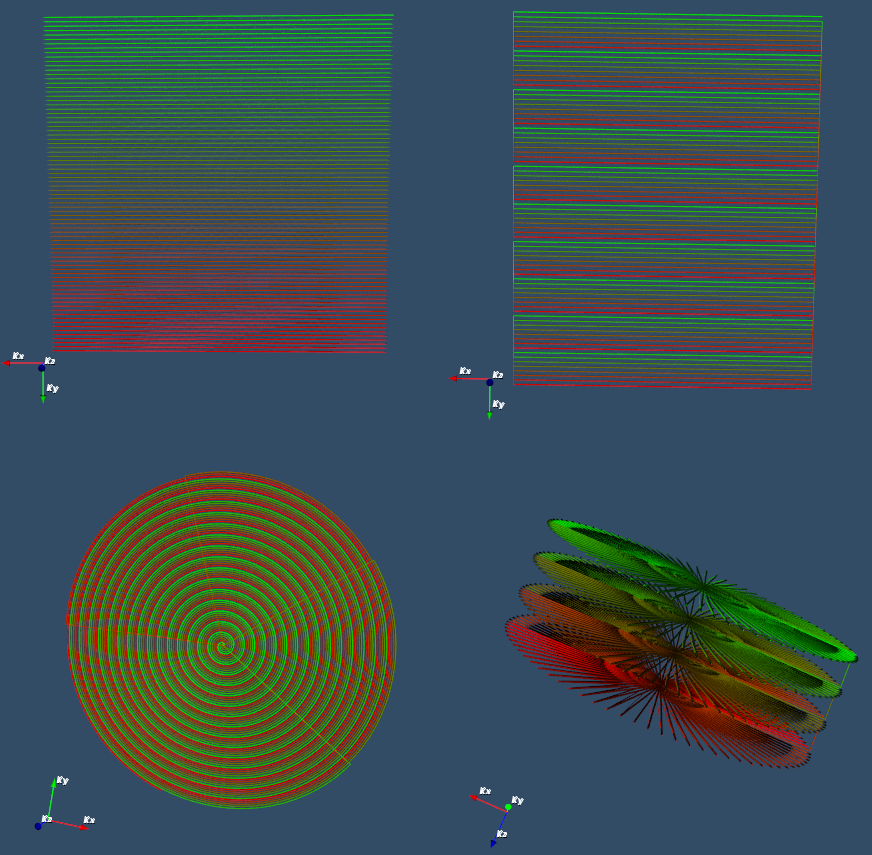
\includegraphics[width=1\textwidth]{Pictures/VTK.eps}
	\caption{VTK Rendered K-Space Trajectory Examples. The top left figure shows a typical single slice Cartesian readout. The top right figure shows a single slice multishot EPI readout. The bottom left figure shows a single slice multishot spiral readout. The bottom right figure shows a 3D Stack-of-Stars radial readout.}
	\label{fig:VTK}
\end{figure}		
	
Notice that in VTK rendering, the K-Space line color starts from green and ends to red. If the user uses VTK for K-Space rendering, please press keyboard `q' to quit the VTK window before any subsequent simulation. Pressing the quit button on the VTK window under Linux system will force the entire Matlab to close, this is `believed' to be a compatibility bug between Matlab and OpenGL which is used by VTK.

\end{enumerate}	

\subsection{Virtual Structure}
For the convenience of transferring data and configuration information across different modules, MRiLab defined several Matlab structure variables in the global scope. These structures start with `V' standing for `Virtual Structure'. Understanding what these structures are and how they are working is important to work with MRiLab and to customize specific experiment design. There are at least two virtual structures that are useful for designing MR sequences.

\begin{itemize}
	\item VCtl : Virtual Control \\
VCtl encapsules all the simulation setting parameters in the main control console. For example, the user can use `VCtl.TE' to reference `TE' value in the main control console; use `VCtl.FlipAng' to reference `FlipAng' value in the main control console. VCtl also allows the user to reference parameters in special techniques if loaded. Another example is that MRiLab uses `VCtl.TR' in the `SE' for determining time interval for each TR section. The user can use any legal Matlab syntax combined with VCtl to create desired effect, such as use `2 * VCtl.TR' to indicate twice of `TR' value.
	\item VVar : Virtual Variable \\
VVar encapsules the loop index variables that MRiLab uses for generating MR sequence waveform. A section of code for generating MR sequence is shown:

\begin{verbatim}
% MR Sequence Generating Loop
VVar.SliceCount=0;
VVar.PhaseCount=0;
VVar.TRCount=0;
s=1;
j=1;

while s<=VCtl.SecondPhNum
    VVar.SliceCount=s;
    while j<=VCtl.FirstPhNum
        VVar.PhaseCount=j;
        VVar.TRCount=VVar.TRCount+1;
				
        ...
        %Sequence Generating Code
        ...
				
        j=j+1;
    end
    j=1;
    s=s+1;
end
\end{verbatim}

The user can use the loop index variables in VVar

\begin{itemize}
	\item VVar.TRCount : The TR section index
	\item VVar.PhaseCount : The first phase encoding index
	\item VVar.SliceCount : The second (i.e. slice) phase encoding index
	\item VCtl.FirstPhNum : The total number of first phase encoding steps
	\item VCtl.SecondPhNum : The total number of second phase encoding steps
\end{itemize}	

For example, to create $180^{\circ}$ RF phase cycling in bSSFP sequence, the user can set the attributes for the excitation RF pulse as

\begin{itemize}
	\item CV3 : 2*pi/2
	\item CV4 : 2
	\item rfPhase : rem(VVar.TRCount-1,CV4)*CV3
\end{itemize}	

\end{itemize}	


\subsection{GzSS Macro Library}

A GzSS macro is a predefined module for a gradient pulse on the GzSS sequence line. MRiLab GzSS macro library is a collection of GzSS macros covering different gradient pulse types including slice selection and slice phase encoding pulses. Notice that by default the area under the gradient ramp is ignored. This section will give an introduction to each of the GzSS macros provided in MRiLab.

\subsubsection{GzSelective}

A GzSS macro that creates a typical slice selective gradient pulse (Figure \ref{fig:GzSelective}). This macro contains attributes including:

\begin{itemize}
	\item t2Start (s) : Slice selection gradient pulse starting time
	\item t2End (s) : Slice selection gradient pulse ending time
	\item tRamp (s) : Gradient pulse ramp time, assume symmetric ramp on both side
	\item GzAmp (T) : The amplitude of the gradient
	\item Gz1Sign : The polarity of the prephasing gradient, set 0 for nulling
	\item Gz2Sign : The polarity of the slice selection gradient, set 0 for nulling
	\item Gz3Sign : The polarity of the rephasing gradient, set 0 for nulling
	\item Switch : The flag for turning on and off gradient pulse in the sequence line
	\item Duplicates : The number of the gradient pulse duplicates, used for creating multiple gradient pulses with the same shape
	\item DupSpacing : The time spacing between gradient pulse duplicates
	\item Notes : The notes of the gradient pulse 
\end{itemize}

Notice that both the prephasing gradient and rephasing gradient have half of the area of the slice selection gradient.

\begin{figure}[htbp]
	\centering
		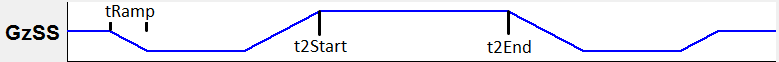
\includegraphics[width=1\textwidth]{Pictures/GzSelective.eps}
	\caption{GzSelective Waveform}
	\label{fig:GzSelective}
\end{figure}		


\subsubsection{GzSelective2}

A GzSS macro that creates a slice selective gradient pulse straddled with crusher gradient (Figure \ref{fig:GzSelective2}). This macro contains attributes including:

\begin{itemize}
	\item t2Start (s) : Slice selection gradient pulse starting time
	\item t2End (s) : Slice selection gradient pulse ending time
	\item tRamp (s) : Gradient pulse ramp time, assume symmetric ramp on both side
	\item tGz1 (s) : The duration of the left crusher
	\item tGz3 (s) : The duration of the right crusher
	\item Gz1Amp (T) : The amplitude of the left crusher
	\item Gz2Amp (T) : The amplitude of the slice selective gradient
	\item Gz3Amp (T) : The amplitude of the right crusher
	\item Switch : The flag for turning on and off gradient pulse in the sequence line
	\item Duplicates : The number of the gradient pulse duplicates, used for creating multiple gradient pulses with the same shape
	\item DupSpacing : The time spacing between gradient pulse duplicates
	\item Notes : The notes of the gradient pulse 
\end{itemize}

\begin{figure}[htbp]
	\centering
		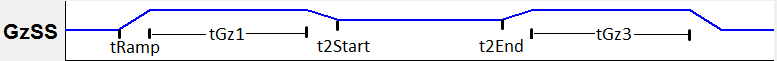
\includegraphics[width=1\textwidth]{Pictures/GzSelective2.eps}
	\caption{GzSelective2 Waveform}
	\label{fig:GzSelective2}
\end{figure}		


\subsubsection{GzTrapezoid}

A GzSS macro that creates a trapezoid gradient pulse (Figure \ref{fig:GzTrapezoid}) on GzSS sequence line. This macro contains attributes including:

\begin{itemize}
	\item tStart (s) : The trapezoid gradient pulse starting time
	\item tEnd (s) : The trapezoid gradient pulse ending time
	\item tRamp (s) : The trapezoid pulse ramp time, assume symmetric ramp on both side
	\item sRamp : The sample points on the ramp, use the value of 2 for ignoring the area under the ramp, use above 2 for counting the ramp area
	\item GzAmp (T) : The amplitude of the gradient
	\item Switch : The flag for turning on and off gradient pulse in the sequence line
	\item Duplicates : The number of the gradient pulse duplicates, used for creating multiple gradient pulses with the same shape
	\item DupSpacing : The time spacing between gradient pulse duplicates
	\item Notes : The notes of the gradient pulse 
\end{itemize}

\begin{figure}[htbp]
	\centering
		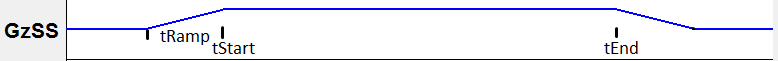
\includegraphics[width=1\textwidth]{Pictures/GzTrapezoid.eps}
	\caption{GzTrapezoid Waveform}
	\label{fig:GzTrapezoid}
\end{figure}		


\subsubsection{GzAreaTrapezoid}

A GzSS macro that creates a trapezoid gradient pulse of specified area (Figure \ref{fig:GzAreaTrapezoid}) on GzSS sequence line. This macro contains attributes including:

\begin{itemize}
	\item tStart (s) : The trapezoid gradient pulse starting time
	\item tEnd (s) : The trapezoid gradient pulse ending time
	\item Area (1/m) : The area under this gradient pulse
	\item Switch : The flag for turning on and off gradient pulse in the sequence line
	\item Duplicates : The number of the gradient pulse duplicates, used for creating multiple gradient pulses with the same shape
	\item DupSpacing : The time spacing between gradient pulse duplicates
	\item Notes : The notes of the gradient pulse 
\end{itemize}

\begin{figure}[htbp]
	\centering
		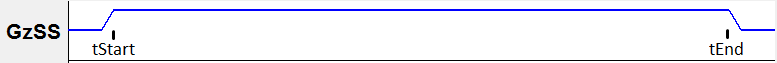
\includegraphics[width=1\textwidth]{Pictures/GzAreaTrapezoid.eps}
	\caption{GzAreaTrapezoid Waveform}
	\label{fig:GzAreaTrapezoid}
\end{figure}		

\subsubsection{GzAreaTrapezoid2}

A GzSS macro that creates a trapezoid gradient pulse of specified area with highest system performance (Figure \ref{fig:GzAreaTrapezoid2}) on GzSS sequence line. This macro creates a gradient pulse with nearly shortest pulse width for the given system hardware constraint. This macro contains attributes including:

\begin{itemize}
	\item tStart (s) : The trapezoid gradient pulse starting time
	\item Area (1/m) : The area under this gradient pulse
	\item Switch : The flag for turning on and off gradient pulse in the sequence line
	\item Duplicates : The number of the gradient pulse duplicates, used for creating multiple gradient pulses with the same shape
	\item DupSpacing : The time spacing between gradient pulse duplicates
	\item Notes : The notes of the gradient pulse 
\end{itemize}

\begin{figure}[htbp]
	\centering
		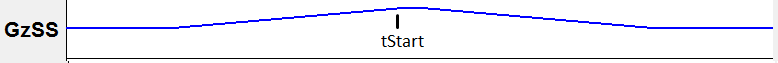
\includegraphics[width=1\textwidth]{Pictures/GzAreaTrapezoid2.eps}
	\caption{GzAreaTrapezoid2 Waveform}
	\label{fig:GzAreaTrapezoid2}
\end{figure}

\subsubsection{GzCartesian}

A GzSS macro that creates a Cartesian phase encoding gradient pulse (Figure \ref{fig:GzCartesian}) along the slice direction. This macro contains attributes including:

\begin{itemize}
	\item t1Start (s) : The phase encoding gradient pulse starting time
	\item t1End (s) : The phase encoding gradient pulse ending time
	\item t2Start (s) : The rephasing gradient pulse starting time
	\item t2End (s) : The rephasing gradient pulse ending time
	\item tRamp (s) : Gradient pulse ramp time, assume symmetric ramp on both side
	\item Gz1Sign : The polarity of the phase encoding gradient, set 0 for nulling
	\item Gz2Sign : The polarity of the rephasing gradient, set 0 for nulling
	\item Switch : The flag for turning on and off gradient pulse in the sequence line
	\item Duplicates : The number of the gradient pulse duplicates, used for creating multiple gradient pulses with the same shape
	\item DupSpacing : The time spacing between gradient pulse duplicates
	\item Notes : The notes of the gradient pulse 
\end{itemize}

Notice that the phase encoding gradient and the rephasing gradient have the same area that is automatically calculated based on the imaging parameters in the main control console.

\begin{figure}[htbp]
	\centering
		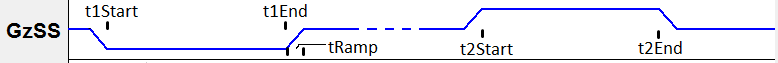
\includegraphics[width=1\textwidth]{Pictures/GzCartesian.eps}
	\caption{GzCartesian Waveform}
	\label{fig:GzCartesian}
\end{figure}

\subsubsection{GzUser}

If the user has the gradient pulse data saved in a MAT file, the user can easily import the gradient file into MRiLab by using `GzUser' macro. The gradient pulse MAT file needs to contain two matrices including `GTime' (i.e. gradient time points) and `GAmp' (i.e. gradient amplitude). Both matrices must have the same size of m-by-n, where m is the number of TR sections and n is the number of gradient waveform points. In typical MR sequence, the entire sequence is composed of multiple TR sections. The $i$th TR section uses the $i$th gradient pulse stored in the $i$th row of these two matrices. If the number of row is less than the number of TR sections, the last gradient pulse will be used for all the remaining TR sections. The `GzUser' macro contains attributes including:

\begin{itemize}
	\item GzFile : The path to the file that stores the gradient pulse data, quoted using single quotes
	\item Switch : The flag for turning on and off gradient pulse in the sequence line
	\item Duplicates : The number of the gradient pulse duplicates, used for creating multiple gradient pulses with the same shape
	\item DupSpacing : The time spacing between gradient pulse duplicates
	\item Notes : The notes of the gradient pulse 
\end{itemize}


\subsection{GyPE Macro Library}

A GyPE macro is a predefined module for a gradient pulse on the GyPE sequence line. MRiLab GyPE macro library is a collection of GyPE macros covering different gradient pulse types for performing phase encoding. Notice that by default the area under the gradient ramp is ignored. This section will give an introduction to each of the GyPE macros provided in MRiLab.

\subsubsection{GyTrapezoid}

Similar to GzTrapezoid (Figure \ref{fig:GzTrapezoid}), GyTrapezoid creates a trapezoid gradient pulse on GyPE sequence line. This macro contains attributes including:

\begin{itemize}
	\item tStart (s) : The trapezoid gradient pulse starting time
	\item tEnd (s) : The trapezoid gradient pulse ending time
	\item tRamp (s) : The trapezoid pulse ramp time, assume symmetric ramp on both side
	\item sRamp : The sample points on the ramp, use the value of 2 for ignoring the area under the ramp, use above 2 for counting the ramp area
	\item GyAmp (T) : The amplitude of the gradient
	\item Switch : The flag for turning on and off gradient pulse in the sequence line
	\item Duplicates : The number of the gradient pulse duplicates, used for creating multiple gradient pulses with the same shape
	\item DupSpacing : The time spacing between gradient pulse duplicates
	\item Notes : The notes of the gradient pulse 
\end{itemize}


\subsubsection{GyAreaTrapezoid}

Similar to GzAreaTrapezoid (Figure \ref{fig:GzAreaTrapezoid}), GyAreaTrapezoid creates a trapezoid gradient pulse of specified area on GyPE sequence line. This macro contains attributes including:

\begin{itemize}
	\item tStart (s) : The trapezoid gradient pulse starting time
	\item tEnd (s) : The trapezoid gradient pulse ending time
	\item Area (1/m) : The area under this gradient pulse
	\item Switch : The flag for turning on and off gradient pulse in the sequence line
	\item Duplicates : The number of the gradient pulse duplicates, used for creating multiple gradient pulses with the same shape
	\item DupSpacing : The time spacing between gradient pulse duplicates
	\item Notes : The notes of the gradient pulse 
\end{itemize}


\subsubsection{GyAreaTrapezoid2}

Similar to GzAreaTrapezoid2 (Figure \ref{fig:GzAreaTrapezoid2}), GyAreaTrapezoid2 creates a trapezoid gradient pulse of specified area with highest system performance on GyPE sequence line. This macro creates a gradient pulse with nearly shortest pulse width for the given system hardware constraint. This macro contains attributes including:

\begin{itemize}
	\item tStart (s) : The trapezoid gradient pulse starting time
	\item Area (1/m) : The area under this gradient pulse
	\item Switch : The flag for turning on and off gradient pulse in the sequence line
	\item Duplicates : The number of the gradient pulse duplicates, used for creating multiple gradient pulses with the same shape
	\item DupSpacing : The time spacing between gradient pulse duplicates
	\item Notes : The notes of the gradient pulse 
\end{itemize}


\subsubsection{GyCartesian}

Similar to GzCartesian (Figure \ref{fig:GzCartesian}), GyCartesian creates a Cartesian phase encoding gradient pulse on GyPE sequence line. This macro contains attributes including:

\begin{itemize}
	\item t1Start (s) : The phase encoding gradient pulse starting time
	\item t1End (s) : The phase encoding gradient pulse ending time
	\item t2Start (s) : The rephasing gradient pulse starting time
	\item t2End (s) : The rephasing gradient pulse ending time
	\item tRamp (s) : Gradient pulse ramp time, assume symmetric ramp on both side
	\item Gy1Sign : The polarity of the phase encoding gradient, set 0 for nulling
	\item Gy2Sign : The polarity of the rephasing gradient, set 0 for nulling
	\item Switch : The flag for turning on and off gradient pulse in the sequence line
	\item Duplicates : The number of the gradient pulse duplicates, used for creating multiple gradient pulses with the same shape
	\item DupSpacing : The time spacing between gradient pulse duplicates
	\item Notes : The notes of the gradient pulse 
\end{itemize}

Notice that the phase encoding gradient and the rephasing gradient have the same area that is automatically calculated based on the imaging parameters in the main control console.


\subsubsection{GyRadial}

A GyPE macro that creates a phase encoding gradient pulse for radial K-Space trajectory (Figure \ref{fig:GyRadial}) on GyPE sequence line. This macro contains attributes including:

\begin{itemize}
	\item t1Start (s) : The prephasing gradient pulse starting time
	\item t2Middle (s) : The phase encoding gradient pulse middle time
	\item t3Start (s) : The rephasing gradient pulse starting time
	\item tRamp (s) : Gradient pulse ramp time, assume symmetric ramp on both side
	\item Gy1Sign : The polarity of the prephasing gradient, set 0 for nulling
	\item Gy2Sign : The polarity of the phase encoding gradient, set 0 for nulling
  \item Gy3Sign : The polarity of the rephasing gradient, set 0 for nulling
	\item Switch : The flag for turning on and off gradient pulse in the sequence line
	\item Notes : The notes of the gradient pulse 
\end{itemize}

Notice that both the prephasing gradient and rephasing gradient have half of the area of the phase encoding gradient that is automatically calculated based on the imaging parameters in the main control console. MRiLab requires the `Radial' special technique tab to be loaded for properly configuring the `GyRadial', `GxRadial' and `ADCRadial' macro. The user can set t2Middle value as `VCtl.TE' to acquire the echo signal.

\begin{figure}[htbp]
	\centering
		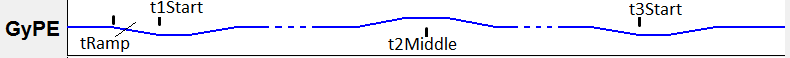
\includegraphics[width=1\textwidth]{Pictures/GyRadial.eps}
	\caption{GyRadial Waveform}
	\label{fig:GyRadial}
\end{figure}

\subsubsection{GySpiral}

A GyPE macro that creates a phase encoding gradient pulse for spiral K-Space trajectory (Figure \ref{fig:GySpiral}) on GyPE sequence line. This macro contains attributes including:

\begin{itemize}
	\item tStart (s) : The phase encoding gradient pulse starting time
	\item dt (s) : The time interval of gradient pulse sample points
	\item Switch : The flag for turning on and off gradient pulse in the sequence line
	\item Notes : The notes of the gradient pulse 
\end{itemize}

Notice that the area of the phase encoding gradient is automatically calculated based on the imaging parameters in the main control console. MRiLab requires the `Spiral' special technique tab to be loaded for properly configuring the `GySpiral', `GxSpiral' and `ADCSpiral' macro. The user can set tStart value as `VCtl.TE' to acquire the echo signal.

\begin{figure}[htbp]
	\centering
		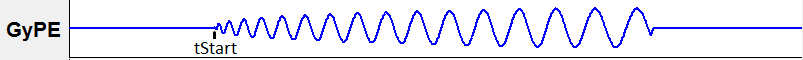
\includegraphics[width=1\textwidth]{Pictures/GySpiral.eps}
	\caption{GySpiral Waveform}
	\label{fig:GySpiral}
\end{figure}


\subsubsection{GyFSE}

A GyPE macro that creates a FSE phase encoding gradient pulse train (Figure \ref{fig:GyFSE}) on GyPE sequence line. This macro contains attributes including:

\begin{itemize}
	\item tMiddle (s) : The middle time of the gradient pulse train
	\item tOffset (s) : The time offset of the gradient pulse
	\item tGy1 (s) : The duration of the phase encoding gradient
	\item tGy2 (s) : The duration of the rephasing gradient
	\item Gy1Sign : The polarity of the phase encoding gradient, set 0 for nulling
	\item Gy2Sign : The polarity of the rephasing gradient, set 0 for nulling
	\item Switch : The flag for turning on and off gradient pulse in the sequence line
	\item Notes : The notes of the gradient pulse 
\end{itemize}

Notice that the phase encoding gradient and the rephasing gradient have the same area that is automatically calculated based on the imaging parameters in the main control console. MRiLab requires the `FSE' special technique tab to be loaded for properly configuring the `GyFSE', `GxFSE' and `ADCFSE' macro. To satisfy Carr Purcell Meiboom Gill (CPMG) condition and acquire echo signal at the center between two consecutive refocusing RF pulse, the effective TE value must equal (floor(FSE\_ETL/2)+1)*FSE\_ESP. The user can set tMiddle value as `VCtl.TE' to acquire the echo signal, where the `VCtl.TE' becomes the effective TE value.

\begin{figure}[htbp]
	\centering
		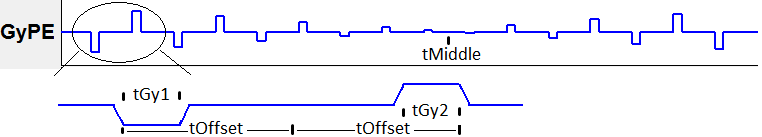
\includegraphics[width=1\textwidth]{Pictures/GyFSE.eps}
	\caption{GyFSE Waveform}
	\label{fig:GyFSE}
\end{figure}

\subsubsection{GyEPI}

A GyPE macro that creates an EPI phase encoding gradient pulse train (Figure \ref{fig:GyEPI}) on GyPE sequence line. This macro contains attributes including:

\begin{itemize}
	\item t2Middle (s) : The middle time of the blip gradient pulse train
	\item t1Start (s) : The prephasing gradient starting time
	\item Gy1Sign : The polarity of the prephasing gradient, set 0 for nulling
	\item Gy2Sign : The polarity of the blip gradient train, set 0 for nulling
	\item Switch : The flag for turning on and off gradient pulse in the sequence line
	\item Notes : The notes of the gradient pulse 
\end{itemize}

Notice that the area of the prephasing gradient and the blip gradient are automatically calculated based on the imaging parameters in the main control console. MRiLab requires the `EPI' special technique tab to be loaded for properly configuring the `GyEPI', `GxEPI' and `ADCEPI' macro. The user can set t2Middle value as `VCtl.TE' to acquire the echo signal, where the `VCtl.TE' becomes the effective TE value.

\begin{figure}[htbp]
	\centering
		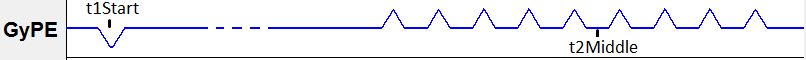
\includegraphics[width=1\textwidth]{Pictures/GyEPI.eps}
	\caption{GyEPI Waveform}
	\label{fig:GyEPI}
\end{figure}


\subsubsection{GyUser}

If the user has the gradient pulse data saved in a MAT file, the user can easily import the gradient file into MRiLab by using `GyUser' macro. The gradient pulse MAT file needs to contain two matrices including `GTime' (i.e. gradient time points) and `GAmp' (i.e. gradient amplitude). Both matrices must have the same size of m-by-n, where m is the number of TR sections and n is the number of gradient waveform points. In typical MR sequence, the entire sequence is composed of multiple TR sections. The $i$th TR section uses the $i$th gradient pulse stored in the $i$th row of these two matrices. If the number of row is less than the number of TR sections, the last gradient pulse will be used for all the remaining TR sections. The `GyUser' macro contains attributes including:

\begin{itemize}
	\item GyFile : The path to the file that stores the gradient pulse data, quoted using single quotes
	\item Switch : The flag for turning on and off gradient pulse in the sequence line
	\item Duplicates : The number of the gradient pulse duplicates, used for creating multiple gradient pulses with the same shape
	\item DupSpacing : The time spacing between gradient pulse duplicates
	\item Notes : The notes of the gradient pulse 
\end{itemize}


\subsection{GxR Macro Library}

A GxR macro is a predefined module for a gradient pulse on the GxR sequence line. MRiLab GxR macro library is a collection of GxR macros covering different gradient pulse types for performing frequency encoding. Notice that by default the area under the gradient ramp is ignored. This section will give an introduction to each of the GxR macros provided in MRiLab.

\subsubsection{GxTrapezoid}

Similar to GzTrapezoid (Figure \ref{fig:GzTrapezoid}), GxTrapezoid creates a trapezoid gradient pulse on GxR sequence line. This macro contains attributes including:

\begin{itemize}
	\item tStart (s) : The trapezoid gradient pulse starting time
	\item tEnd (s) : The trapezoid gradient pulse ending time
	\item tRamp (s) : The trapezoid pulse ramp time, assume symmetric ramp on both side
	\item sRamp : The sample points on the ramp, use the value of 2 for ignoring the area under the ramp, use above 2 for counting the ramp area
	\item GxAmp (T) : The amplitude of the gradient
	\item Switch : The flag for turning on and off gradient pulse in the sequence line
	\item Duplicates : The number of the gradient pulse duplicates, used for creating multiple gradient pulses with the same shape
	\item DupSpacing : The time spacing between gradient pulse duplicates
	\item Notes : The notes of the gradient pulse 
\end{itemize}


\subsubsection{GxAreaTrapezoid}

Similar to GzAreaTrapezoid (Figure \ref{fig:GzAreaTrapezoid}), GxAreaTrapezoid creates a trapezoid gradient pulse of specified area on GxR sequence line. This macro contains attributes including:

\begin{itemize}
	\item tStart (s) : The trapezoid gradient pulse starting time
	\item tEnd (s) : The trapezoid gradient pulse ending time
	\item Area (1/m) : The area under this gradient pulse
	\item Switch : The flag for turning on and off gradient pulse in the sequence line
	\item Duplicates : The number of the gradient pulse duplicates, used for creating multiple gradient pulses with the same shape
	\item DupSpacing : The time spacing between gradient pulse duplicates
	\item Notes : The notes of the gradient pulse 
\end{itemize}

\subsubsection{GxAreaTrapezoid2}

Similar to GzAreaTrapezoid2 (Figure \ref{fig:GzAreaTrapezoid2}), GxAreaTrapezoid2 creates a trapezoid gradient pulse of specified area with highest system performance on GxR sequence line. This macro creates a gradient pulse with nearly shortest pulse width for the given system hardware constraint. This macro contains attributes including:

\begin{itemize}
	\item tStart (s) : The trapezoid gradient pulse starting time
	\item Area (1/m) : The area under this gradient pulse
	\item Switch : The flag for turning on and off gradient pulse in the sequence line
	\item Duplicates : The number of the gradient pulse duplicates, used for creating multiple gradient pulses with the same shape
	\item DupSpacing : The time spacing between gradient pulse duplicates
	\item Notes : The notes of the gradient pulse 
\end{itemize}

\subsubsection{GxCartesian}

A GxR macro that creates a Cartesian frequency encoding gradient pulse (Figure \ref{fig:GxCartesian}) on GxR sequence line. This macro contains attributes including:

\begin{itemize}
	\item t1Start (s) : The prephasing gradient pulse starting time
	\item t2Middle (s) : The frequency encoding gradient pulse middle time
	\item t3Start (s) : The rephasing gradient pulse starting time
	\item tRamp (s) : Gradient pulse ramp time, assume symmetric ramp on both side
	\item Gx1Sign : The polarity of the prephasing gradient, set 0 for nulling
	\item Gx2Sign : The polarity of the frequency encoding gradient, set 0 for nulling
	\item Gx3Sign : The polarity of the rephasing gradient, set 0 for nulling
	\item Switch : The flag for turning on and off gradient pulse in the sequence line
	\item Duplicates : The number of the gradient pulse duplicates, used for creating multiple gradient pulses with the same shape
	\item DupSpacing : The time spacing between gradient pulse duplicates
	\item Notes : The notes of the gradient pulse 
\end{itemize}

Notice that both the prephasing gradient and rephasing gradient have half of the area of the frequency encoding gradient.

\begin{figure}[htbp]
	\centering
		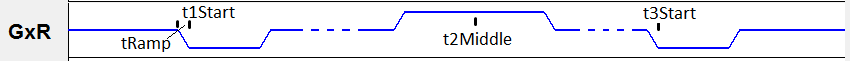
\includegraphics[width=1\textwidth]{Pictures/GxCartesian.eps}
	\caption{GxCartesian Waveform}
	\label{fig:GxCartesian}
\end{figure}		

\subsubsection{GxRadial}

Similar to GyRadial (Figure \ref{fig:GyRadial}), GxRadial creates a phase encoding gradient pulse for radial K-Space trajectory on GxR sequence line. This macro contains attributes including:

\begin{itemize}
	\item t1Start (s) : The prephasing gradient pulse starting time
	\item t2Middle (s) : The phase encoding gradient pulse middle time
	\item t3Start (s) : The rephasing gradient pulse starting time
	\item tRamp (s) : Gradient pulse ramp time, assume symmetric ramp on both side
	\item Gx1Sign : The polarity of the prephasing gradient, set 0 for nulling
	\item Gx2Sign : The polarity of the phase encoding gradient, set 0 for nulling
  \item Gx3Sign : The polarity of the rephasing gradient, set 0 for nulling
	\item Switch : The flag for turning on and off gradient pulse in the sequence line
	\item Notes : The notes of the gradient pulse 
\end{itemize}

Notice that both the prephasing gradient and rephasing gradient have half of the area of the phase encoding gradient that is automatically calculated based on the imaging parameters in the main control console. MRiLab requires the `Radial' special technique tab to be loaded for properly configuring the `GyRadial', `GxRadial' and `ADCRadial' macro. The user can set t2Middle value as `VCtl.TE' to acquire the echo signal.

\subsubsection{GxSpiral}

Similar to GySpiral (Figure \ref{fig:GySpiral}), GxSpiral creates a phase encoding gradient pulse for spiral K-Space trajectory on GxR sequence line. This macro contains attributes including:

\begin{itemize}
	\item tStart (s) : The phase encoding gradient pulse starting time
	\item dt (s) : The time interval of gradient pulse sample points
	\item Switch : The flag for turning on and off gradient pulse in the sequence line
	\item Notes : The notes of the gradient pulse 
\end{itemize}

Notice that the area of the phase encoding gradient is automatically calculated based on the imaging parameters in the main control console. MRiLab requires the `Spiral' special technique tab to be loaded for properly configuring the `GySpiral', `GxSpiral' and `ADCSpiral' macro. The user can set tStart value as `VCtl.TE' to acquire the echo signal.

\subsubsection{GxFSE}

A GxR macro that creates a FSE frequency encoding gradient pulse train (Figure \ref{fig:GxFSE}) on GxR sequence line. This macro contains attributes including:

\begin{itemize}
	\item t2Middle (s) : The middle time of the gradient pulse train
	\item t1Start (s) : The prephasing gradient starting time
	\item Gx1Sign : The polarity of the prephasing gradient, set 0 for nulling
	\item Gx2Sign : The polarity of the frequency encoding gradient train, set 0 for nulling
	\item Switch : The flag for turning on and off gradient pulse in the sequence line
	\item Notes : The notes of the gradient pulse 
\end{itemize}

Notice that the prephasing gradient has half of the area of the frequency encoding gradient that is automatically calculated based on the imaging parameters in the main control console. MRiLab requires the `FSE' special technique tab to be loaded for properly configuring the `GyFSE', `GxFSE' and `ADCFSE' macro. To satisfy CPMG condition and acquire echo signal at the center between two consecutive refocusing RF pulse, the effective TE value must equal (floor(FSE\_ETL/2)+1)*FSE\_ESP. The user can set t2Middle value as `VCtl.TE' to acquire the echo signal, where the `VCtl.TE' becomes the effective TE value.

\begin{figure}[htbp]
	\centering
		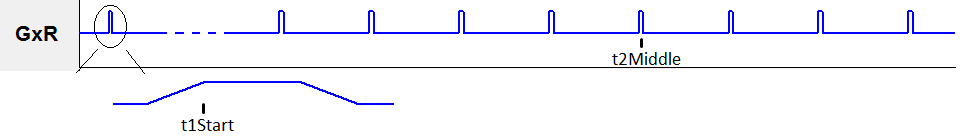
\includegraphics[width=1\textwidth]{Pictures/GxFSE.eps}
	\caption{GxFSE Waveform}
	\label{fig:GxFSE}
\end{figure}

\subsubsection{GxEPI}

A GxR macro that creates an EPI frequency encoding gradient pulse train (Figure \ref{fig:GxEPI}) on GxR sequence line. This macro contains attributes including:

\begin{itemize}
	\item t2Middle (s) : The middle time of the frequency encoding gradient pulse train
	\item t1Start (s) : The prephasing gradient starting time
	\item Gx1Sign : The polarity of the prephasing gradient, set 0 for nulling
	\item Gx2Sign : The polarity of the frequency encoding gradient train, set 0 for nulling
	\item Switch : The flag for turning on and off gradient pulse in the sequence line
	\item Notes : The notes of the gradient pulse 
\end{itemize}

Notice that the area of the prephasing gradient and the frequency encoding gradient are automatically calculated based on the imaging parameters in the main control console. MRiLab requires the `EPI' special technique tab to be loaded for properly configuring the `GyEPI', `GxEPI' and `ADCEPI' macro. The user can set t2Middle value as `VCtl.TE' to acquire the echo signal, where the `VCtl.TE' becomes the effective TE value.

\begin{figure}[htbp]
	\centering
		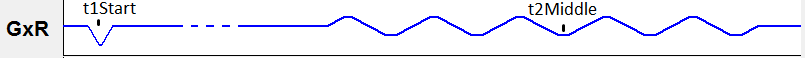
\includegraphics[width=1\textwidth]{Pictures/GxEPI.eps}
	\caption{GxEPI Waveform}
	\label{fig:GxEPI}
\end{figure}

\subsubsection{GxUser}

If the user has the gradient pulse data saved in a MAT file, the user can easily import the gradient file into MRiLab by using `GxUser' macro. The gradient pulse MAT file needs to contain two matrices including `GTime' (i.e. gradient time points) and `GAmp' (i.e. gradient amplitude). Both matrices must have the same size of m-by-n, where m is the number of TR sections and n is the number of gradient waveform points. In typical MR sequence, the entire sequence is composed of multiple TR sections. The $i$th TR section uses the $i$th gradient pulse stored in the $i$th row of these two matrices. If the number of row is less than the number of TR sections, the last gradient pulse will be used for all the remaining TR sections. The `GxUser' macro contains attributes including:

\begin{itemize}
	\item GxFile : The path to the file that stores the gradient pulse data, quoted using single quotes
	\item Switch : The flag for turning on and off gradient pulse in the sequence line
	\item Duplicates : The number of the gradient pulse duplicates, used for creating multiple gradient pulses with the same shape
	\item DupSpacing : The time spacing between gradient pulse duplicates
	\item Notes : The notes of the gradient pulse 
\end{itemize}


\subsection{ADC Macro Library}

An ADC macro is a predefined module for an ADC flag pulse on the ADC sequence line. Signal acquisition starts when ADC flag is 1 and stops when ADC flag is 0. The ADC flag pulse is sampled at certain sampling rate that is determined by the imaging parameters (default by using `BandWidth') in the main control console. MRiLab ADC macro library is a collection of ADC macros covering different pulse types for performing signal acquisition. This section will give an introduction to each of the ADC macros provided in MRiLab.

\subsubsection{ADCBlock}

An ADC macro that creates an ADC flag pulse with user defined sampling rate on ADC sequence line. This macro contains attributes including:

\begin{itemize}
	\item tStart (s) : The ADC starting time
	\item tEnd (s) : The ADC ending time
	\item sSample : The number of linear sample points when ADC flag is 1
	\item Switch : The flag for turning on and off ADC pulse in the sequence line
	\item Duplicates : The number of the ADC pulse duplicates, used for creating multiple ADC pulses with the same shape
	\item DupSpacing : The time spacing between ADC pulse duplicates
	\item Notes : The notes of the ADC pulse 
\end{itemize}

\begin{figure}[htbp]
	\centering
		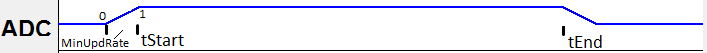
\includegraphics[width=1\textwidth]{Pictures/ADCBlock.eps}
	\caption{ADCBlock Waveform}
	\label{fig:ADCBlock}
\end{figure}


\subsubsection{ADCCartesian}

An ADC macro that creates an ADC flag pulse for Cartesian readout on ADC sequence line. This macro contains attributes including:

\begin{itemize}
	\item tMiddle (s) : The ADC middle time, typically set `VCtl.TE' for acquiring echo signal
	\item Switch : The flag for turning on and off ADC pulse in the sequence line
	\item Duplicates : The number of the ADC pulse duplicates, used for creating multiple ADC pulses with the same shape
	\item DupSpacing : The time spacing between ADC pulse duplicates
	\item Notes : The notes of the ADC pulse 
\end{itemize}

\subsubsection{ADCRadial}

An ADC macro that creates an ADC flag pulse for radial readout on ADC sequence line. This macro needs `Radial' tab to be loaded. This macro contains attributes including:

\begin{itemize}
	\item tMiddle (s) : The ADC middle time, typically set `VCtl.TE' for acquiring echo signal
	\item Switch : The flag for turning on and off ADC pulse in the sequence line
	\item Notes : The notes of the ADC pulse 
\end{itemize}

\subsubsection{ADCSpiral}

An ADC macro that creates an ADC flag pulse for spiral readout on ADC sequence line. This macro needs `Spiral' tab to be loaded. This macro contains attributes including:

\begin{itemize}
	\item tStart (s) : The ADC starting time, typically set `VCtl.TE' for acquiring echo signal
	\item Switch : The flag for turning on and off ADC pulse in the sequence line
	\item Notes : The notes of the ADC pulse 
\end{itemize}


\subsubsection{ADCFSE}

An ADC macro that creates an ADC flag pulse train for FSE readout on ADC sequence line. This macro needs `FSE' tab to be loaded. This macro contains attributes including:

\begin{itemize}
	\item tMiddle (s) : The ADC pulse train middle time, typically set `VCtl.TE' for acquiring echo signal
	\item Switch : The flag for turning on and off ADC pulse in the sequence line
	\item Notes : The notes of the ADC pulse 
\end{itemize}

\subsubsection{ADCEPI}

An ADC macro that creates an ADC flag pulse train for EPI readout on ADC sequence line. This macro needs `EPI' tab to be loaded. This macro contains attributes including:

\begin{itemize}
	\item tMiddle (s) : The ADC pulse train middle time, typically set `VCtl.TE' for acquiring echo signal
	\item Switch : The flag for turning on and off ADC pulse in the sequence line
	\item Notes : The notes of the ADC pulse 
\end{itemize}

\subsubsection{ADCUser}

If the user has the ADC pulse data saved in a MAT file, the user can easily import the ADC file into MRiLab by using `ADCUser' macro. The ADC pulse MAT file needs to contain two matrices including `GTime' (i.e. ADC time points) and `GAmp' (i.e. ADC amplitude, use 1 for signal acquisition, 0 for no signal acquisition). Both matrices must have the same size of m-by-n, where m is the number of TR sections and n is the number of ADC sample points. In typical MR sequence, the entire sequence is composed of multiple TR sections. The $i$th TR section uses the $i$th ADC pulse stored in the $i$th row of these two matrices. If the number of row is less than the number of TR sections, the last ADC pulse will be used for all the remaining TR sections. The `ADCUser' macro contains attributes including:

\begin{itemize}
	\item ADCFile : The path to the file that stores the ADC pulse data, quoted using single quotes
	\item Switch : The flag for turning on and off ADC pulse in the sequence line
	\item Duplicates : The number of the ADC pulse duplicates, used for creating multiple ADC pulses with the same shape
	\item DupSpacing : The time spacing between ADC pulse duplicates
	\item Notes : The notes of the ADC pulse 
\end{itemize}

Notice that `ADCUser' macro sets the first and last ADC sample points to 0 regardless of their original value, therefore the signal is not acquired at the first and last time points.

\subsection{Ext Macro Library} \label{subs:ExtMacroLibrary}

An Ext macro is a predefined module for an Ext flag pulse on the Ext sequence line. MRiLab specifies Ext signal for performing extended real time processes including calculating remaining scan time, manipulating K-Space location and triggering object motion etc. Ext macro library only contains `ExtBit' macro, however the `Ext' attribute in this macro triggers different processes. 

\subsubsection{ExtBit}

The `ExtBit' macro (Figure \ref{fig:ExtBit}) creates a triangle blip pulse on Ext sequence line. This macro contains attributes including:

\begin{itemize}
	\item tStart (s) : The Ext starting time
	\item Ext : The Ext flag
	\item Switch : The flag for turning on and off Ext pulse in the sequence line
	\item Duplicates : The number of the Ext pulse duplicates, used for creating multiple Ext pulses with the same shape
	\item DupSpacing : The time spacing between Ext pulse duplicates
	\item Notes : The notes of the Ext pulse 
\end{itemize}

\begin{figure}[htbp]
	\centering
		\includegraphics[width=1\textwidth]{Pictures/ExtBit.eps}
	\caption{ExtBit Waveform}
	\label{fig:ExtBit}
\end{figure}


Different Ext flags execute different extended real time processes during runtime scan. These extended processes are implemented using Plugin code in the /Plugin folder. MRiLab reserved several Ext flags for particular purposes. 

\begin{itemize}
	\item 1 : Plugin\_ResetK, reset Kx, Ky and Kz to zero
	\item 2 : Plugin\_ReverseK, reverse Kx, Ky and Kz
	\item 3 : Plugin\_LockK, buffer current K space location
	\item 4 : Plugin\_ReleaseK, set K space location to the latest buffered one, used after Plugin\_LockK
	\item 5 : Plugin\_Timer, calculate remaining scan time, display it on the main control console
	\item 6 : Plugin\_IdealSpoiler, dephase transverse magnetization of all the spins, set them to zero
	\item 7 : Plugin\_rfRef, buffer current rfPhase value and demodulate signal phase according to this value
	\item 8 : Plugin\_ExecuteMotion, trigger object motion
	\item 9 : Plugin\_RTRecon, trigger real time image reconstruction with currently stored K-Space data
\end{itemize}

\subsection{Make New Ext Plugin}

The user can define Ext flags and use Ext Plugin to create extended real time process. To make your own Ext flag and Plugin code, you should follow the following steps :

\begin{enumerate}

\item Write Ext Plugin code \\

It is strongly recommended to write your Plugin code based on a template like :

\begin{verbatim}

function Plugin_YourPluginName
%Create a Ext Plugin based on your code
global VCtl     % use VCtl structure, read only
global VVar     % use VVar structure, read only
global VObj     % use VObj structure, read and write
global VMag     % use VMag structure, read and write
global VCoi     % use VCoi structure, read and write

...
% The main code for your Ext Plugin
...

end


\end{verbatim}

As mentioned before, VCtl encapsules all the simulation setting parameters in the main control console. VVar not only encapsules the loop index variables that MRiLab uses for generating MR sequence waveform, but also contains variables for temporarily buffering instant sequence line values during runtime. \textbf{Do keep in mind, VCtl and VVar are read only, changing values inside these two structures may cause MRiLab crash.}

\begin{itemize}
	\item VVar.rfAmp (T) : A array with the size of $ TxCoilNum \times 1 $ for storing current RF amplitude
	\item VVar.rfPhase (rad) : A array with the size of $ TxCoilNum \times 1 $ for storing current RF phase
	\item VVar.rfFreq (Hz) : A array with the size of $ TxCoilNum \times 1 $ for storing current RF frequency
	\item VVar.rfCoil : The CoilID of current working coil channel, used in multiple RF transmitting
	\item VVar.rfRef (rad) : The buffered RF phase, used for demodulating signal phase at ADC
	\item VVar.GzAmp (T/m) : The current GzSS gradient amplitude
	\item VVar.GyAmp (T/m) : The current GyPE gradient amplitude
	\item VVar.GxAmp (T/m) : The current GXR gradient amplitude
	\item VVar.ADC : The current ADC flag
	\item VVar.Ext : The current Ext flag
	\item VVar.t (s) : The current time
	\item VVar.Kz (1/m) : The current Kz value
	\item VVar.Ky (1/m) : The current Ky value
	\item VVar.Kx (1/m) : The current Kx value
	\item VVar.TRCount : The current TR section index
\end{itemize}


Notice that there are three new Virtual Structures (VObj, VMag and VCoi) in this template, they store the variables about the virtual object, B0 field and coil B1 field which are accessible and editable in Plugin code. \textbf{Do keep in mind, do not change the size of the matrices inside these three structures.}

\begin{itemize}
	\item VObj.Rho : A matrix with the size of $ YDim \times XDim \times ZDim \times TypeNum $ for describing spin density
	\item VObj.T1 (s) : A matrix with the size of $ YDim \times XDim \times ZDim \times TypeNum $ for describing T1 relaxation time
	\item VObj.T2 (s) : A matrix with the size of $ YDim \times XDim \times ZDim \times TypeNum $ for describing T2 relaxation time
	\item VObj.Mx : A matrix with the size of $ YDim \times XDim \times ZDim \times SpinPerVoxel \times TypeNum $ for describing magnetization in $x$ direction
	\item VObj.My : A matrix with the size of $ YDim \times XDim \times ZDim \times SpinPerVoxel \times TypeNum $ for describing magnetization in $y$ direction
	\item VObj.Mz : A matrix with the size of $ YDim \times XDim \times ZDim \times SpinPerVoxel \times TypeNum $ for describing magnetization in $z$ direction
	\item VMag.dWRnd (rad/s) : A matrix with the size of $ YDim \times XDim \times ZDim \times SpinPerVoxel \times TypeNum $ for describing microscopic resonance frequency variation caused by T2* effect
	\item VMag.dB0 (T) : A matrix with the size of $ YDim \times XDim \times ZDim $ for describing local B0 field variation
	\item VMag.Gxgrid (m) : A matrix with the size of $ YDim \times XDim \times ZDim $ for describing spatial grid in X direction
	\item VMag.Gygrid (m) : A matrix with the size of $ YDim \times XDim \times ZDim $ for describing spatial grid in Y direction
	\item VMag.Gzgrid (m) : A matrix with the size of $ YDim \times XDim \times ZDim $ for describing spatial grid in Z direction
	\item VCoi.TxCoilmg (T) : A matrix with the size of $ YDim \times XDim \times ZDim \times TxCoilNum $ for describing the magnitude of transmitting B1+ field
	\item VCoi.TxCoilpe (rad) : A matrix with the size of $ YDim \times XDim \times ZDim \times TxCoilNum $ for describing the phase of transmitting B1+ field
	\item VCoi.RxCoilx (T) : A matrix with the size of $ YDim \times XDim \times ZDim \times RxCoilNum $ for describing the $x$ component of receiving B1- field
	\item VCoi.RxCoily (T) : A matrix with the size of $ YDim \times XDim \times ZDim \times RxCoilNum $ for describing the $y$ component of receiving B1- field
\end{itemize}

where `TxCoilNum' is the number of transmitting coil channels, `RxCoilNum' is the number of receiving coil channels.

\item Register Ext Plugin \\

The user needs to register customized Plugins before MRiLab can use it. To register Plugins and assign Ext flags to them, simply open `DoExtPlugin.m' under /Src folder.

\begin{verbatim}
function DoExtPlugin
% entry function for extended plugin based on Ext flag
global VVar

switch VVar.Ext
%% System Reserved Ext Flags (Positive)   
    case 0 % normal status
        % do nothing
    case 1 % reset K space location
        Plugin_ResetK;
    case 2 % reverse K space location
        Plugin_ReverseK;
    case 3 % lock K space location
        Plugin_LockK;
    case 4 % release K space location
        Plugin_ReleaseK;
    case 5 % calculate remaining scan time
        Plugin_Timer;
    case 6 % ideal spoiler, dephase Mxy
        Plugin_IdealSpoiler;
    case 7 % rfRef, demodulate signal phase referring to RF phase at ADC
        Plugin_rfRef;
    case 8 % trigger object motion
        Plugin_ExecuteMotion;
    case 9 % real time image recon
        Plugin_RTRecon;

%% User Defined Ext Flags (Negative)
% add user defined Ext flags here using case syntax
% e.g.    case -5
%             Plugin_XXX;

end
end
\end{verbatim}

Add one more Switch case line, assign a distinct Ext flag, then add user defined Plugin function name under the case line. It is recommended to use negative Ext flag for user defined Plugin to make differences from system reserved plugins.

\item Register to refresh GPU device memory \\

If the customized Plugin function modifies any variables in VObj, VMag or VCoi, the Plugin function needs to be registered for refreshing GPU device memory in case GPU parallel computing method is chosen. Simply open `DoGPUFetch.m' under /Src folder.

\begin{verbatim}
function DoGPUFetch
% fetch data from GPU?
% VVar.gpuFetch = 1  fetch data from GPU memory to CPU memory
% VVar.gpuFetch = 0  no GPU data fetching
global VVar

switch VVar.Ext
%% System Reserved Ext Flags (Positive)   
    case 6 % ideal spoiler, dephase Mxy
        VVar.gpuFetch = 1;
    case 8 % trigger object motion
        VVar.gpuFetch = 1;
				
				
%% User Defined Ext Flags (Negative)
% add user defined Ext flags here using case syntax
% e.g.    case -5
%             VVar.gpuFetch = 1;

end
end
\end{verbatim}

Add one more Switch case line, assign VVar.gpuFetch equal to 1. 

\end{enumerate}

\subsection{Make New Gradient Macro}

The user can make customized gradient macros and use them to create desired K-Space trajectory. To make your own gradient macro, you should follow the following steps :


\begin{enumerate}

\item Write gradient macro code \\

It is strongly recommended to write your own gradient macro code based on the closest gradient macros in the MRiLab macro library. One template is like :

\begin{verbatim}
function [GAmp,GTime]=GYourGradientMacroName(p)
%Create a gradient macro based on your code

global VCtl     % use VCtl structure, read only
global VObj     % use VObj structure, read only

% Create attribute list
Duplicates=max(1,p.Duplicates);
DupSpacing=max(0,p.DupSpacing);
...
attribute1=p.attribute1;
attribute2=p.attribute2;
attribute3=p.attribute3;
...

% The main code for your macro
...
GTime = ...;
GAmp = ...;
...

% Avoid baseline offset
GAmp(1)=0;
GAmp(end)=0;

% Create Duplicates
if Duplicates~=1 & DupSpacing ~=0
    GAmp=repmat(GAmp,[1 Duplicates]);
    TimeOffset = repmat(0:DupSpacing:(Duplicates-1)*DupSpacing, ...
                       [length(GTime) 1]);
    GTime=repmat(GTime,[1 Duplicates]) + (TimeOffset(:))';
end
end
\end{verbatim}

\item Register gradient macro \\

The gradient macro file can be located anywhere in the computer as long as the file is included in Matlab searching path, however it is recommended to save the the file under corresponding gradient folder under /SeqElem folder for consistent file organization. The customized gradient macro needs to be registered in the macro library before using. To register the macro, open file `SeqElem.xml' under /SeqElem, then add one entry under gradient category with the proper attribute list. One example could be

\begin{verbatim}
<GzGradientMacroName  
				Switch="$1'on','off'" 
				DupSpacing="0" 
				Duplicates="1" 
				Notes="A new Gz gradient macro" 
				attribute1="$1'on','off'" 
				attribute2="0" 
				attribute3="0" />
				
\end{verbatim}

Notice that in the above example, the first 3 attributes are required for MRiLab, The remaining attributes are optional based on user's choice.

\end{enumerate}

Once the gradient macro is coded and registered to the library, the user can use this customized gradient macro just like those default gradient macros in the library.

\subsection{Make New MR Sequence}

To design a sequence in the MR Sequence Design interface, it is recommended to load the sequence into the main control console first and then click toolbar icon to activate the MR Sequence Design interface. This is mainly because the associated imaging parameters that are necessary for configuring current sequence will also be loaded during the sequence loading process. However, if the interface has already been activated, the user can also use the sequence loading function to load another sequence with current imaging parameters. To load a sequence, click `Load' menu then click `Load Sequence File', choose a sequence XML file.\\

The user can create a new MR sequence in the MR Sequence Design interface. To create a new sequence, click `New' then click `Create Sequence File'. A sequence creation window (Figure \ref{fig:NewPSD}) will show up and ask for new sequence name and notes. To follow MRiLab naming convention, the user is recommended to use `PSD\_' followed by a legal name string that is distinct to the existing sequences in MRiLab. Then click `OK' to select a path for storing the sequence XML file. It's strongly recommended to put the sequence under the MRiLab sequence root folder /PSD according to the sequence type so that the sequence is visible to MRiLab. Finally, MRiLab will create a new sequence XML file based on the content of `PSD\_GRE3D'.

\begin{figure}[htbp]
	\centering
		\includegraphics[width=0.3\textwidth]{Pictures/NewPSD.eps}
	\caption{The Sequence Creation Window}
	\label{fig:NewPSD}
\end{figure}


\subsection{Make New Virtual Object}

To design and optimize MR sequence, the user may need virtual objects with specific geometry and properties according to their experiment purpose. Although MRiLab provides a few phantoms with tissue properties mimicking several human tissue types, the user may still need to define customized virtual object. To make your own virtual object, you should follow the following steps :

\begin{enumerate}

\item Make Regular Virtual Object \\

Create a Matlab structure `VObj'. `VObj' must contains variables including:

\begin{itemize}
	\item Gyro (rad/s/T) : The gyromagnetic ratio of the spin
	\item ChemShift (Hz/T) : A array with the size of $1 \times TypeNum $ for describing the chemical shift of the spins
	\item XDim : The number of voxels in X direction
	\item YDim : The number of voxels in Y direction
	\item ZDim : The number of voxels in Z direction
	\item XDimRes (m) : The voxel size in X direction
	\item YDimRes (m) : The voxel size in Y direction
	\item ZDimRes (m) : The voxel size in Z direction
	\item Type : A string for describing the type of the spin
	\item TypeNum : The number of spin species
	\item Rho : A matrix with the size of $ YDim \times XDim \times ZDim \times TypeNum $ for describing spin density
	\item T1 (s) : A matrix with the size of $ YDim \times XDim \times ZDim \times TypeNum $ for describing T1 relaxation time
	\item T2 (s) : A matrix with the size of $ YDim \times XDim \times ZDim \times TypeNum $ for describing T2 relaxation time
	\item T2Star (s) : A matrix with the size of $ YDim \times XDim \times ZDim \times TypeNum $ for describing T2* relaxation time
\end{itemize}

Then save the `VObj' structure as a MAT file.

\item Make Virtual Object with Magnetization Transfer (MT) Properties\\

The current MRiLab version only supports two-pool MT model \cite{Yarnykh2002} with GPU acceleration. The `VObj' must have the structure like:

\begin{itemize}
	\item Gyro (rad/s/T) : The gyromagnetic ratio of the spin
	\item ChemShift (Hz/T) : A array with the size of $1 \times 2 $ for describing the chemical shift of the spins, free pool first, bound pool second
	\item XDim : The number of voxels in X direction
	\item YDim : The number of voxels in Y direction
	\item ZDim : The number of voxels in Z direction
	\item XDimRes (m) : The voxel size in X direction
	\item YDimRes (m) : The voxel size in Y direction
	\item ZDimRes (m) : The voxel size in Z direction
	\item Type : A string for describing the type of the spin
	\item TypeNum : 2
	\item Rho : A matrix with the size of $ YDim \times XDim \times ZDim \times 2 $ for describing spin density, $Rho_{f}$ (free pool) first, $Rho_{b}$ (bound pool) second
	\item T1 (s) : A matrix with the size of $ YDim \times XDim \times ZDim \times 2 $ for describing T1 relaxation time, free pool first, bound pool second
	\item T2 (s) : A matrix with the size of $ YDim \times XDim \times ZDim \times 2 $ for describing T2 relaxation time, free pool first, bound pool second
	\item T2Star (s) : A matrix with the size of $ YDim \times XDim \times ZDim \times 2 $ for describing T2* relaxation time, free pool first, bound pool second
	\item K (1/s) : A matrix with the size of $ YDim \times XDim \times ZDim \times 4 $ for describing MT cross-relaxation rate, the $K_{fb}$ (free pool to bound pool) and the $K_{bf}$ (bound pool to free pool) is the second and third volume at the last dimension, respectively. The cross-relaxation rate to itself for any pool (i.e. $K_{ff}$ and $K_{bb}$) is assumed to be zero.
\end{itemize}

Notice that the two-pool MT model needs to satisfy chemical equilibrium described as $Rho_{f} \times K_{fb} = Rho_{b} \times K_{bf}$. After making VObj, then save the `VObj' structure as a MAT file. In MRiLab, the Bloch-equation solving kernel is only executed when the value of any sequence line needs to be updated. The time point at which this updating is happening is referred to as execution point. To accurately model MT exchange during scan, the user needs to create execution points on the entire RF sequence line. A typical method is to insert a long RF pulse with zero amplitude at the empty portion of the RF sequence line. The interested users are referred to PSD\_SPGR3DMT for more information.

\item Make Virtual Object with Multiple pool spin Exchange (ME) Properties\\

The current MRiLab version supports multiple spin exchange model up to any number of spin pools with GPU acceleration. The `VObj' must have the structure like:

\begin{itemize}
	\item Gyro (rad/s/T) : The gyromagnetic ratio of the spin
	\item ChemShift (Hz/T) : A array with the size of $1 \times Pool Number $ for describing the chemical shift of the spins
	\item XDim : The number of voxels in X direction
	\item YDim : The number of voxels in Y direction
	\item ZDim : The number of voxels in Z direction
	\item XDimRes (m) : The voxel size in X direction
	\item YDimRes (m) : The voxel size in Y direction
	\item ZDimRes (m) : The voxel size in Z direction
	\item Type : A string for describing the type of the spin
	\item TypeNum : Pool Number
	\item Rho : A matrix with the size of $ YDim \times XDim \times ZDim \times TypeNum $ for describing spin density
	\item T1 (s) : A matrix with the size of $ YDim \times XDim \times ZDim \times TypeNum $ for describing T1 relaxation time
	\item T2 (s) : A matrix with the size of $ YDim \times XDim \times ZDim \times TypeNum $ for describing T2 relaxation time
	\item T2Star (s) : A matrix with the size of $ YDim \times XDim \times ZDim \times TypeNum $ for describing T2* relaxation time
	\item K (1/s) : A matrix with the size of $ YDim \times XDim \times ZDim \times TypeNum^2 $ for describing ME exchange rate. To explain the order of the exchange rate at the last dimension, for example, given there are three pools, the exchange rate is ordered in the fashion as the first pool to itself $K_{11}$, the second pool $K_{12}$, the third pool $K_{13}$, followed by the second pool to the first pool $K_{21}$, itself $K_{22}$, the third pool $K_{23}$, followed by the third pool to the first pool $K_{31}$, the second pool $K_{32}$ and itself $K_{33}$. The exchange rate to itself for any pool is assumed to be zero.
\end{itemize}

Notice that the multiple-pool ME model also needs to satisfy chemical equilibrium analogous to that of MT model. After making VObj, then save the `VObj' structure as a MAT file. To accurately model ME exchange during scan, the user also needs to create execution points on the entire RF sequence line. A typical method is to insert a long RF pulse with zero amplitude at the empty portion of the RF sequence line. The interested users are referred to PSD\_SPGR3DME for more information.

\end{enumerate}

\section{Coil B1 Design}

The Coil B1 Design toolbox can be activated by pressing `Coil Design Panel' toolbar icon located at the top of the main simulation console. Depending on the coil mode (i.e. `Tx' or `Rx') highlighted on the `Coil Selection' panel, the loaded coil will show in the Coil B1 Design interface.

\begin{figure}[htbp]
	\centering
		\includegraphics[width=0.08\textwidth]{Pictures/CoilDesignPanelIcon.eps}
	\caption{Coil Design Panel Toolbar Icon}
	\label{fig:CoilDesignPanelIcon}
\end{figure}

\subsection{Coil Design GUI}

\begin{figure}[htbp]
	\centering
		\includegraphics[width=1\textwidth]{Pictures/CoilDesignGUI.eps}
	\caption{Coil B1 Design Panel. An eight channel coil is shown.}
	\label{fig:CoilDesignGUI}
\end{figure}

Figure \ref{fig:CoilDesignGUI} demonstrates an overview of the Coil B1 Design interface. This interface consists of 

\begin{enumerate}
	\item Coil Element Macro Library \\
	
The Coil Element Macro Library contains coil element macros for constructing coil structure in MRiLab. The user needs to click the `CoilElem' root to unfold subsequent macros.

	\item Coil Structure \\
	
In MRiLab, a coil structure consists of arbitrary number of coil elements that are combined to create desired B1 field. The user can construct desired B1 field by changing the content within the coil structure. To add a macro into the coil structure, the user needs to click one macro in the macro library, then click on the coil structure root (i.e. MRiLabCoil) to which this macro is inserted, then click `+' macro operation button. To delete a macro from the coil structure, the user needs to click the unwanted macro, then click `-' macro operation button. To duplicate an existing macro, the user needs to first click the source macro, then click `C' macro operation button for copying, click on the coil structure root, then click `P' macro operation button for pasting. MRiLab doesn't allow empty coil structure.
	
	
	\item Coil Element Attribute \\
	
Upon clicking on the coil element macro within the coil structure, the corresponding macro attributes will be shown at the coil element attribute panel down below the coil structure. The user can edit those attributes to modify the coil element so as to generate different B1 field. To make any modification effective, the user must press `Update' button to update the coil file. Pressing `Execute' button will update and redraw the B1 field map on this interface.
	
	\item Coil B1 Field \\

The coil configuration and B1 field (T) generated based on the coil structure is displayed on the `Coil Sensitivity' panel on the right side of this interface.
	
	\item Coil Simulation Control \\

The `Display' and `Grid' tab on the `Coil Simulation' panel contains parameters for controlling B1 field display.

\begin{itemize}
	\item Colormap : The colormap for the B1 field, includes `Jet', `Gray' and `Hot'
	\item CLimDown (T) : The lower bound of color limits
	\item CLimUp (T) : The upper bound of color limits
	\item CoilDisplay : The flag for turning on and off coil display
	\item CoilShow : The flag for choosing active coil for B1 field display
	\item Mode : The B1 field display mode, includes `Magnitude', `Phase', `Real' and `Imaginary'
	\item Plane : The flag for activating B1 field slicing plane, includes `XY', `XZ' and `YZ'
	\item XDimRes (m) : The display spatial resolution in X direction
	\item YDimRes (m) : The display spatial resolution in Y direction
	\item ZDimRes (m) : The display spatial resolution in Z direction
\end{itemize}	

\end{enumerate}

MRiLab provides a group of B1 field display button (Figure \ref{fig:B1DisplayButton}) to help inspect the B1 field details.

\begin{figure}[htbp]
	\centering
		\includegraphics[width=0.2\textwidth]{Pictures/B1DisplayButton.eps}
	\caption{The B1 Field Display Button.}
	\label{fig:B1DisplayButton}
\end{figure}

The B1 field display button group consists of:

\begin{itemize}
	\item $\wedge$ : Undock B1 field on active B1 slicing plane (Figure \ref{fig:B1Field})
	\item S+ : Move active B1 slicing plane forwards
	\item S- : Move active B1 slicing plane backwards
\end{itemize}


\begin{figure}[htbp]
	\centering
		\includegraphics[width=0.6\textwidth]{Pictures/B1Field.eps}
	\caption{An Example of B1 Field on XY Plane.}
	\label{fig:B1Field}
\end{figure}


\subsection{Coil Element Macro Library}

A coil element macro is a predefined module for creating a coil element that generates B1 field in three dimensional space. MRiLab coil element macro library is a collection of coil element macros covering simple coil geometries. This section will give an introduction to each of the coil element macro provided in MRiLab.

\subsubsection{CoilCircle}

A coil element macro that creates a Biot-Savart coil circle. This macro contains attributes including:

\begin{itemize}
	\item Azimuth (rad) : The azimuth angle of the circle plane
	\item Elevation (rad) : The elevation angle of the circle plane
	\item Radius (m) : The coil circle radius
	\item PosZ (m) : The Z position of coil circle center
  \item PosY (m) : The Y position of coil circle center
	\item PosX (m) : The X position of coil circle center
	\item CurrentDir : The current direction in the coil circle, 1 for clockwise, -1 for counterclockwise
	\item Scale : The scale factor for the B1 field amplitude
	\item Segment : The number of line segments for approximating circle, MRiLab requires the same `Segment' for each coil circle
	\item CoilID : The assigned coil ID, each coil element must have distinct ID
\end{itemize}

\subsubsection{CoilUser}

If the user has the B1 field data saved in a MAT file, the user can easily import the B1 field into MRiLab coil design interface by using `CoilUser' macro. The B1 field MAT file needs to contain two matrices including `B1x' (i.e. $x$ component of B1 field) and `B1y' (i.e. $y$ component of B1 field). Both of the two matrices must have the same size. The `CoilUser' macro contains attributes including:

\begin{itemize}
	\item B1File : The path to the file that stores the B1 field data, quoted using single quotes
	\item Interp : The interpolation method, includes `linear', `nearest' and `cubic'
	\item PosZ (m) : The Z position of coil center (needed for coil display purpose)
  \item PosY (m) : The Y position of coil center (needed for coil display purpose)
	\item PosX (m) : The X position of coil center (needed for coil display purpose)
	\item CoilID : The assigned coil ID, each coil element must have a distinct ID
\end{itemize}

\subsection{Make New Coil}

The user can also use the coil loading function to load another coil. To load a coil, click `Load' menu then click `Load Coil File', choose a coil XML file. After the coil is loaded, press `Execute' to display field.\\

The user can create a new coil configuration in the Coil Design interface. To create a new coil, click `New' then click `Create Coil File'. A coil creation window (Figure \ref{fig:NewCoil}) will show up and ask for new coil name and notes. To follow MRiLab naming convention, the user is recommended to use `Coil\_' followed by the number of coil elements and applied anatomy (e.g. Coil\_16ChChest), make sure that the new coil name is distinct to the existing coil names in MRiLab. Then click `OK' to select a path for storing the coil XML file. It's strongly recommended to put the coil under the MRiLab coil root folder /Coil according to the coil type so that the coil is visible to MRiLab. Finally, MRiLab will create a new coil XML file based on the content of `Coil\_1ChHead'.

\begin{figure}[htbp]
	\centering
		\includegraphics[width=0.3\textwidth]{Pictures/NewCoil.eps}
	\caption{The Coil Creation Window}
	\label{fig:NewCoil}
\end{figure}


\section{Magnet dB0 Design}

The Magnet dB0 Design toolbox can be activated by pressing `Magnet Design Panel' toolbar icon located at the top of the main simulation console. The loaded magnet will show in the Magnet dB0 Design interface.

\begin{figure}[htbp]
	\centering
		\includegraphics[width=0.08\textwidth]{Pictures/MagnetDesignPanelIcon.eps}
	\caption{Magnet Design Panel Toolbar Icon}
	\label{fig:MagnetDesignPanelIcon}
\end{figure}

\subsection{Magnet Design GUI}

\begin{figure}[htbp]
	\centering
		\includegraphics[width=1\textwidth]{Pictures/MagnetDesignGUI.eps}
	\caption{Magnet dB0 Design Panel}
	\label{fig:MagnetDesignGUI}
\end{figure}

Figure \ref{fig:MagnetDesignGUI} demonstrates an overview of the Magnet dB0 Design interface. This interface consists of 

\begin{enumerate}
	\item Magnet Element Macro Library \\
	
The Magnet Element Macro Library contains magnet element macros for constructing magnet structure in MRiLab. The user needs to click the `MagElem' root to unfold subsequent macros.
	
	\item Magnet Structure \\
	
In MRiLab, a magnet structure consists of arbitrary number of magnet elements that are combined to create desired dB0 field. The user can construct desired dB0 field by changing the content within the magnet structure. To add a macro into the magnet structure, the user needs to click one macro in the macro library, then click on the magnet structure root (i.e. MRiLabMag) to which this macro is inserted, then click `+' macro operation button. To delete a macro from the magnet structure, the user needs to click the unwanted macro, then click `-' macro operation button. To duplicate an existing macro, the user needs to first click the source macro, then click `C' macro operation button for copying, click on the magnet structure root, then click `P' macro operation button for pasting. MRiLab doesn't allow empty magnet structure.
	
	\item Magnet Element Attribute \\
	
Upon clicking on the magnet element macro within the magnet structure, the corresponding macro attributes will be shown at the magnet element attribute panel down below the magnet structure. The user can edit those attributes to modify the magnet element so as to generate different dB0 field. To make any modification effective, the user must press `Update' button to update the magnet file. Pressing `Execute' button will update and redraw the dB0 field map on this interface.	
	
	\item Magnet Field \\
	
The dB0 field (T) generated based on the magnet structure is displayed on the `Magnet Field' panel on the right side of this interface.
	
	\item Magnet Simulation Control \\
	
The `Display' and `Grid' tab on the `Magnet Simulation' panel contains parameters for controlling dB0 field display.

\begin{itemize}
	\item Colormap : The colormap for the dB0 field, includes `Jet', `Gray' and `Hot'
	\item Plane : The flag for activating dB0 field slicing plane, includes `XY', `XZ' and `YZ'
	\item XDimRes (m) : The display spatial resolution in X direction
	\item YDimRes (m) : The display spatial resolution in Y direction
	\item ZDimRes (m) : The display spatial resolution in Z direction
\end{itemize}	

\end{enumerate}

MRiLab provides a group of dB0 field display button to help inspect the dB0 field details. The dB0 field display button group consists of:

\begin{itemize}
	\item S+ : Move active dB0 field slicing plane forwards
	\item S- : Move active dB0 field slicing plane backwards
\end{itemize}

\subsection{Magnet Element Macro Library}

A magnet element macro is a predefined module for creating a magnet element that generates dB0 field in three dimensional space. MRiLab magnet element macro library is a collection of magnet element macros. This section will give an introduction to each of the magnet element macro provided in MRiLab.

\subsubsection{MagLinear}

A magnet element macro that creates a linear dB0 field. This macro contains attributes including:

\begin{itemize}
	\item GradZ (T/m) : The linear gradient of dB0 field in Z direction
  \item GradY (T/m) : The linear gradient of dB0 field in Y direction
	\item GradX (T/m) : The linear gradient of dB0 field in X direction
	\item Scale : The scale factor for the dB0 field
\end{itemize}

\subsubsection{MagGaussian}

A magnet element macro that creates a 3D Gaussian dB0 field. This macro contains attributes including:

\begin{itemize}
	\item PosZ (m) : The Z position of the center
  \item PosY (m) : The Y position of the center
	\item PosX (m) : The X position of the center
	\item DeltaZ (m) : The width of Gaussian function in Z direction
  \item DeltaY (m) : The width of Gaussian function in Y direction
	\item DeltaX (m) : The width of Gaussian function in X direction
	\item Scale : The scale factor for the dB0 field
\end{itemize}


\subsubsection{MagSymbolic}

A magnet element macro that creates a dB0 field based on symbolic equation. This macro contains attributes including:

\begin{itemize}
	\item Equation : An dB0 field equation
\end{itemize}

The symbolic equation could be any legal Matlab equation using variables `X', `Y' and `Z'. For example, `X+Y', `2*X.*Y' and `2*sin(X)' etc. Notice that use element operations for variables in the equation. The user needs to fill the equation between a pair of single quotes.

\subsubsection{MagUser}

If the user has the dB0 field data saved in a MAT file, the user can easily import the dB0 field into MRiLab magnet design interface by using `MagUser' macro. The dB0 field MAT file needs to contain one matrix `dB0'. The `MagUser' macro contains attributes including:

\begin{itemize}
	\item MagFile : The path to the file that stores the dB0 field data, quoted using single quotes
	\item Interp : The interpolation method, includes `linear', `nearest' and `cubic'
\end{itemize}

\subsection{Make New Magnet}

The user can also use the magnet loading function to load another magnet. To load a magnet, click `Load' menu then click `Load Magnet File', choose a magnet XML file.\\

The user can create a new magnet in the Magnet Design interface. To create a new magnet, click `New' then click `Create Magnet File'. A magnet creation window will show up and ask for new magnet name and notes. To follow MRiLab naming convention, the user is recommended to use `Mag\_' followed by a legal string and applied anatomy (e.g. Mag\_CustomHead), make sure that the new magnet name is distinct to the remaining magnet names in MRiLab. Then click `OK' to select a path for storing the magnet XML file. It's strongly recommended to put the magnet under the MRiLab magnet root folder /Mag according to the magnet type so that the magnet is visible to MRiLab. Finally, MRiLab will create a new magnet XML file based on the content of `Mag\_LinearHead'.

\section{Gradient Design}

The Gradient Design toolbox can be activated by pressing `Gradient Design Panel' toolbar icon located at the top of the main simulation console. The loaded gradient will show in the Gradient Design interface.

\begin{figure}[htbp]
	\centering
		\includegraphics[width=0.08\textwidth]{Pictures/GradientDesignPanelIcon.eps}
	\caption{Gradient Design Panel Toolbar Icon}
	\label{fig:GradientDesignPanelIcon}
\end{figure}

\subsection{Gradient Design GUI}

\begin{figure}[htbp]
	\centering
		\includegraphics[width=1\textwidth]{Pictures/GradientDesignGUI.eps}
	\caption{Gradient Design Panel}
	\label{fig:GradientDesignGUI}
\end{figure}

Figure \ref{fig:GradientDesignGUI} demonstrates an overview of the Gradient Design interface. This interface consists of 


\begin{enumerate}
	\item Gradient Element Macro Library \\
	
The Gradient Element Macro Library contains gradient element macros for constructing gradient structure in MRiLab. The user needs to click the `GradElem' root to unfold subsequent macros.

	\item Gradient Structure \\
	
In MRiLab, a gradient structure consists of three gradient elements that are combined to create gradient field for GzSS, GyPE and GxR. The user can construct desired gradient field by changing the content within the gradient structure. To add a macro into the gradient structure, the user needs to click one macro in the macro library, then click on the gradient structure root (i.e. MRiLabGrad) to which this macro is inserted, then click `+' macro operation button. To delete a macro from the gradient structure, the user needs to click the unwanted macro, then click `-' macro operation button. To duplicate an existing macro, the user needs to first click the source macro, then click `C' macro operation button for copying, click on the gradient structure root, then click `P' macro operation button for pasting. MRiLab doesn't allow empty gradient structure, and also requires each of the three gradient sequence lines must have an individual gradient field.	
	
	\item Gradient Element Attribute \\
	
Upon clicking on the gradient element macro within the gradient structure, the corresponding macro attributes will be shown at the gradient element attribute panel down below the gradient structure. The user can edit those attributes to modify the gradient element so as to generate different gradient field. To make any modification effective, the user must press `Update' button to update the gradient file. Pressing `Execute' button will update and redraw the gradient field map on this interface.		
	
	\item Gradient Field \\
	
The gradient field is represented using a three-dimensional quiver plot on the `Gradient Field' panel. If a constant unit gradient is used, the regular linear spatial location is applied. However, if non-unit gradient is used, the spatial location could be non-linear with spatial grid deformation. This means the original spatial location will be mapped to a new location in the spatial grid. The transformed spatial grid is represented as three slicing planes on the `Gradient Field' panel. The value (color) of the spatial grid equals to the spatial location in the direction indicated by `GradLine' in `Gradient Simulation' panel.
	
	\item Gradient Simulation Control \\
	
The `Display' and `Grid' tab on the `Gradient Simulation' panel contains parameters for controlling gradient field display.

\begin{itemize}
	\item Colormap : The colormap for the spatial grid, includes `Jet', `Gray' and `Hot'
	\item Plane : The flag for activating grid slicing plane, includes `XY', `XZ' and `YZ'
	\item GradLine : The flag for activating gradient sequence line, includes `GzSS', `GyPE' and `GxR'
	\item DispMode : The display mode, includes `Gradient', `Grid' and `Both'
	\item XDimRes (m) : The display spatial resolution in X direction
	\item YDimRes (m) : The display spatial resolution in Y direction
	\item ZDimRes (m) : The display spatial resolution in Z direction
\end{itemize}

\end{enumerate}

MRiLab provides a group of grid display button to help inspect the grid details. The grid display button group consists of:

\begin{itemize}
	\item S+ : Move active grid slicing plane forwards
	\item S- : Move active grid slicing plane backwards
\end{itemize}


\subsection{Gradient Element Macro Library}

A gradient element macro is a predefined module for creating a gradient element that generates gradient field in three dimensional space. MRiLab gradient element macro library is a collection of gradient element macros. This section will give an introduction to each of the gradient element macro provided in MRiLab.

\subsubsection{GradLinear}

A gradient element macro that creates a linear gradient field. This macro contains attributes including:

\begin{itemize}
	\item GradZ : A constant of gradient field vector in Z direction, 1 for unit gradient
  \item GradY : A constant of gradient field vector in Y direction, 1 for unit gradient
	\item GradX : A constant of gradient field vector in X direction, 1 for unit gradient
	\item GradLine : A gradient sequence line assigned to this gradient field
\end{itemize}


\subsubsection{GradSymbolic}

A gradient element macro that creates a gradient field based on symbolic equation. This macro contains attributes including:

\begin{itemize}
	\item GradZEqu : An equation for gradient field vector in Z direction
  \item GradYEqu : An equation for gradient field vector in Y direction
	\item GradXEqu : An equation for gradient field vector in X direction
	\item GradLine : A gradient sequence line assigned to this gradient field
\end{itemize}

The symbolic equation could be any legal Matlab equation using variables `X', `Y' and `Z'. For example, `X+Y', `2*X.*Y' and `2*sin(X)' etc. Notice that use element operations for variables in the equation. The user needs to fill the equation between a pair of single quotes.

\subsubsection{GradUser}

If the user has the gradient field data saved in a MAT file, the user can easily import the gradient field into MRiLab gradient design interface by using `GradUser' macro. The gradient field MAT file needs to contain one four dimensional matrix `G' with the size of the fourth dimension equal to 3. G(:,:,:,1) is the $x$ component of the gradient vector, G(:,:,:,2) is the $y$ component of the gradient vector and G(:,:,:,3) is the $z$ component of the gradient vector. The `GradUser' macro contains attributes including:

\begin{itemize}
	\item GradFile : The path to the file that stores the gradient field data, quoted using single quotes
	\item Interp : The interpolation method, includes `linear', `nearest' and `cubic'
	\item GradLine : A gradient sequence line assigned to this gradient field
\end{itemize}


\subsection{Make New Gradient}

The user can also use the gradient loading function to load another gradient. To load a gradient, click `Load' menu then click `Load Gradient File', choose a gradient XML file.\\

The user can create a new gradient in the Gradient Design interface. To create a new gradient, click `New' then click `Create Gradient File'. A gradient creation window will show up and ask for new gradient name and notes. To follow MRiLab naming convention, the user is recommended to use `Grad\_' followed by a legal string and applied anatomy (e.g. Grad\_CustomHead), make sure that the new gradient name is distinct to the existing gradient names in MRiLab. Then click `OK' to select a path for storing the gradient XML file. It's strongly recommended to put the gradient under the MRiLab gradient root folder /Grad according to the gradient type so that the gradient is visible to MRiLab. Finally, MRiLab will create a new gradient XML file based on the content of `Grad\_LinearHead'.


\section{Motion Design}

The Motion Design toolbox can be activated by pressing `Motion Design Panel' toolbar icon located at the top of the main simulation console.

\begin{figure}[htbp]
	\centering
		\includegraphics[width=0.08\textwidth]{Pictures/MotionDesignPanelIcon.eps}
	\caption{Motion Design Panel Toolbar Icon}
	\label{fig:MotionDesignPanelIcon}
\end{figure}

\subsection{Motion Design Panel}

\begin{figure}[htbp]
	\centering
		\includegraphics[width=1\textwidth]{Pictures/MotionDesignGUI.eps}
	\caption{Motion Design Panel}
	\label{fig:MotionDesignGUI}
\end{figure}

Figure \ref{fig:MotionDesignGUI} demonstrates an overview of the Motion Design interface. This interface consists of 

\begin{enumerate}
	\item Motion Element Macro Library \\
	
The Motion Element Macro Library contains motion element macros for constructing motion structure in MRiLab. The user needs to click the `MotElem' root to unfold subsequent macros.	
	
	
	\item Motion Structure \\
	
In MRiLab, a motion structure consists of arbitrary number of motion elements that are combined to create desired motion pattern. The user can construct desired motion pattern by changing the content within the motion structure. To add a macro into the motion structure, the user needs to click one macro in the macro library, then click on the motion structure root (i.e. MRiLabMot) to which this macro is inserted, then click `+' macro operation button. To delete a macro from the motion structure, the user needs to click the unwanted macro, then click `-' macro operation button. To duplicate an existing macro, the user needs to first click the source macro, then click `C' macro operation button for copying, click on the motion structure root, then click `P' macro operation button for pasting. MRiLab doesn't allow empty motion structure.	
	
	
	\item Motion Element Attribute \\
	
Upon clicking on the motion element macro within the motion structure, the corresponding macro attributes will be shown at the motion element attribute panel down below the motion structure. The user can edit those attributes to modify the motion element so as to generate different motion pattern. To make any modification effective, the user must press `Update' button to update the motion file. Pressing `Execute' button will update and recalculate the motion track.		
	
	\item Motion Tracker \\
	
MRiLab uses Matlab Simulink 3D Animation to monitor the movement track of an imaging object in a motion tracker window. To open this window, the user needs to press `3D Play' button.	In the 3D animation, the imaging object is represented as a sphere or ellipsoid attached with three small spheres indicating axis directions (red for $x$ axis, green for $y$ axis and blue for $z$ axis).

	\item Motion Simulation Control \\
	
The `Display' and `Replay' tab on the `Motion Simulation' panel contains parameters for controlling 3D animation.

\begin{itemize}
	\item Object : The object model, currently only supports `Sphere'
	\item ViewPoint : A default view point, includes `ZPos', `YPos' and `XPos'
	\item ZoomOut : A factor of view zoom out
	\item Sample : The sample steps between two adjacent positions during movement
	\item Repeat : The repeat time of playback
\end{itemize}
	
\end{enumerate}


\subsection{Motion Element Macro Library}

A motion element macro is a predefined module for creating a motion element that generates a movement track in three dimensional space. MRiLab motion element macro library is a collection of motion element macros. This section will give an introduction to each of the motion element macro provided in MRiLab.

\subsubsection{MotTranslate}

A motion element macro that creates translation motion. This macro contains attributes including:

\begin{itemize}
	\item tStart (s) : The motion starting time
  \item tEnd (s) : The motion ending time
	\item dt (s) : The time interval of the motion track sample steps
	\item Direction : A vector describing translation direction in 3D space
	\item Displacement (m) : An equation of translation displacement pattern with respect to time
\end{itemize}

The displacement equation could be any legal Matlab equation using variables `t'. For example, `2*t', `t+200e-3' and `0.05*sin(0.1*t)' etc. Notice that the user needs to fill the equation between a pair of single quotes.


\subsubsection{MotRotate}

A motion element macro that creates rotation motion. This macro contains attributes including:

\begin{itemize}
	\item tStart (s) : The motion starting time
  \item tEnd (s) : The motion ending time
	\item dt (s) : The time interval of the motion track sample steps
	\item Axis : A vector describing rotation axis in 3D space
	\item Angle (rad) : An equation of rotation angle with respect to time
\end{itemize}

The rotation angle equation could be any legal Matlab equation using variables `t'. For example, `2*t', `t+200e-3' and `sin(0.1*t)' etc. Notice that the user needs to fill the equation between a pair of single quotes.


\subsection{Make New Motion}

The user can also use the motion loading function to load another motion. To load a motion, click `Load' menu then click `Load Motion File', choose a motion XML file.\\

The user can create a new motion in the Motion Design interface. To create a new motion, click `New' then click `Create Motion File'. A motion creation window will show up and ask for new motion name and notes. To follow MRiLab naming convention, the user is recommended to use `Mot\_' followed by a legal string and applied anatomy (e.g. Mot\_CustomHead), make sure that the new motion name is distinct to the existing motion names in MRiLab. Then click `OK' to select a path for storing the motion XML file. It's strongly recommended to put the motion under the MRiLab motion root folder /Mot according to the motion type so that the motion is visible to MRiLab. Finally, MRiLab will create a new motion XML file based on the content of `Mot\_ShiftHead'. \\

Note that adding a motion pattern is not guaranteed to stimulate motion, the user also needs to use extended real time process to trigger motion at the Ext sequence line. To trigger motion, one or more Ext flag 8 needs to be inserted into Ext line. An accurate motion tracking can be achieved using both small time interval of the motion track sample steps and frequent motion triggering, which typically requires more simulation computing. The interested users are referred to PSD\_GRE3D for more information.

\section{Image Reconstruction}

MRiLab provides default image reconstruction code for a few types of Cartesian and Non-Cartesian K-Space reconstruction. External reconstruction code is also acceptable.

\subsection{Default Engine}

To choose default reconstruction for Cartesian readout, the user needs to choose `Cartesian' for `ReconType' under the `Recon' tab. The Cartesian reconstruction can be applied to typical Cartesian readout, FSE readout and EPI readout using default gradient macros. To choose default reconstruction for Non-Cartesian readout, the user needs to choose `NonCart' for `ReconType'. The corresponding Non-Cartesian reconstruction code can be applied to radial readout and spiral readout. Notice that the Non-Cartesian reconstruction performs 2D gridding process for the Non-Cartesian K-Space trajectory using a Kaiser-Bessel kernel, followed by a regular iFFT. The 2D gridding process should also in theory be applicable to other Non-Cartesian readout. Also the `gridding' tab is required to perform Non-Cartesian reconstruction.


\subsection{External Engine}

If the user designed a special K-Space trajectory that requires particular reconstruction code, the user needs to indicate using external reconstruction by changing `ReconEng' to `External', and then provides a reconstruction function quoted with a pair of single quotes for `ExternalEng'. It is recommended to put the external code under /Recon/External, if not, make sure the reconstruction code is in Matlab searching path. This setting will simply ignore default reconstruction code and apply external code. It is strongly recommended to write your own reconstruction code based on the template :

\begin{verbatim}
function DoCustomRecon
%Create an external reconstruction based on your code
global VCtl      % use VCtl structure, read only
global VSig      % use VSig structure, read only
global VImg      % use VImg structure, read and write

% The main code for your reconstruction
...

% Store recon image into VImg structure
VImg.Real = ...;
VImg.Imag = ...;
VImg.Mag = ...;
VImg.Phase = ...;
VImg.Sx = ...;
VImg.Sy = ...;
...

end
\end{verbatim}

Notice that there are two new Virtual Structures (VSig and VImg) in this template, VSig encapsules acquired MR signal. VImg is declared to store reconstructed images. For the structure `VSig', MRiLab provides :

\begin{itemize}
	\item VSig.Sx : A array storing $x$ (real) component of acquired MR signal
	\item VSig.Sy : A array storing $y$ (imaginary) component of acquired MR signal
	\item VSig.Kz (1/m) : A array storing Kz location of K-Space trajectory
	\item VSig.Ky (1/m) : A array storing Ky location of K-Space trajectory
	\item VSig.Kx (1/m) : A array storing Kx location of K-Space trajectory
\end{itemize}

The sample points in these arrays are organized in the order of \\

Sample points in one readout $<$ Multiple echos $<$ First phase encoding $<$ Second phase encoding $<$ Coil channel $<$ Spin species \\

For the structure `VImg', MRiLab provides : 
\begin{itemize}
	\item VImg.Real : A matrix for real component of reconstructed complex image with a size of $ RYDim \times RXDim \times RZDim \times RxCoilNum \times TEPerTR$
	\item VImg.Imag : A matrix for imaginary component of reconstructed complex image with a size of $ RYDim \times RXDim \times RZDim \times RxCoilNum \times TEPerTR$
	\item VImg.Mag : A matrix for magnitude of reconstructed complex image with a size of $ RYDim \times RXDim \times RZDim \times RxCoilNum \times TEPerTR$
	\item VImg.Phase : A matrix for phase of reconstructed complex image with a size of $ RYDim \times RXDim \times RZDim \times RxCoilNum \times TEPerTR$
	\item VImg.Sx : A matrix for $x$ (real) component of sorted complex MR signal in Cartesian grid
	\item VImg.Sy : A matrix for $y$ (imaginary) component of sorted complex MR signal in Cartesian grid
\end{itemize}

where $RXDim$, $RYDim$ and $RZDim$ are reconstructed image resolution in three spatial directions.

\subsubsection{Gadgetron}

If the user are interested in using Gadgetron for image reconstruction, MRiLab also provides a simple MEX code to convert the acquired data into ISMRMRD file which can be used in Gadgetron process. To activate this function, the user needs to install ISMRMRD dependency packages to properly run compiled interface MEX. I am currently working on improving MRiLab support to Gadgetron recon framework. And I will be very pleased to talk with any MRiLab users who are willing to contribute to improving MRiLab Gadgetron support. Please don't hesitate to contact me. The ISMRMRD relevant code is `DoToHDF5.m' under /Src and `DoMatToHDF5' under /Lib/src/interface.

\section{Simulation Output}

MRiLab can save simulation output into two file formats including `MAT' and `ISMRMRD'. The user can choose `OutputType' under `Recon' tab. If the user choose `ISMRMRD' format, the `DoMatToHDF5' MEX has to be functional, if not, MAT file will be saved instead. MRiLab saves simulation output for each series into a folder named by MRiLab's startup time under /Output folder. For MAT file, MRiLab saves:

\begin{itemize}
	\item SeqXMLFile : Applied sequence XML file
	\item SeriesName : Series name on the main control console
	\item VCtl : Virtual Control structure
	\item VImg : Virtual Image structure 
	\item VSig : Virtual Signal structure
\end{itemize}

\chapter{Image Display and Analysis} \label{chap:ImageDisplayAndAnalysis}

MRiLab incorporated a set of image display and analysis tools which are designed using Matlab GUIDE, and carefully tuned for manipulating MRiLab generated multi-dimensional image data.

\section{MagicRightClick}
The user can right click on any MRiLab graphical axes to create an individual figure with the identical graphical content.

\section{MatrixUser}
MRiLab incorporated a toolbox called `MatrixUser' for performing image display and analysis. This toolbox can be activated by pressing `MatrixUser' toolbar icon located at the top of the main simulation console.

\begin{figure}[htbp]
	\centering
		\includegraphics[width=0.08\textwidth]{Pictures/MatrixUserPanelIcon.eps}
	\caption{MatrixUser Toolbar Icon}
	\label{fig:MatrixUserPanelIcon}
\end{figure}

MatrixUser will search through the current output folder and load all image series from this folder into Matlab base workspace. The MatrixUser main window (Figure \ref{fig:MatrixUser}) works as a matrix manager for loaded images. The user can choose to display image series by using the pop-up menu. The matrix size, type and value range are calculated and provided on the right side. The user can press `MatrixUser' button to activate MatrixUser display window. Current MatrixUser version supports displaying any valid Matlab multi-dimensional matrix and Matlab structure variable.

\begin{figure}[htbp]
	\centering
		\includegraphics[width=0.8\textwidth]{Pictures/MatrixUser.eps}
	\caption{MatrixUser Main Window}
	\label{fig:MatrixUser}
\end{figure}


\subsection{Data Import}

By default, MatrixUser reads Matlab base workspace, scans existing matrices in the Matlab session, then creates a matrix list for tracking matrix content. Once those matrices are updated by the user, MatrixUser will also update the matrix list. Moreover, there are several different approaches to import data from outside Matlab into MatrixUser. The imported matrices will be saved into Matlab base workspace. The import functions are located under `Load' menu, including:

	\begin{itemize}
	
	\item Load MAT file

The default Matlab .mat file is natively supported by MatrixUser.

	\item Load System Clipboard
	
If image content exists in the system clipboard, it can be converted into a RGB image which contains a three slice matrix with each slice corresponds to an individual Red, Green and Blue channel.

  \item Load ScreenShot

MatrixUser takes a full screenshot for current monitor and saves it into a RGB image as described above.
	
	\item Load from Binary file

Binary data file is supported by MatrixUser. The user needs to properly configure loading parameters (Figure \ref{fig:LoadFromBinary}) according to the matrix size and data type information.

\begin{figure}[htbp]
	\centering
		\includegraphics[width=0.4\textwidth]{Pictures/LoadFromBinary.eps}
	\caption{MatrixUser Binary File Loading Interface}
	\label{fig:LoadFromBinary}
\end{figure}	

 \item Load DICOM file(s)
		
MatrixUser supports loading multiple DICOM files by using a file filter interface (Figure \ref{fig:LoadFromDICOM}). The user needs to load DICOM files into the loading interface by selecting desired DICOM files (multiple selection supported). The selected files are listed in the DICOM file list. The user can click any single DICOM file to read associated DICOM header and image preview. To manually create a matrix using DICOM files, choose files from the DICOM file list, press `$>>>>>>$' to push the files into selected DICOM file list, provide a matrix name, press `Convert' button to create a matrix based on chosen DICOM files. The user can load those created matrices into base workspace by pressing `Load matrix' button.
		
\begin{figure}[htbp]
	\centering
		\includegraphics[width=0.8\textwidth]{Pictures/LoadFromDICOM.eps}
	\caption{MatrixUser DICOM File Loading Interface}
	\label{fig:LoadFromDICOM}
\end{figure}	

\item Load DICOM file(s) in Batch

MatrixUser supports loading DICOM files in a batch mode. This function requires the path of the folder containing DICOM files is provided. MatrixUser will try to create separate matrices for DICOM files coming from different image series. A matrix selection interface will provide converted matrices with loading functions.

\item Load from NIfTI file

NIfTI file with .nii suffix is supported by MatrixUser.
		
\end{itemize}


\subsection{Window Layout}

To activate MatrixUser display window, press `MatrixUser' button. If the selected matrix contains complex value, four options are available for displaying magnitude, phase, real and imaginary of the matrix. Figure \ref{fig:MatrixUserDisplayPanel} demonstrates an overview of the window layout of the MatrixUser display window. The window consists of 


\begin{figure}[htbp]
	\centering
		\includegraphics[width=0.8\textwidth]{Pictures/MatrixUserDisplayPanel.eps}
	\caption{MatrixUser Display Window}
	\label{fig:MatrixUserDisplayPanel}
\end{figure}


\begin{enumerate}

	\item Matlab Default Toolbar  \\
	
	Matlab toolbar provides basic interactive functions for displaying matrix. These functions include:
	
	\begin{itemize}
		\item \vcenteredinclude{Pictures/SaveFig.eps} : Save current image axes into an image file
		\item \vcenteredinclude{Pictures/ZoomIn.eps} : Zoom in matrix area
		\item \vcenteredinclude{Pictures/ZoomOut.eps} : Zoom out matrix area
		\item \vcenteredinclude{Pictures/Pan.eps} : Manually move matrix position
		\item \vcenteredinclude{Pictures/DataCursor.eps} : Check individual voxel value and index
		\item \vcenteredinclude{Pictures/Print.eps} : Print current figure
		\item \vcenteredinclude{Pictures/Colorbar.eps} : Turn on/off color bar
	\end{itemize}
	
	\item MatrixUser Function Library \\
	
	Most of the matrix analysis functions are represented on function bench panel. MatrixUser groups these functions into categories and dynamically loads them according to
	the dimension size and compatibility of current display matrix. A multi-tab is used to contain individual function button associated with each function. 
	The tabs under the multi-tab are used to switch between function categories, which include
	
	\begin{itemize}
		\item Display : Multi-dimensional matrix display functions
		\item QuickMath : Perform math calculation for current matrix
		\item Transform : Transform current matrix
		\item Process : Basic matrix processing functions
		\item ROI : Region-of-Interest functions
		\item Segment : Segmentation functions
		\item Surface : Generate surface or mesh plot for current image
		\item Matlab : Matlab default image tools
		\item More : Uncategorized functions
	\end{itemize}
	
	\item Matrix Calculator \\
	
The matrix calculator consists of three control items, including a matrix expression editbox, an execution button (\vcenteredinclude{Pictures/MatrixCalc.eps}) and a matrix saving button (\vcenteredinclude{Pictures/Upload.eps}). Valid matrix calculation expression can be executed in the calculator and updated in the display window, serving as a convenient way to analyze matrix calculation result. Matrix concatenation and recombination can also be done in the calculator, for example, to side-by-side compare multiple 3D matrices (Figure \ref{fig:MatrixCalcExample}). Some valid calculation examples are, but not limited to:
	\begin{itemize}
		\item A,B Combines A and B in one row
		\item A,B;C,D Combines A and B in the first row, C and D in the second row
		\item A,B;C,zeros(size(C)) Combines A and B in the first row, C in the second row, pad with zero value
		\item sin(A),cos(B) Calculates voxel-wise sin for A and cos for B, then combine them in one row
		\item A(:,1:10,:) Extracts submatrix from A and display it
	\end{itemize}
	
\begin{figure}[htbp]
	\centering
		\includegraphics[width=0.6\textwidth]{Pictures/MatrixCalcExample.eps}
	\caption{MatrixUser Concatenation Example}
	\label{fig:MatrixCalcExample}
\end{figure}
	
where A, B, C and D are multi-dimensional matrices with proper matrix size. Also note that the source matrices have to stay in the base workspace for being referenced. Pressing the execution button will perform the calculation and save the result as a temporary matrix. The user can also save the temporary matrix into workspace by pressing matrix saving button. The saved temporary matrix will have a `\_tmp' suffix by default.
	
	\item Matrix Display Axes \\
	
The display axes renders an image for one slice of current matrix. The user can use mouse cursor to inspect the coordinate and value of any voxel. Moving mouse wheel back and forth moves the slice location along current dimension and updates the display axes.
	
	\item Matrix Color Control Group \\
	
	The matrix color control group provides a set of sliders, editboxes and popup menu which help control image color scheme and contrast. This group consists of
	
	\begin{itemize}
		\item Colormap Popup Menu: Choose different colormap scheme
		\item Upper Color Bound Slider (right slider): Slide to control the upper bound of color limits
		\item Upper Color Bound EditText (right editbox): Edit to control the upper bound of color limits
		\item Lower Color Bound Slider (left slider): Slide to control the lower bound of color limits
		\item Lower Color Bound EditText (left editbox): Edit to control the lower bound of color limits
	\end{itemize}
	
	\item Matrix Dimension Control Group \\
	
	MatrixUser measures the dimension size of the display matrix and assigns one slider and editbox for each dimension that is above 2 (i.e. no slider and editbox for the first and second dimension). These control items are located in individual dimension tab and can be used to switch among slices in current active dimension.
	
	\end{enumerate}
	
\subsection{Function Library}
	
	\begin{enumerate}

	\item Display \\
	
	Matrix display functions are listed under this tab. 
	
	\begin{itemize}
		\item \vcenteredinclude{Pictures/Release.eps} : Reset matrix display and erase additional display effect
		\item \vcenteredinclude{Pictures/Grid.eps} : Turn on and off black grid line on the image display axes
		\item \vcenteredinclude{Pictures/Magnifier.eps} : Open an instant magnifier which zooms in specific image area
		\item \vcenteredinclude{Pictures/LineProfile.eps} : Plot and update a profile curve along a resizable checking line (Figure \ref{fig:BrainProfile})
		
		\begin{figure}[htbp]
			\centering
				\includegraphics[width=0.7\textwidth]{Pictures/BrainProfile.eps}
			\caption{An Example of 1D Profile. The user can relocate and resize the profile checking line on the image for inspecting live 1D profile. The buttons on the profile window 
							 can list profile data, save the data as `data\_plt' array into workspace or copy the data into clipboard.}
			\label{fig:BrainProfile}
		\end{figure}	
		
		
		\item \vcenteredinclude{Pictures/DimProfile.eps} : Plot and update a profile curve along a matrix dimension (Figure \ref{fig:DimProfileWindow})
		
		\begin{figure}[htbp]
			\centering
				\includegraphics[width=0.8\textwidth]{Pictures/DimProfileWindow.eps}
			\caption{An Example of Plotting the First (Column) and Second (Row) Matrix Dimension Profile. The user needs to specify which matrix dimension to plot. The profile curve will update according to current mouse cursor position. The user can pause or resume live updating by right click on main display window.}
			\label{fig:DimProfileWindow}
		\end{figure}	
		
		\item \vcenteredinclude{Pictures/3DSlicer.eps} : Open a separate window with two matrix display axes (Figure \ref{fig:3DSlice}) displaying another two orthogonal images. The operation buttons on the second window consists of 

			\begin{itemize}
					\item \vcenteredinclude{Pictures/RedBar.eps} : Activate or deactivate localizer line on main display
					\item \vcenteredinclude{Pictures/YellowBar.eps} : Activate or deactivate localizer line on main display
					\item \vcenteredinclude{Pictures/Switch.eps} : Switch matrices between main display and second display. This operation simply permutes current matrix into its orthogonal version. The user can save the transformed matrix using (\vcenteredinclude{Pictures/Upload.eps}).
			\end{itemize}

			\begin{figure}[htbp]
				\centering
					\includegraphics[width=0.8\textwidth]{Pictures/3DSlice.eps}
				\caption{3D Slicer. To change view slice, the user needs to activate localizer line and then click on desired coordinate on the main display window.}
				\label{fig:3DSlice}
			\end{figure}	

		\item \vcenteredinclude{Pictures/RGBImage.eps} : Create a RGB image, assign current slice and following two slices to Red, Green and Blue channel, respectively
		\item \vcenteredinclude{Pictures/Montage.eps} : Create a montage image using multiple slices (Figure \ref{fig:MontageImage})
		
		\begin{figure}[htbp]
			\centering
				\includegraphics[width=0.8\textwidth]{Pictures/MontageImage.eps}
			\caption{Montage Image. An example of creating a 4-by-5 montage image using multiple matrix slices starting from the first slice.}
			\label{fig:MontageImage}
		\end{figure}
		
		\item \vcenteredinclude{Pictures/Fuse.eps} : Overlap two matrices with the same matrix size (Figure \ref{fig:ImageFuse}), notice that the user can press \vcenteredinclude{Pictures/Release.eps} to remove foreground matrix from overlapping with background matrix.
		
	\begin{figure}[htbp]
		\centering
			\includegraphics[width=1\textwidth]{Pictures/ImageFuse.eps}
		\caption{An Example of Overlapping Two Matrices. A second window is provided for adjusting overlapping effect. The user can choose to overlap any size compatible matrices from the matrix list. There exist control items to change foreground colormap scheme, to modify image intensity fraction, or to change foreground color limits.}
		\label{fig:ImageFuse}
	\end{figure}		
	
	\end{itemize}
	
	\item QuickMath \\
	
	This function category performs quick math calculation for current matrix. A few commonly used math calculation are provided under this tab. Instead, complex calculation can be performed using matrix calculator as mentioned above.
	
	\begin{itemize}
		\item \vcenteredinclude{Pictures/Abs.eps} : Calculate absolute value
		\item \vcenteredinclude{Pictures/Negnate.eps} : Calculate negative value
		\item \vcenteredinclude{Pictures/Ln.eps} : Calculate natural logarithm
		\item \vcenteredinclude{Pictures/Log.eps} : Calculate base 10 logarithm
		\item \vcenteredinclude{Pictures/Exp.eps} : Calculate exponential
		\item \vcenteredinclude{Pictures/10n.eps} : Calculate the power of 10
		\item \vcenteredinclude{Pictures/Sin.eps} : Calculate sine
		\item \vcenteredinclude{Pictures/Cos.eps} : Calculate cosine
		\item \vcenteredinclude{Pictures/Tan.eps} : Calculate tangent
		\item \vcenteredinclude{Pictures/ASin.eps} : Calculate inverse sine
		\item \vcenteredinclude{Pictures/ACos.eps} : Calculate inverse cosine
		\item \vcenteredinclude{Pictures/ATan.eps} : Calculate inverse tangent

	\end{itemize}
	
	\item Transform \\
	
	This function category performs spatial transformation or fast Fourier transform (FFT) to current matrix.
	
	\begin{itemize}
		\item \vcenteredinclude{Pictures/FlipLR.eps} : Flip matrix horizontally (along the first dimension)
		\item \vcenteredinclude{Pictures/FlipUD.eps} : Flip matrix vertically (along the second dimension)
		\item \vcenteredinclude{Pictures/FlipZ.eps} : Flip matrix along slice direction (the third dimension)
		\item \vcenteredinclude{Pictures/Rot90L.eps} : Rotate matrix 90 degree in the counter clockwise direction
		\item \vcenteredinclude{Pictures/Rot90R.eps} : Rotate matrix 90 degree in the clockwise direction
		\item \vcenteredinclude{Pictures/Rotate.eps} : Rotate matrix certain degree along an axis specified using the rotation axis origin and direction in the 3D space
		\item \vcenteredinclude{Pictures/Translate.eps} : Translate matrix along certain direction
		\item \vcenteredinclude{Pictures/FFT.eps} : Perform multi-dimensional FFT for current matrix, the user needs to specify up to which dimension to perform FFT.
	\end{itemize}
	
	\item Process \\
	
	This function category performs basic matrix processing functions.
	
	\begin{itemize}
		\item \vcenteredinclude{Pictures/Mask.eps} : Create binary mask based on given threshold
		\item \vcenteredinclude{Pictures/Smooth.eps} : Perform smoothing operation to current matrix
		\item \vcenteredinclude{Pictures/Sharpen.eps} : Perform sharpening operation to current matrix
		\item \vcenteredinclude{Pictures/Edge.eps} : Perform edge detection to current matrix
		\item \vcenteredinclude{Pictures/Filter.eps} : Provides various image filters (Figure \ref{fig:FilterResult})
	
	\begin{figure}[htbp]
		\centering
			\includegraphics[width=0.6\textwidth]{Pictures/FilterResult.eps}
		\caption{Image Filters. An example is shown for applying various image filters.}
		\label{fig:FilterResult}
	\end{figure}
		
		
		\item \vcenteredinclude{Pictures/Noise.eps} : Add noise to matrix (Figure \ref{fig:NoiseResult})
		
	\begin{figure}[htbp]
		\centering
			\includegraphics[width=0.6\textwidth]{Pictures/NoiseResult.eps}
		\caption{Image Noise. An example is shown for applying various image noise.}
		\label{fig:NoiseResult}
	\end{figure}
		
		
		\item \vcenteredinclude{Pictures/FillOut.eps} : Replace voxel value for the voxels within certain value range and outside a polygon area. The user needs to draw a polygon first (double click to confirm the polygon).
		\item \vcenteredinclude{Pictures/FillIn.eps} : Replace voxel value for the voxels within certain value range and inside a polygon area. The user needs to draw a polygon first (double click to confirm the polygon).
		\item \vcenteredinclude{Pictures/Fill.eps} : Replace voxel value for the voxels inside a polygon area. The user needs to draw a polygon first (double click to confirm the polygon).
		\item \vcenteredinclude{Pictures/Replace.eps} : Replace matrix area with a selected matrix source region. The user needs to draw a free-hand area (source region), drag the free-hand region to target matrix area, then double click to confirm the operation.
		\item \vcenteredinclude{Pictures/Crop.eps} : Crop current matrix using a rectangle box (double click to confirm the cropping)
		\item \vcenteredinclude{Pictures/Extract.eps} : Extract parts of current matrix using irregular shape (double click to confirm the extracting)
		\item \vcenteredinclude{Pictures/Resolution.eps} : Resample current matrix by using chosen interpolation method (Figure \ref{fig:ChangeResolution}). The user can specify sampling factors in x, y and z direction for 3D matrix.
		
	\begin{figure}[htbp]
		\centering
			\includegraphics[width=0.5\textwidth]{Pictures/ChangeResolution.eps}
		\caption{Interpolation Window. An example is shown to double spatial resolution in x and y direction by using a linear interpolation.}
		\label{fig:ChangeResolution}
	\end{figure}
		
	\end{itemize}
	
	
	\item ROI \\
	
MatrixUser provides a set of function buttons for performing Region-of-Interest (ROI) analysis (Figure \ref{fig:ROIs}). To create a ROI, the user needs to click ROI button first, then draw a ROI on the image axes. The statistical measures (i.e. mean, standard deviation and relative standard deviation) for voxels in delineated ROI is calculated and updated with moving ROI position or changing ROI shape. The ROI function buttons consists of

	\begin{itemize}
		\item \vcenteredinclude{Pictures/FreeROI.eps} : Draw a free hand ROI
		\item \vcenteredinclude{Pictures/RectangleROI.eps} : Draw a rectangle or square ROI
		\item \vcenteredinclude{Pictures/CircleROI.eps} : Draw a circle or ellipse ROI
		\item \vcenteredinclude{Pictures/PolygonROI.eps} : Draw a polygon ROI
		\item \vcenteredinclude{Pictures/LineROI.eps} : Draw a straight line for measuring distance in units of pixels
		\item \vcenteredinclude{Pictures/AngleROI.eps} : Draw a polygon for measuring the interior angles in degrees
		\item \vcenteredinclude{Pictures/ROIManager.eps} : Record existing ROI shape and location into a ROI list, allow to redraw selected ROI in multiple image axes. To redraw a existing ROI, the user needs to select a ROI in the list, then press `Show' button. Note that the copied ROI is no longer resizable and movable.
		\item \vcenteredinclude{Pictures/Histogram.eps} : Plot histogram for current slice (Figure \ref{fig:Hist}); if ROIs exist, plot histogram for latest activated ROI
	\end{itemize}
	
	\begin{figure}[htbp]
		\centering
			\includegraphics[width=1\textwidth]{Pictures/ROIs.eps}
		\caption{Draw Multiple ROIs and Redraw on A Second Image. The source ROIs are in green, copied ROIs are in red.}
		\label{fig:ROIs}
	\end{figure}
	
	
	\begin{figure}[htbp]
		\centering
			\includegraphics[width=0.6\textwidth]{Pictures/Hist.eps}
		\caption{Histogram for One Image Slice}
		\label{fig:Hist}
	\end{figure}
	
	\item Segment \\
	
MatrixUser supports functions for performing multi-slice manual segmentation. To create a segmentation, click segmentation button, then draw a region on the image axes. The user can modify the region location and shape prior to confirming segmentation with double click. The segmentation buttons consists of
	
	\begin{itemize}
		\item \vcenteredinclude{Pictures/FreeSeg.eps} : Do a free-hand segmentation
		\item \vcenteredinclude{Pictures/CircleSeg.eps} : Do a circle or ellipse segmentation
		\item \vcenteredinclude{Pictures/PolygonSeg.eps} : Do a polygon segmentation
		\item \vcenteredinclude{Pictures/EditSeg.eps} : Edit segmentation
		\item \vcenteredinclude{Pictures/SaveSeg.eps} : Save segmentation into a MAT file
		\item \vcenteredinclude{Pictures/LoadSeg.eps} : Load segmentation from a MAT file
	\end{itemize}
	
	
\begin{figure}[htbp]
	\centering
		\includegraphics[width=0.8\textwidth]{Pictures/Segs.eps}
	\caption{Editing Segmentation}
	\label{fig:Segs}
\end{figure}	

To edit segmented region (Figure \ref{fig:Segs}), press \vcenteredinclude{Pictures/EditSeg.eps} to open a segmentation manager. The manager records the type and location for existing segmented regions. The user can click any region item to inspect the location of the region. To edit chosen region, click `Edit' button to activate the region outline. Both the shape and mask flag are editable for segmented region. After editing, click `Update' to conform modification. The user can press \vcenteredinclude{Pictures/SaveSeg.eps} to save current segmentation into a MAT file which contains a mask matrix and a cell array storing segmentation location information. The user can also press \vcenteredinclude{Pictures/Upload.eps} to save the mask matrix into workspace. Pressing \vcenteredinclude{Pictures/LoadSeg.eps} can load previous segmented regions from a saved MAT file. Notice that the user can press \vcenteredinclude{Pictures/Release.eps} to remove segmentation from overlapping with background matrix. 
	
	\item Surface \\
	
	This function category generates surface or mesh plot for current image.
	
		\begin{itemize}
		\item \vcenteredinclude{Pictures/Contour.eps} : Create contour plot of current matrix
		\item \vcenteredinclude{Pictures/Contour3.eps} : Create 3D contour plot of current matrix
		\item \vcenteredinclude{Pictures/ContourFill.eps} : Create filled 2D contour plot
		\item \vcenteredinclude{Pictures/Surface.eps} : Create 3D shaded surface plot
		\item \vcenteredinclude{Pictures/SurfaceCon.eps} : Create surface plot and contour
		\item \vcenteredinclude{Pictures/SurfaceCol.eps} : Create surface plot with colormap based lighting
		\item \vcenteredinclude{Pictures/Mesh.eps} : Create mesh plot
		\item \vcenteredinclude{Pictures/MeshCon.eps} : Create mesh plot and contour
		\item \vcenteredinclude{Pictures/MeshC.eps} : Create a curtain around a mesh plot
		\item \vcenteredinclude{Pictures/Reb.eps} : Create a ribbon plot
		\item \vcenteredinclude{Pictures/Waterfall.eps} : Create a waterfall plot
		\item \vcenteredinclude{Pictures/Pcolor.eps} : Create pcolor (checkerboard) plot
	\end{itemize}
	
	
	\item Matlab \\
	
	Matlab default image tools (Figure \ref{fig:matlabIM}) are tailored for MatrixUser and included in this category.
	
		\begin{itemize}
		\item \vcenteredinclude{Pictures/imtool.eps} : Perform imtool for current image
		\item \vcenteredinclude{Pictures/immovie.eps} : Perform immovie for playback current 3D matrix
		\item \vcenteredinclude{Pictures/imcontrast.eps} : Perform imcontrast for adjusting image contrast
    \end{itemize}
		
\begin{figure}[htbp]
	\centering
		\includegraphics[width=0.7\textwidth]{Pictures/matlabIM.eps}
	\caption{Matlab Tools}
	\label{fig:matlabIM}
\end{figure}	
	
	\item More \\

	Uncategorized functions are categorized under this tab.
	
	\begin{itemize}
		\item \vcenteredinclude{Pictures/3DRender.eps} : Create a 3D graph for rendering current matrix (Figure \ref{fig:BrainRender})
		
		\begin{figure}[htbp]
			\centering
			\includegraphics[width=1\textwidth]{Pictures/BrainRender.eps}
			\caption{An Example of 3D Human Brain Rendering. Control units on the rendering window are provided for fine tuning the renderer. The user can select isosurface threshold, cutoff connectivity threshold (i.e. object with total voxels less than the threshold will be removed from the rendering. `@' is followed by the voxel number of current largest object) and object opacity. A set of pushbuttons are also available for changing surface color, display box and patches. The default Matlab camera toolbar are provided for adjusting the lighting effect.}
			\label{fig:BrainRender}
		\end{figure}	
		
		\item \vcenteredinclude{Pictures/MIP.eps} : Perform projection along a given matrix dimension. Support multi-dimensional matrix projection
		\item \vcenteredinclude{Pictures/MIP3D.eps} : Perform 3D projection along x, y or z axis with certain angle increment (Figure \ref{fig:3DMIP})
		
		
		\begin{figure}[htbp]
			\centering
				\includegraphics[width=1\textwidth]{Pictures/3DMIP.eps}
			\caption{3D Maximum Intensity Projection (MIP). An example of 3D MIP around axial axis of a human knee MRI image stack shows the vascular system of the knee joint.}
			\label{fig:3DMIP}
		\end{figure}	
		
		\item \vcenteredinclude{Pictures/3DReslice.eps} : Reslice 3D matrix at given direction. The user needs to draw a line for indicating the slicing direction with double click for confirmation (Figure \ref{fig:Reslice})
		\item \vcenteredinclude{Pictures/Moive.eps} : Create a movie using current matrix display. Support making movie for overlapped matrices.
	\end{itemize}
	
		\begin{figure}[htbp]
		\centering
			\includegraphics[width=1\textwidth]{Pictures/Reslice.eps}
		\caption{Reslice 3D Matrix. An example of 3D reslicing generates a new stack of images in the oblique plane from an axial human knee MRI image stack. Note that the resliced images are extracted from the plane perpendicular to the indicating line on the left window.}
		\label{fig:Reslice}
	\end{figure}	
	
\end{enumerate}



\section{arrayShow}

The arrayShow tool is a Matlab image viewer which has been designed for the evaluation of multidimensional complex images. arrayShow is originally designed by Tilman Johannes Sumpf at Biomedizinische NMR Forschungs GmbH. The user can press `arrayShow' button to activate this viewer. Detailed information about arrayShow can be found at \url{http://www.biomednmr.mpg.de/index.php?option=com_content&task=view&id=137&Itemid=43}; 

\section{SpinWatcher}

The SpinWatcher is designed for monitoring spin evolution behavior within a single voxel at given MR sequence and field environment. This function can be activated by pressing `SpinWatcher' toolbar icon located at the top of the main simulation console.

\begin{figure}[htbp]
	\centering
		\includegraphics[width=0.08\textwidth]{Pictures/SpinWatcherPanelIcon.eps}
	\caption{SpinWatcher Toolbar Icon}
	\label{fig:SpinWatcherPanelIcon}
\end{figure}


\begin{figure}[htbp]
	\centering
		\includegraphics[width=0.8\textwidth]{Pictures/SpinWatcher.eps}
	\caption{SpinWatcher Main Interface}
	\label{fig:SpinWatcher}
\end{figure}

Figure \ref{fig:SpinWatcher} demonstrates an overview of the SpinWatcher main interface. This interface consists of 

\begin{enumerate}
	\item Voxel Locator \\
The default voxel is chosen as the one at the isocenter indicated by a red isocenter marker. However, the user can select any voxel within the virtual object by using \vcenteredinclude{Pictures/Cursor.eps}. The slider beside the image can help change image slices.
	
 \item Spin Property and Environment \\

The spin properties will be automatically updated with a selected voxel. The user can modify the spin properties and environment to meet their own needs. The editable properties provided in this interface include:

\begin{enumerate}

\item Spin \\
\begin{itemize}
	\item ChemShift (Hz/T): The chemical shift of the spin
	\item Gyro (rad/s/T): The gyromagnetic ratio of the spin
	\item Rho : The density of the spin
	\item T1 (s): The longitudinal relaxation time
	\item T2 (s): The transverse relaxation time
	\item T2Star (s): The T2* relaxation time
	\item SpinPerVoxel : The number of spins in each voxel, default one spin per voxel will treat T2* equal to T2, use a number above one for simulating T2* effect
	\item TypeNum : The number of spin species
	\item LocZ : The Z location of the selected voxel
	\item LocY : The Y location of the selected voxel
	\item LocX : The X location of the selected voxel
\end{itemize}

\item Display \\
\begin{itemize}
	\item WindowSize : The window width of the spin evolution plot
	\item ISOHighlight : The flag for turning on and off isocenter mark
	\item Grid : The flag for turning on and off grid line
	\item Axes : The flag for turning on and off axes label
\end{itemize}
\end{enumerate}

The SpinWatcher supports monitoring multiple spin species. The user needs to provide an array of multiple values for T1, T2, T2*, Rho and ChemShift, and give the correct number of spin species. The values must be separated with space. For example

\begin{itemize}
	\item ChemShift = 0 -210
	\item Rho = 1.0 0.5
	\item T1 = 1.2 1.0
	\item T2 = 0.02 0.03
	\item T2Star = 0.002 0.003
	\item TypeNum = 2
\end{itemize}


\item Spin Watcher Window \\
A 3D spin evolution animation is displayed in the spin watcher window. The 3D animation is controllable using a set of control buttons and sliders

\begin{itemize}
	\item Scroll Bar : Drag the scroll bar to any intermediate time point between beginning and end 
	\item $\vert <$ : Move to the beginning
	\item X : Pause animation, notice that the interface can only be closed while animation is paused
	\item O : Resume animation
	\item $> $ : Play at normal speed
	\item $>>$ : Play at double normal speed
	\item $> \vert$ : Move to the end
\end{itemize}

\item Spin Evolution Plot \\

SpinWatcher provides two plots for capturing the spin evolution (i.e. $|$Mxy$|$ and Mz) regarding time. Press `Execute' button to recalculate the spin evolution plot if changes to spin property and environment was made. The settings can be saved into a file by pressing `Update'. To export temporary variables of spin evolution into Matlab base workspace, press `Export', the exported variables include :

\begin{itemize}
	\item Muts : A array for time points
	\item MxySum : A array for $|$Mxy$|$
	\item MzSum : A array for Mz
	\item Mx : $x$ component of magnetization
	\item My : $y$ component of magnetization
	\item Mz : $z$ component of magnetization
\end{itemize}

The user can also undock the spin evolution plot by pressing `$\wedge$' button.
\end{enumerate}

\section{SARWatcher}
(:TODO) SARWatcher is a graphical toolbox for monitoring real time spatial Specific Absorption Rate (SAR) of the virtual object under given experimental design. This toolbox is still under developing.

\chapter{MRiLab Applications}

This chapter shows a few examples for demonstrating the applications of MRiLab simulation

\section{bSSFP with Non-uniform B0}

This example (Figure \ref{fig:bSSFP}) simulates the dark banding artifact in bSSFP images arisen from non-uniform B0 field. To perform this simulation, the following steps are needed:

\begin{enumerate}
	\item Load Brain (Standard Resolution $108 \times 90 \times 90$)
  \item Load PSD\_FIESTA3D
	\item Load Mag\_GaussianHead
\end{enumerate}

The user can adjust the `FlipAng', `TR' and `TE' to modify the pattern of the banding artifact. 

\begin{figure}[htbp]
	\centering
		\includegraphics[width=1\textwidth]{Pictures/bSSFP.eps}
	\caption{Simulated 3D bSSFP brain image of matrix size of $100 \times 80 \times 20$. The circular banding artifact is due to added Gaussian field simulating the main magnet field inhomogeneity. Left: TR/TE=16/8ms, FA=$40^{\circ}$; Middle: TR/TE=16/8ms, FA=$40^{\circ}$, Gaussian B0 applied; Right: TR/TE=32/16ms, FA=$40^{\circ}$, Gaussian B0 applied}
	\label{fig:bSSFP}
\end{figure}


\section{Fat Chemical Shift}

This example (Figure \ref{fig:FatWater}) simulates chemical shift artifact at the interface of water and fat in a GRE sequence. To perform this simulation, the following steps are needed:

\begin{enumerate}
	\item Load Water Fat Phantom ($256 \times 256 \times 32 \times 2$)
  \item Load PSD\_GRE3D
\end{enumerate}

The user can adjust the `BandWidth' and `FreqDir' to modify the appearance of the chemical shift. 

\begin{figure}[htbp]
	\centering
		\includegraphics[width=1\textwidth]{Pictures/FatWater.eps}
	\caption{Simulated 3D gradient echo image at 3.0T using cartilage-fat phantom showing water fat chemical shift at different readout bandwidth. The simulated in-plane matrix size is $100 \times 100$, TR/TE = 10s/50ms, Axial plane, A/P readout. Left: BW=400Hz/pixel; Right: BW=100Hz/pixel.}
	\label{fig:FatWater}
\end{figure}

\section{Multi RF Transmitting}

This example (Figure \ref{fig:MultiTransmit}) simulates multiple RF transmitting using a bSSFP sequence. To perform this simulation, the following steps are needed:

\begin{enumerate}
	\item Load Brain (Standard Resolution $108 \times 90 \times 90$)
  \item Load PSD\_FIESTA3D
	\item Load Coil\_8ChHead to Tx
	\item Set `MultiTransmit' to `on'
\end{enumerate}

The user can adjust the `B1Level' to modify the actual flip angle, modify the RF pulse using MR sequence Design Toolbox for individual RF source, or modify the coil configuration for generating desired B1+ field.

\begin{figure}[htbp]
	\centering
		\includegraphics[width=1\textwidth]{Pictures/MultiTransmit.eps}
	\caption{Simulated 3D bSSFP brain image of matrix size of $100 \times 80 \times 4$ with different Tx coil configuration. The simulated image uses FA=$40^{\circ}$, TR/TE = 16/8ms. Left: uniform unit B1+ field, RF transmitting from `MasterTxCoil'; Middle: multi RF transmitting from Coil1 and Coil3; Right: multi RF transmitting from all coil channels}
	\label{fig:MultiTransmit}
\end{figure}

\section{Multi Receiving Coil}

This example (Figure \ref{fig:MultiReceive}) simulates multiple receiving using a SE sequence. To perform this simulation, the following steps are needed:

\begin{enumerate}
	\item Load Brain (Standard Resolution $108 \times 90 \times 90$)
  \item Load PSD\_SE3D
	\item Load Coil\_8ChHead to Rx
\end{enumerate}

The user can adjust the coil configuration for generating desired B1- field. All eight channels will be receiving MR signal from the virtual object individually.

\begin{figure}[htbp]
	\centering
		\includegraphics[width=1\textwidth]{Pictures/MultiReceive.eps}
	\caption{Simulated brain spin echo image of matrix size of $100 \times 80$ with multi receiving Rx coil. The simulated image uses FA=$90^{\circ}$, TR/TE = 10s/10ms. Left: the combined image using `SumofMagn'; Right: individual image for each coil channel, notice that Coil2 and Coil4 receive no signal due to zero B1- field.}
	\label{fig:MultiReceive}
\end{figure}


\section{Image Gradient}

This example (Figure \ref{fig:ImageGrad}) simulates applying non-unit gradient with a 3D SPGR sequence. To perform this simulation, the following steps are needed:

\begin{enumerate}
	\item Load Brain (Standard Resolution $108 \times 90 \times 90$)
  \item Load PSD\_SPGR3D
	\item Load Grad\_LinearHead
\end{enumerate}

The user can adjust the gradient structure for generating desired gradient field. Notice that this applied gradient in GyPE GradLine has a factor of 0.5 in the Y direction. This will cause image contraction in the Y direction.

\begin{figure}[htbp]
	\centering
		\includegraphics[width=0.6\textwidth]{Pictures/ImageGrad.eps}
	\caption{Simulated brain 3D SPGR image of matrix size of $100 \times 80 \times 2$ with non-unit gradient. The simulated image uses FA=$20^{\circ}$, TR/TE = 60/8ms. Left: unit gradient applied; Right: non-unit gradient applied in Y direction.}
	\label{fig:ImageGrad}
\end{figure}

\section{Motion Artifact}

This example (Figure \ref{fig:MotionBrain}) simulates motion artifact with a 3D GRE sequence. To perform this simulation, the following steps are needed:

\begin{enumerate}
	\item Load Brain (Standard Resolution $108 \times 90 \times 90$)
  \item Load PSD\_GRE3D
	\item Load Mot\_ShiftHead
\end{enumerate}

The user can adjust the motion structure to generate different motion track patterns, and/or modify motion triggering in the Ext sequence line to sample object movement.

\begin{figure}[htbp]
	\centering
		\includegraphics[width=0.6\textwidth]{Pictures/MotionBrain.eps}
	\caption{Simulated brain GRE image of matrix size of $100 \times 80$ with translation motion. The simulated image uses FA=$90^{\circ}$, TR/TE = 10s/50ms, Axial plane, A/P readout. Motion triggering happens one time per TR, and motion lasts for 400s. Left: no motion; Right: translation motion applied.}
	\label{fig:MotionBrain}
\end{figure}

\chapter{FAQs}
Waiting for questions...

\begin{thebibliography}{9}

\bibitem {Yarnykh2007} \textsc{V.L. Yarnykh}:\
\textit{Actual Flip-Angle Imaging in the Pulsed Steady State: A Method for Rapid Three-Dimensional Mapping of the Transmitted Radiofrequency Field}
, Magn. Reson. Med., \textbf{57}, (2007), 192-200.

\bibitem {Jackson1991} \textsc{J.I. Jackson, C.H. Meyer, D.G. Nishimura, and A. Macovski}:\
\textit{Selection of a Convolution Function for Fourier Inversion Using Gridding}
, IEEE Trans. Med. Imag., vol. 10, no. 3, pp 473-478, 1991.

\bibitem {VRasche1999} \textsc{V. Rasche, R. Proska, R. Sinkus, P. Boernert, and H. Eggers}:\
\textit{Resampling of Data Between Arbitrary Grids Using Convolution Interpolation}
, IEEE Trans. Med. Imag., vol. 18, no. 5, pp 385-392, 1999.

\bibitem {Beatty2005} \textsc{P.J. Beatty, D.G. Nishimura, and J.M. Pauly}:\
\textit{Rapid gridding reconstruction with a minimal oversampling ratio}
, IEEE Trans. Med. Imag., vol. 24, no. 6, pp 799-808, 2005.

\bibitem {Glover2005} \textsc{G.H. Glover}:\
\textit{Simple Analytic Spiral K-Space Algorithm}
, Magn. Reson. Med., \textbf{42}, (2005), 412-415.

\bibitem {Handbook2004} \textsc{M.A. Bernstein, K.F. King, X.J. Zhou}:\
\textit{Handbook of MRI Pulse Sequences}
, Elsevier Academic Press, 2004.

\bibitem {Pauly1991} \textsc{J. Pauly, P. Le Roux, D.G. Nishimura, and A. Macovski}:\
\textit{Parameter relations for the Shinnar-Le Roux selective excitation pulse design algorithm}
, IEEE Trans. Med. Imag., vol. 10, no. 1, pp 53-65, 1991.

\bibitem {Hwang1998} \textsc{T. Hwang, P.C.M. van Zijl and M. Garwood}:\
\textit{Fast Broadband Inversion by Adiabatic Pulses}
, J. Magn. Reson., 133, pp 200-203, 1998.

\bibitem {Yarnykh2002} \textsc{V.L. Yarnykh}:\
\textit{Pulsed Z-Spectroscopic Imaging of Cross-Relaxation Parameters in Tissues for Human MRI: Theory and Clinical Applications}
, Magn. Reson. Med., \textbf{47}, (2002), 929-939.


\end{thebibliography}

\backmatter

\chapter{Acknowledgment}

I am indebted to all my teachers and mentors. I would like to thank Dr. Neil Gelman at The Western University (Canada) for introducing me into the MRI field and inspiring me for developing the MatrixUser project. I would also like to thank Drs. Wally Block and Richard Kijowski at The University of Wisconsin-Madison (USA) who guide me to acquire knowledge of MR sequence design and medical image application. My gratitude is owed to Dr. Alexey Samsonov at The University of Wisconsin-Madison (USA) for inspiring me developing MT relevant functions. Many people also contribute significantly to the MRiLab project through publishing free code online which largely extends MRiLab functionality, in particular, Dr. Tilman Johannes Sumpf at Biomedizinische NMR Forschungs GmbH (Germany), Dr. John Pauly and Dr. Brian Hargreaves at Stanford University (USA). Finally, my appreciation goes to my wife Zhaoye Zhou who supports me for finishing the whole project.

\chapter{Afterword}

While MRiLab has been carefully designed and tuned for performing high quality MRI simulation, bugs and misfunctions may still exist. Moreover, several important parts are still missing in MRiLab, including MR spectrum simulation, water diffusion and Eddy-Current simulation etc. I am also working to further optimize solving kernel for better performance and to enhance the compatibility with Gadgetron. The MRiLab project is open to the whole MRI community, any user who are interested to improve MRiLab is very welcome to do so. I will be very pleased if you can leave me feedback and ideas for better enhancing MRiLab functionality. I will also be very happy to talk about any kinds of collaboration for future MRiLab development. Please don't hesitate to contact me (leoliuf@gmail.com).


\end{document}
